\chapter{Experimental Setup}
Over the past 30 years, PVES has been a well-established and powerful 
experimental technique in atomic, nuclear and particle physics. Its success 
traces back to Lee and Yang's prediction of parity violation in beta decay in 1956 \cite{PhysRev.104.254}
and the following experimental provement by Wu in 1957 \cite{PhysRev.105.1413}.
Shortly later, Zel'dovich first predicted the existance of parity-violating weak 
neutral current and proposed to measure
it in electron-proton scattering \cite{Zeldovich} in 1959. But it was only about 
20 years later that people was able to experimently observe the PV asymmetry 
in electron scattering experiments. 
In 1978, C.Y. Prescott etc. (E122 experiment at SLAC) measured the PV asymmetry in the 
inelastic scattering of longitunally 
polarized electrons from an unpolarized deuterium target \cite{PRESCOTT1978347}.
With this successful demonstration, more effort was made to improve this experimental
technique, which matured and boomed at the turn of the last century. Many experiments 
were conducted to probe the contribution of strange sea quarks
to nucleons' EM FFs (SAMPLE, G0, HAPPEX and A4) and test the Electroweak 
sector of the SM at low energy (E158, PVDIS, Qweak).
It was PREX-I that first proposed the application of PVES to probe the structure
of nuclei, then followed by PREX-II and CREX. Future programs (M\/oller, SoLID 
and MESA experiments) will continue the development of PVES and push it to a
higher precision.
% First PVES experiment at JLab -- HAPPEX: Hall A Proton Parity EXperiment (E91-010)

\begin{figure}[h!]
    \centering
    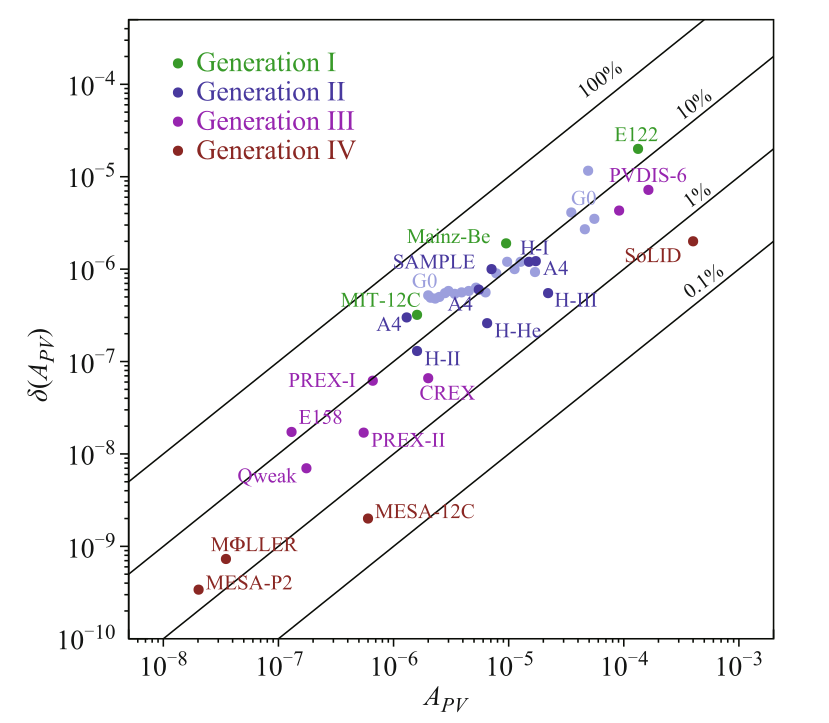
\includegraphics[width=0.5\linewidth]{PVES}
    \caption{Evolution of PVES experiments, solid lines represent the relative 
    precision. Generation I experiments (E122 (1978) \cite{PRESCOTT1978347}, 
    MIT-12C (1989) \cite{PhysRevLett.65.694} and Mainz-Be (1990) \cite{HEIL19891}) 
    did pioneering work to pave the way for PVES. Generation II experiments
    (the SAMPLE collaboration \cite{SAMPLE} at the MIT-Bates accelerator, 
    the G0 \cite{G0} and HAPPEX \cite{HAPPEX} collaboration at Jefferson Lab and
    the A4 collaboration \cite{A4} at the Maizer Mikrotron (MAMI) accelerator) 
    were devoted to the exploration of strange FFs in nucleons.
    Generation III experiments (E158 at SLAC \cite{PhysRevLett.95.081601}, 
    Qweak \cite{PhysRevLett.111.141803} and PVDIS \cite{PhysRevLett.111.082501})
    tested the SM at low energy and measured the neutron skin thickness of nuclei
    (PREX-I/II and CREX). The planned Generation IV experiments (SoLID program \cite{SoLID}
    and M\\OLLER experiment \cite{Moller} at JLab, P2 experiment on the future
    Mainz Energy-recovery Superconducting Accelerator (MESA) \cite{MESA-P2})
    will continue to test the SM and explore the structure of nucleons with higher precisions.
    (MESA-12C is the same experiment as MESA-P2 with a different \C target) }
\end{figure}

Generally, PVES experiments requries 2 experimental conditions: polarized electron
beam and fast flipping of beam polarization. Both requirements actually come to 
the same dependence: an intense source of polarized electrons and with quick response. 
The nature of being PV means measurement between different polarization states, 
while the \textbf{tiny} characteristic of PV asymmetry
demands fast flipping of the polarization states.
To measure such a tiny quantity, it is essential to control
the experimental configurations as the same as possible between different
beam helicities. One obvious and effective method to do the job is to fast 
flipping of beam helicity, the faster the helicity reversal, the smaller
the possible change in beam conditions, target density and other apparatus, the smaller
the introduced false asymmetry. This requirement makes PVES out of the capacity
of storage ring accelerators.
% The key for PVES experiments is the fast flipping ($10^2 - 10^3\ Hz$) of beam helicity to reduce 
% the random noise caused by fluctuations in target density and the beam qualities, that
% means it is out of the capicity of storage ring accelrators and 
% PVES depends on the development of the intense source of polarized electrons.
Though of the fast reversal of electron's helicity, much effort is needed to
control the beam fluctuation, making it as small as possible. Possible systematic
uncertainties in the source and accelerator will be controlled through the slow
reversal of beam helicity. In terms of the target deformity under electron bombarment,
a raster with very high scanning rate will minimize this uncertainty. As for 
detection of scattered electrons, electron flux rather than single electron will
be counted due to high scattering rate in such experiments.

The 2 sister experiments were conducted in Hall A at JLab, the CEBAF accelerator 
at JLab is one of the few facilities in the world that can do PVES experiments (
other facilities include MIMA and its successor MESA, the Facility for Antiproton
and Ion Research (FAIR) and the Facility for Rare Isotope Beams (FRIB)). CEBAF 
provided excellent polarized electron beams (helicity correlated difference at 
sub-nanometer level) to hall A, with dedicated apparatus 
(Compton polarimeter, taget chamber, HRS and others) in Hall A, we were able 
to measure this tiny asymmetry precisely.

% table of beam parameters
\begin{table}[h]
    \centering
    \begin{tabular}{l | c c }
	\hline
	&   PREX-II & CREX  \\
	\hline
	Target	& \Pb	& \Ca	\\
	Target density ($g/cm^3$)   & 11.38 & 1.855	\\
	Target thickness ($mm$)	& 0.2554 + 0.5520 + 0.2566	& 6	\\
	Number of Target & 10 & 1 + 1	\\
	Used	& 6 & 2	\\
	\hline
	Beam Energy ($GeV$) & 0.953 & 2.18  \\
	Largest Beam Current ($\mu A$)	& 70	& 150	\\
	Average Beam Polarization ($\%$) & 89.7   & 87.1   \\
	Beam Rate ($MHz$) & 249.5	& 249.5 \\
	Electrons/Bunch	($\times 10^6$)	& 1.75	& 3.76	\\
	Helicity Flip Rate ($Hz$)  & 240   & 120   \\
	Power on Target ($Watt$)	&   &	\\
	\hline
	Scattering angle ($\deg$)   & 4.7	& 4.51 \\
	$Q^2$ ($GeV^2$)	& 0.00616   & 0.0297	\\
	Scattering rate ($MHz/arm$)   & 576\footnote{This rate doesn't include the contribution from the diamond foils}   & 13 \\
	xsection ($mbarn$)    & 3930.6	& 5.3   \\
	Acceptance ($msr$)    &	0.0037 & 0.0037  \\
	\hline
	Collected Charge ($C$)	& 114	& 412	\\
	\hline
	Predicted $\CA_{pv}$ ($ppm$)	& 0.6   & 2 \\
	Proposed precision  & 3.6\%   & 2.4\% \\
	Error on $R_n$ ($fm$)	& 0.06	& 0.02	\\
	\hline
    \end{tabular}
    \caption{Summary of PREX-II and CREX}
    \label{tb:parameters}
\end{table}

%%%%%%%%%%%%%%%%%%%%%%%%%%%%%%%%%%%%%%%%%%%%%%%%%%%%%%%%%%%%%%%%%%%%%%%%
\section{Kinematics}
PREX-II and CREX are follow-up experiments to PREX-I, which also ran at JLab in 2010. 
With excellent control of systematic uncertainty, but unfortunately, 
many technical challenges during the experiment, PREX-I's result was statistics 
limited, achieving a precision of 10\% \cite{PhysRevLett.108.112502}:
$$ \CA_{Pb} = 656 \pm 60 (stat) \pm 14 (syst) \ ppb$$
Based on the experience and lessons we learned from PREX-I, 
PREX-II and CREX had more well-established designs, which helped to
meet the goal of high-precision.

One important feature of these 2 experiments is the redundancy design for critical
components: we have 2 slow helicity reversal for systematic uncertainty control,
we have 2 polarimeters for polarization measurement, we have multiple BPMs and
BCMs for beam parameter monitoring, we have multiple Pb foil targets and finally
2 HRS arms for electron reception.

%%%%%%%%%%%%%%%%%%%%%%%%
\subsubsection{Uncertainty Budget}
The goal of PREX-II is to achieve the 1\% precision in \Pb neutron radius proposed
by PREX-I, which requires the presicion of PV asymmetry measurement better than 3\% \cite{PhysRevLett.106.252501}. 
CREX proposed similar goal, that a precision of $0.02 \ fm$ (0.6\%) in the
\Ca neutron radius will be an essential benchmark to test various microscopic 
models, which correspond to a 2.4\% total error in PV asymmetry.

% page 7 in https://prex.jlab.org/DocDB/0000/000065/001/kutz_fom.pdf
As said above, PREX-I already had impressive control over systematic uncertainties (2.1\%),
so will the PREX-II and CREX. The main concern is to collect as much scattered 
electrons as possible to reduce statistical error, which is inversely 
proportional to $\sqrt{N}$.
\begin{table}
    \centering
    % page 19 in https://www.jlab.org/intralab/calendar/phys_seminar/2019/JLabtalk_20190206mod_Palatchi.pdf
    \begin{tabular}{c| c c}
	\hline
	Experiment  & PREX-II (\%)	& CREX (\%)	\\
	\hline
	Charge Normalization	& 0.1	& 0.1	\\
	Beam Asymmetry		& 1.1	& 0.3	\\
	Detector Non-Linearity	& 1.0	& 0.3	\\
	Transverse Asymmetry	& 0.2	& 0.1	\\
	Polarization		& 1.1	& 0.8	\\
	Target Contamination	& 0.4	& 0.2	\\
	Inelastic Scattering	& $<0.1$    & 0.2   \\
	Effective $Q^2$		& 0.4	& 0.8	\\
	\hline
	Total Systematic	& 2	& 1.2	\\
	Statistical		& 3	& 2.4	\\
	\hline
	Total			& 3.6	& 2.7	\\
	\hline
    \end{tabular}
    \caption{Budget of systematic and statiscal error in both experiments 
    \cite{prex-II_proposal, crex_proposal}
    }
\end{table}

\begin{equation}
    \frac{\delta \CA}{\CA} = \sqrt{\sigma^2_{stat} + \sigma^2_{sys}}	\qquad 
    \sigma_{stat} = \frac{\sigma_{det}}{P\sqrt{N}}
\end{equation}
where:
\begin{itemize}
    \item $\sigma_{det}$ is the detector uncertainty
    \item P is the beam polarizaiton
    \item N is the total number of scattered electrons
\end{itemize}

%%%%%%%%%%%%%%%%%%%%%%%%
\subsection{Figure Of Merits (FOM)}
The choice of beam energy and scattering angle is a compromise of competing
factors. PV asymmetry prefers larger beam energy and larger scattering angle,
while scattering rate falls dramatically with beam energy and scattering angle,
$Q^2$ also likes smaller beam energy and scattering angle, and calculation 
showes that the sensitivity of PV asymmetry w.r.t. neutron radius is oscillating
along beam energy. All these considerations are incorporated into the FOM, which
is defined as:
\begin{equation*}
    \text{FOM} = R \times \CA^2 \times \epsilon^2
\end{equation*}
where R is the scattering rate, $\CA$ the PV asymmetry and $\epsilon$ 
the sensitivity of $\CA$ w.r.t. $R_n$. One difference here is that FOMs for most PVES 
experiments have only R and $\CA^2$, the inclusion of $\epsilon$ in our FOM help
to achieve a higher precision in $R_n$ measurement.

%%%%%%%%%%%%%%%%%%%%%%%%
% from materials/rate_estimation.pdf
\subsubsection{Rate}
For a data set of N independent events sampled from one normal distribution 
$X\sim N(x_0, \sigma_0)$, the statistical uncertainty on the measured mean value
will be:
$$ var(\bar{x} = \frac{1}{n}\sum x_i) = \frac{1}{n^2}var(x_i) = \frac{\sigma_0^2}{n} 
\quad \Longrightarrow \sigma(\bar{x}) = \frac{\sigma_0}{\sqrt{n}} $$

Assume one want to measure a $1 \ ppm$ asymmetry to 1\% statistical uncertainty,
\begin{equation}
    \frac{\sigma_A}{A} = \frac{1}{A}\frac{\sigma_{det}}{\sqrt{2N}} 
    \approx \frac{1}{A\sqrt{2N}} = 1\% \quad 
    \Longrightarrow N = 5 \times 10^{15} 
    \label{eqn:statistical_error}
\end{equation}
a factor of 2 is included because we have 2 HRS arms.
One need to count $\sim10^{15}$ scattered electrons. Given a counting rate of $1\ MHz$, 
it will take $\frac{5\times 10^{15}}{1\ MHz} = 5\times 10^{9}\ s \approx 160 \ years$,
a completely unacceptable time scale. So we have to turn to integrated flux technique
for a higher scattering rate, which is:
\begin{equation}
    \frac{dR(\theta)}{d\Omega} = \frac{d\sigma}{d\Omega}\ I\ t\ \frac{\rho}{A} \times N_A   
\end{equation}
\begin{itemize}
    \item $\frac{d\sigma}{d\Omega}$ is the fractional cross section in $cm^2/str$,
    \item I is the beam current in $electrons/s$
    \item t is the target thickness in $cm$
    \item $\rho$ is the target density in $g/cm^{3}$
    \item A is the atomic number
    \item $N_A = 6.022\times 10^{23}$ is the Avogadro's constant and conversion factors.
\end{itemize}

The differential cross section was numerically calculated by our theoretical friends
with values of $3930.6 \ mbarn$ and $5.3 \ mbarn$ for \Pb and \Ca at their corresponding
kinematics. Other parameters can be checked in table \ref{tb:parameters}.

The total rate will be the integration over the acceptance:
\begin{equation}
    R = \int \frac{dR(\theta)}{d\Omega} d\Omega = \frac{dR}{d\Omega} d\Omega
\end{equation}
PREX-II and CREX have an acceptance defined by the septum and Q1 collimator, which
is $d\Omega = 0.0037 \ str$

Finally, we should also consider radiative correction due to emission of virtual
and real soft photons (Bremsstrahlung), and hard photons by vacuum polarization,
this correction is formulated as:
\begin{equation}
    \eta = \left(\frac{\Delta}{E} \right)^{bt}
\end{equation}
which is evaluated to be: $\eta \sim 0.5$.

\begin{figure}[h!]
    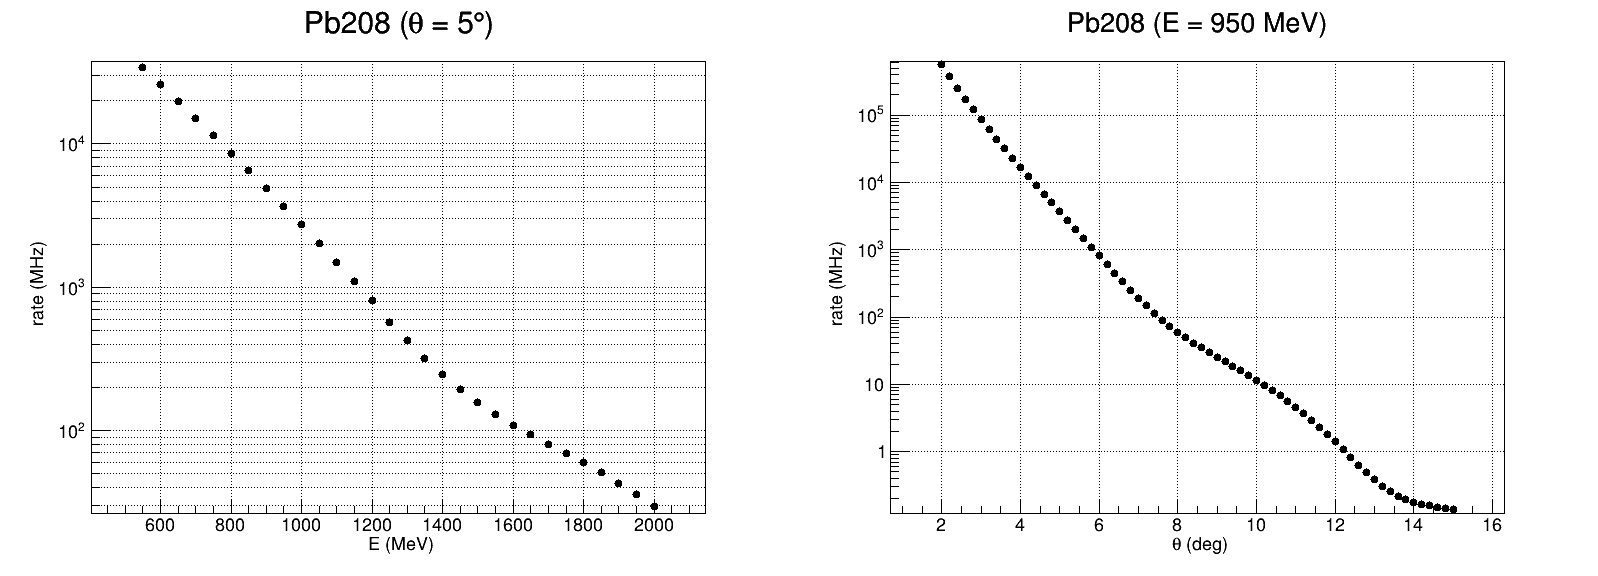
\includegraphics[width=0.5\linewidth]{Pb208_rate}
    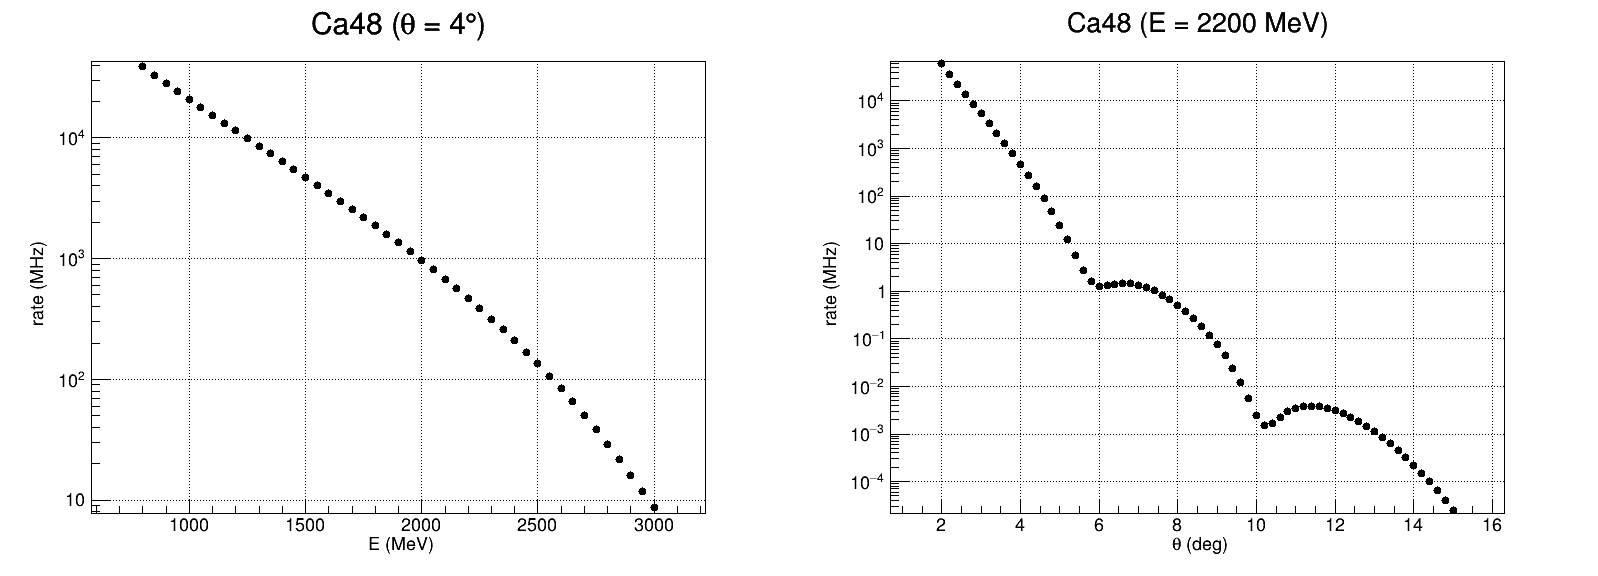
\includegraphics[width=0.5\linewidth]{Ca48_rate}
    \caption{Scattering rate versus beam energy and scattering angle for \Pb and \Ca,
    the energy and scattering angle are design values.
    We see that rate falls quickly along both beam energy and scattering angle for
    both nuclei, so one would like small beam energy and small scattering angle (equivalently
    small $\vec{q}$) for large scattering rate.}
\end{figure}

%%%%%%%%%%%%%%%%%%%%%%%%
\subsubsection{Asymmetry and Sensitivity}
As we shown in eq. \ref{eqn:statistical_error}, the asymmetry itself matters,
a 2 times larger asymmetry means we can reduce the run time to one quarter,
a huge save of beam time. So we should choose the kinematics region where
asymmetry is large. Besides, asymmetry's sensitivity ($\epsilon$) to neutron radius is
also important, keep in mind that our final goal is to extract neutron radius
from PV asymmetry, the more sensitive the asymmetry to neutron radius, the
more precise the extracted neutron radius. The sensitivity is calculated
as the relative change of $\CA$ with 1\% change in neutron radius.
\begin{equation}
    \epsilon = \frac{\delta \CA/\CA}{\delta R/R} = \frac{|\CA_{stretched} - \CA|/\CA}{1\%}
\end{equation}
Though asymmetry is what we want to measure, we can estimate its value based
on some theoretical models, as was numerically calculated by our theoretical 
friends in \cite{PhysRevC.57.3430}.
\begin{figure}[h!]
    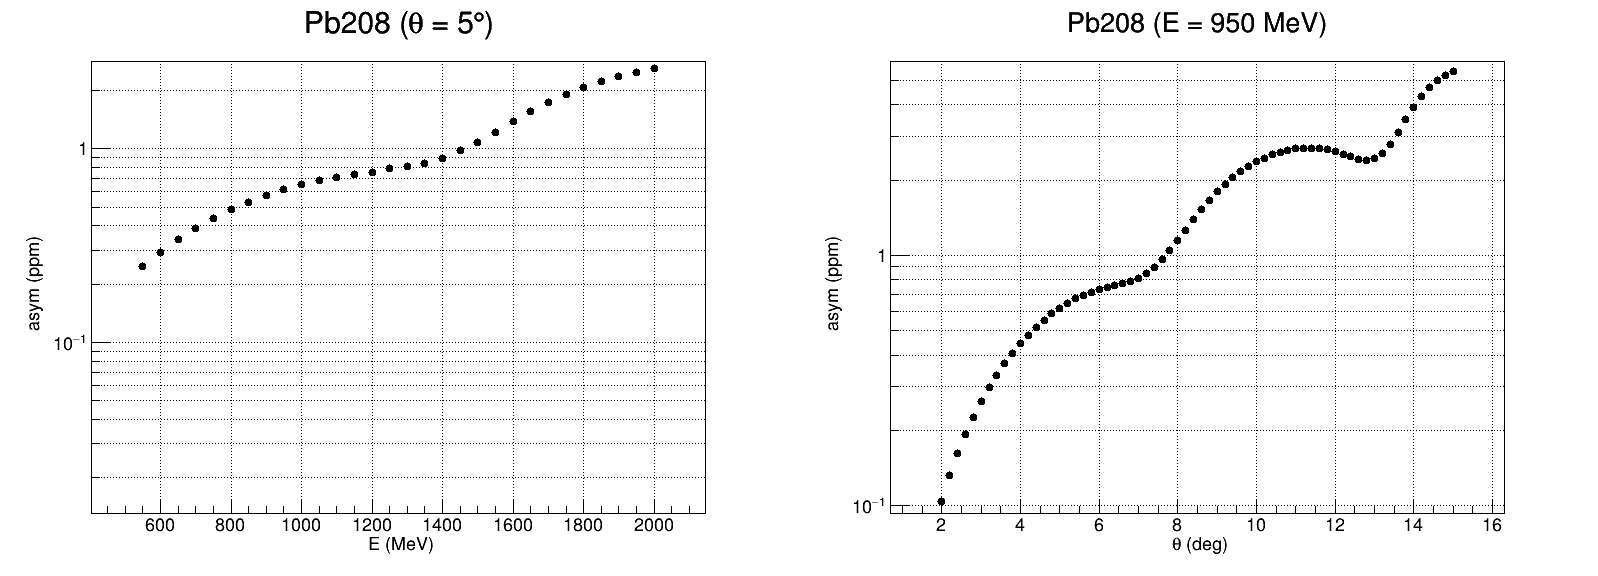
\includegraphics[width=0.5\linewidth]{Pb208_asym}
    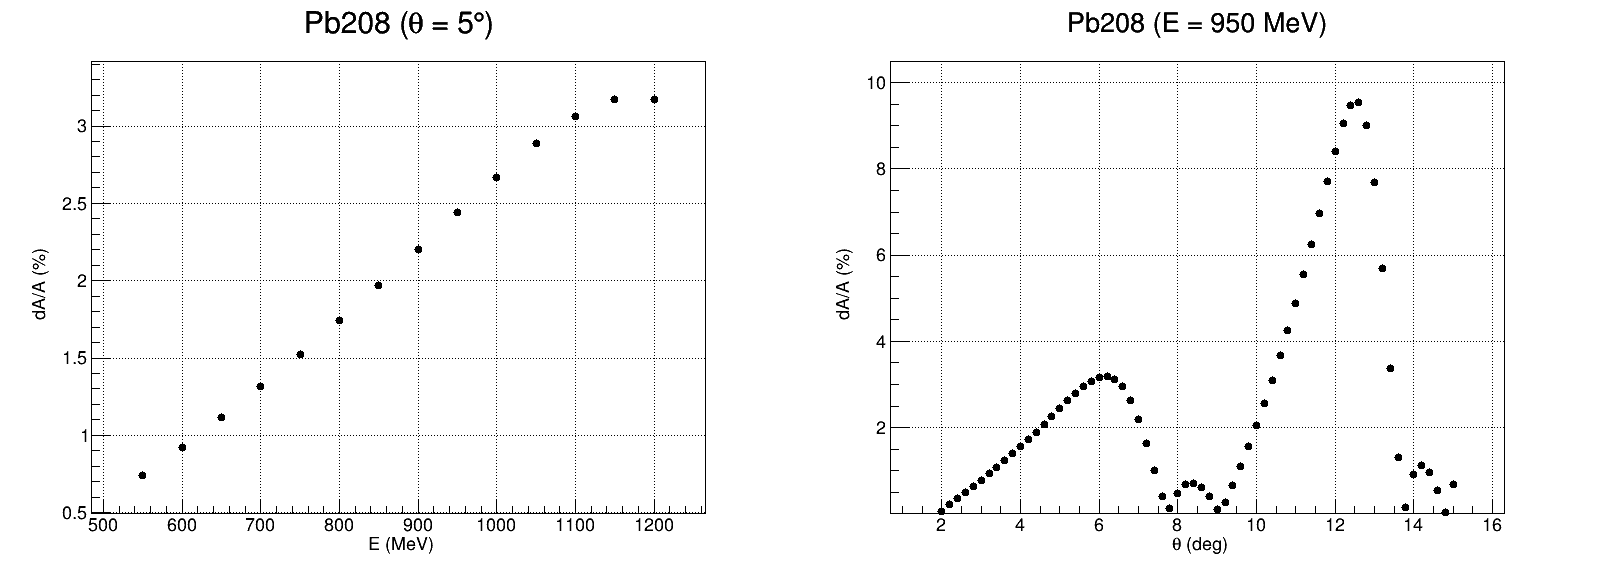
\includegraphics[width=0.5\linewidth]{Pb208_sen}
    \caption{Asymmetry and sensitivity plot for \Pb, which increases along beam 
    energy and oscillating up along scattering angle. The sensitivity plot is
    calculated with 1\% change in neutron radius and it shows the absolute value.
    So in small scattering angle region, there is a local maximum around $6^\circ$}
\end{figure}
\begin{figure}[h!]
    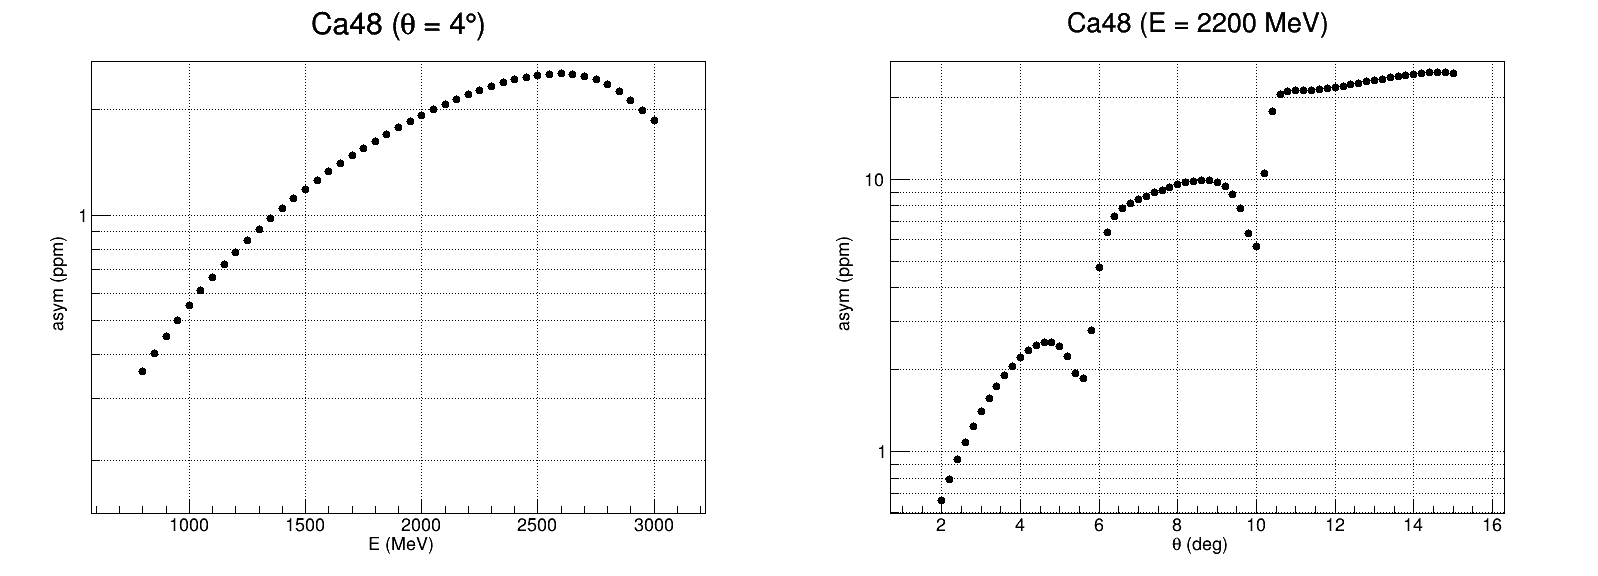
\includegraphics[width=0.5\linewidth]{Ca48_asym}
    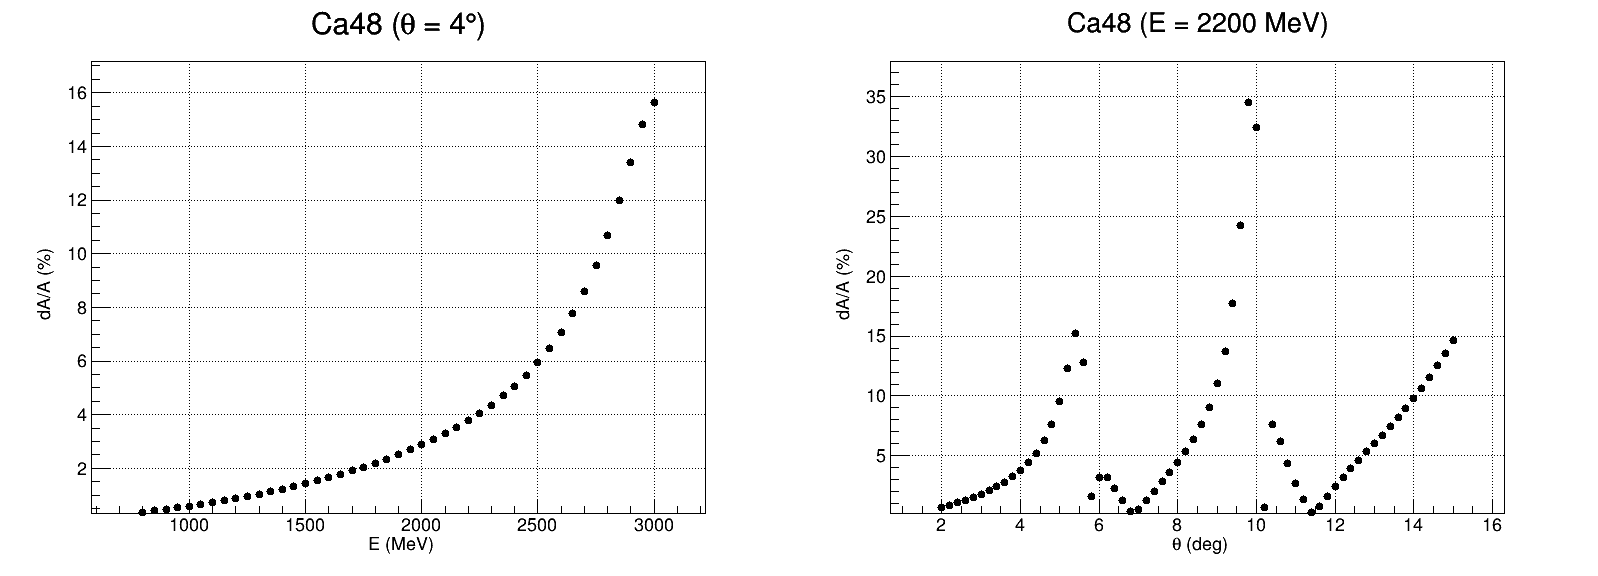
\includegraphics[width=0.5\linewidth]{Ca48_sen}
    \caption{Asymmetry and sensitivity plot for \Ca, the asymmetry maximize around
    2500 MeV and there is a local maximum about $4.5^\circ$. As for sensitivity,
    there is regional maximum around $5^\circ$}
\end{figure}

Based on the theoretical result, we can optimize the kinematics for both nuclei:
\begin{equation}
    \frac{\delta R}{R} = \frac{\delta \CA}{\CA} \frac{1}{\epsilon} 
	= \frac{\sigma_{det}}{P} \frac{1}{\sqrt{N} \CA \epsilon}
\end{equation}
To minimize $\delta R/R$, it is equivalent to maxize 
\begin{equation}
    FOM = N\times \CA^2 \times \epsilon^2
\end{equation}
\begin{figure}
    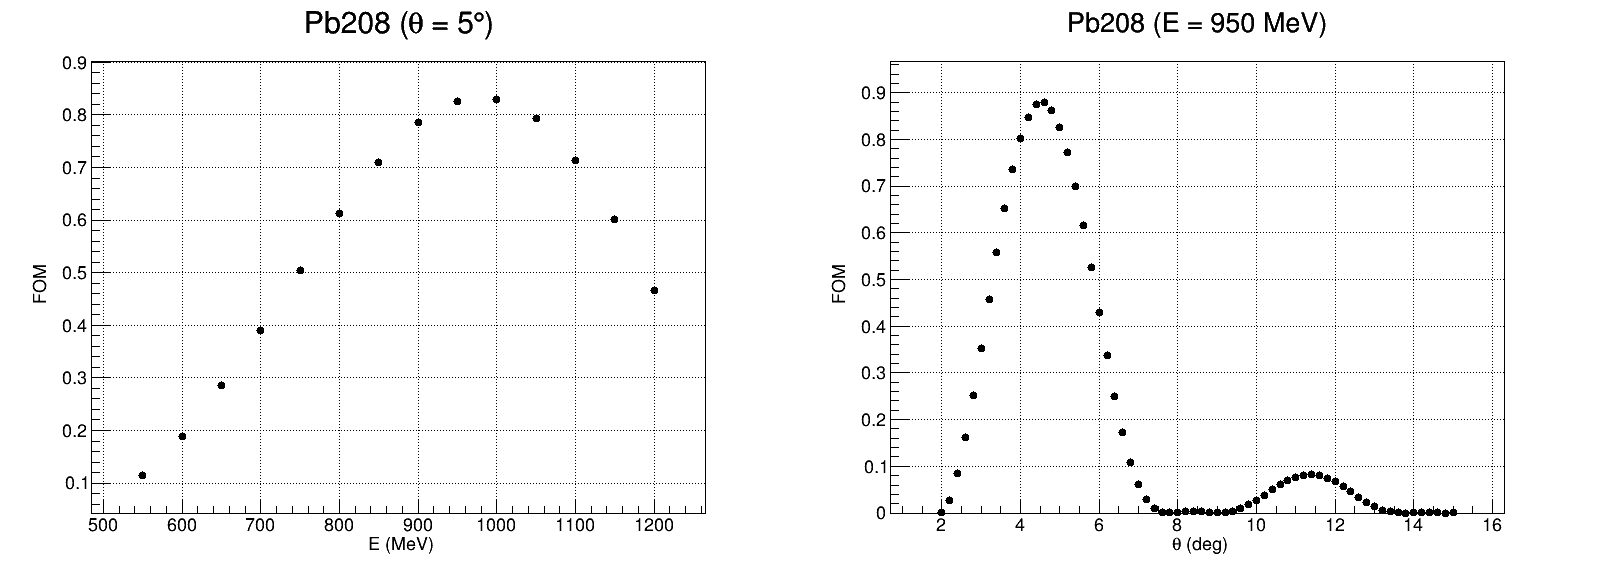
\includegraphics[width=0.5\linewidth]{Pb208_fom}
    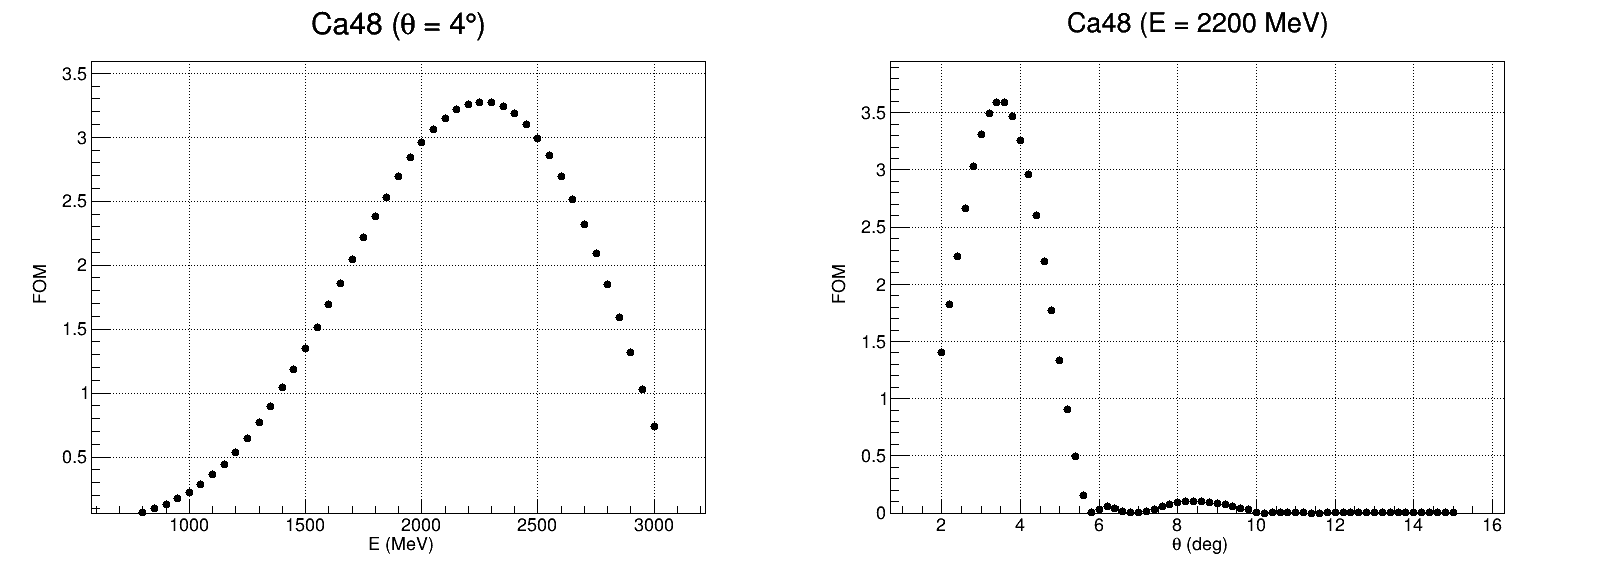
\includegraphics[width=0.5\linewidth]{Ca48_fom}
    \caption{For both nuclei, FOM supports a small scattering angle. As for beam energy,
    FOM maximize around 950 (2200) $GeV$ for \Pb (\Ca).}
\end{figure}

The design values of beam energy and scattering angle were chosed to be 950 (2200) $MeV$
and 5 (4) $degree$ for \Pb (\Ca). The beam energy of CREX is exactly 1-pass beam
energy in CEBAF.
\begin{comment}
    The measured asymmetry will be:
    \begin{equation*}
	\CA = \frac{2\pi}{R} \int \CA_0(\theta)R(\theta)d\theta
    \end{equation*}

    For PREX-II: average sensitivity reduced by 5\% due to ${}^{12}C$ contamination
    For CREX: average sensitivity reduced by 10\% due to ${}^{40}Ca$ contamination

%%%%%%%%%%%%%%%%%%%%%%%%
% \subsubsection{Factor of 1.06}
    While a quartz Cerenkov detector is valued for radiation hardness and insensitivity to soft backgrounds, there is a particular challenge for few GeV electrons. In this energy range, shower fluctuations in a thick or radiated detector significantly degrade energy resolution, while photon statistics degrade the energy resolution for a thin detector. The energy resolution $\Delta E$ at nominal electron energy E increases the statistical error that one would have with infinite resolution $\sigma_0$ to obtain the total statistical error:
$$ \sigma = \sigma_0\sqrt{1+\left(\frac{\Delta E}{E}\right)^2}$$
    
Based on experience in the PREX experiment, we expect an reduction of statistical precision of a factor of 1.06 due to detector resolution.

\bigskip
Using HRS of Hall A, a \textbf{small} scattering angle maximizes the FOM. 
Given practical constraints on how low an angle ($4^\circ$) we can reach with 
septum magnets, the energy is fixed and turns out to be 2.2 GeV, which is a 
natural 1-pass beam energy for CEBAF operations in the 12 GeV era.
\end{comment}

%%%%%%%%%%%%%%%%%%%%%%%%%%%%%%%%%%%%%%%%%%%%%%%%%%%%%%%%%%%%%%%%%%%%%%%%
\section{Continuous Electron Beam Accelerator Facility (CEBAF)}
\begin{figure}[h!]
    \begin{subfigure}[b]{0.59\textwidth}
    \begin{tikzpicture}
	\begin{scope}
	    \node[anchor=south west, inner sep=0] (image) at (0, 0)
	    { 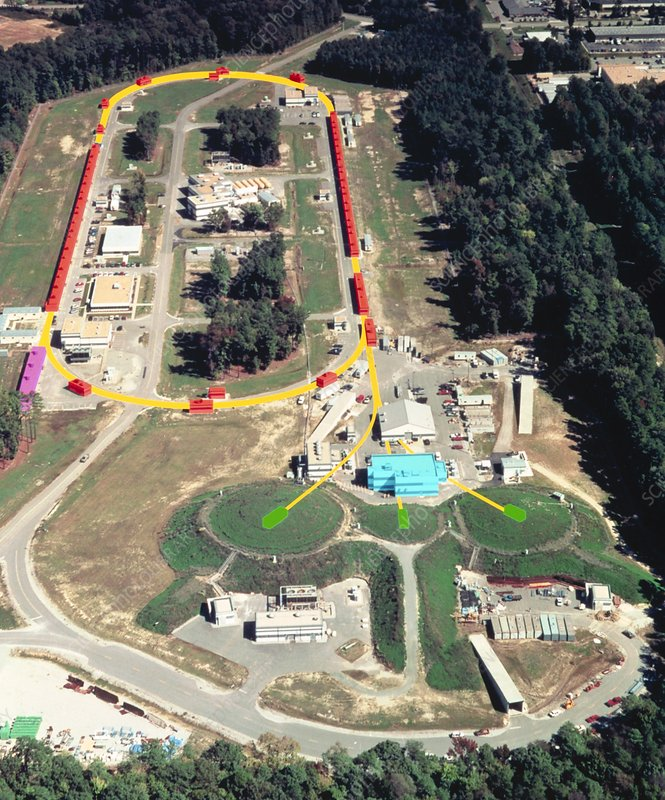
\includegraphics[width=\linewidth]{jlab.jpg} };
	    \begin{scope}[x={(image.south east)}, y={(image.north west)}]
		\node [red] at (0.415, 0.355) {\textbf{A}};
		\node [red] at (0.610, 0.355) {\textbf{B}};
		\node [red] at (0.780, 0.355) {\textbf{C}};
	    \end{scope}
	\end{scope}
    \end{tikzpicture}
    \end{subfigure}
    \begin{subfigure}[b]{0.5\textwidth}
	\includegraphics[width=0.9\linewidth]{tunnel_construction}
	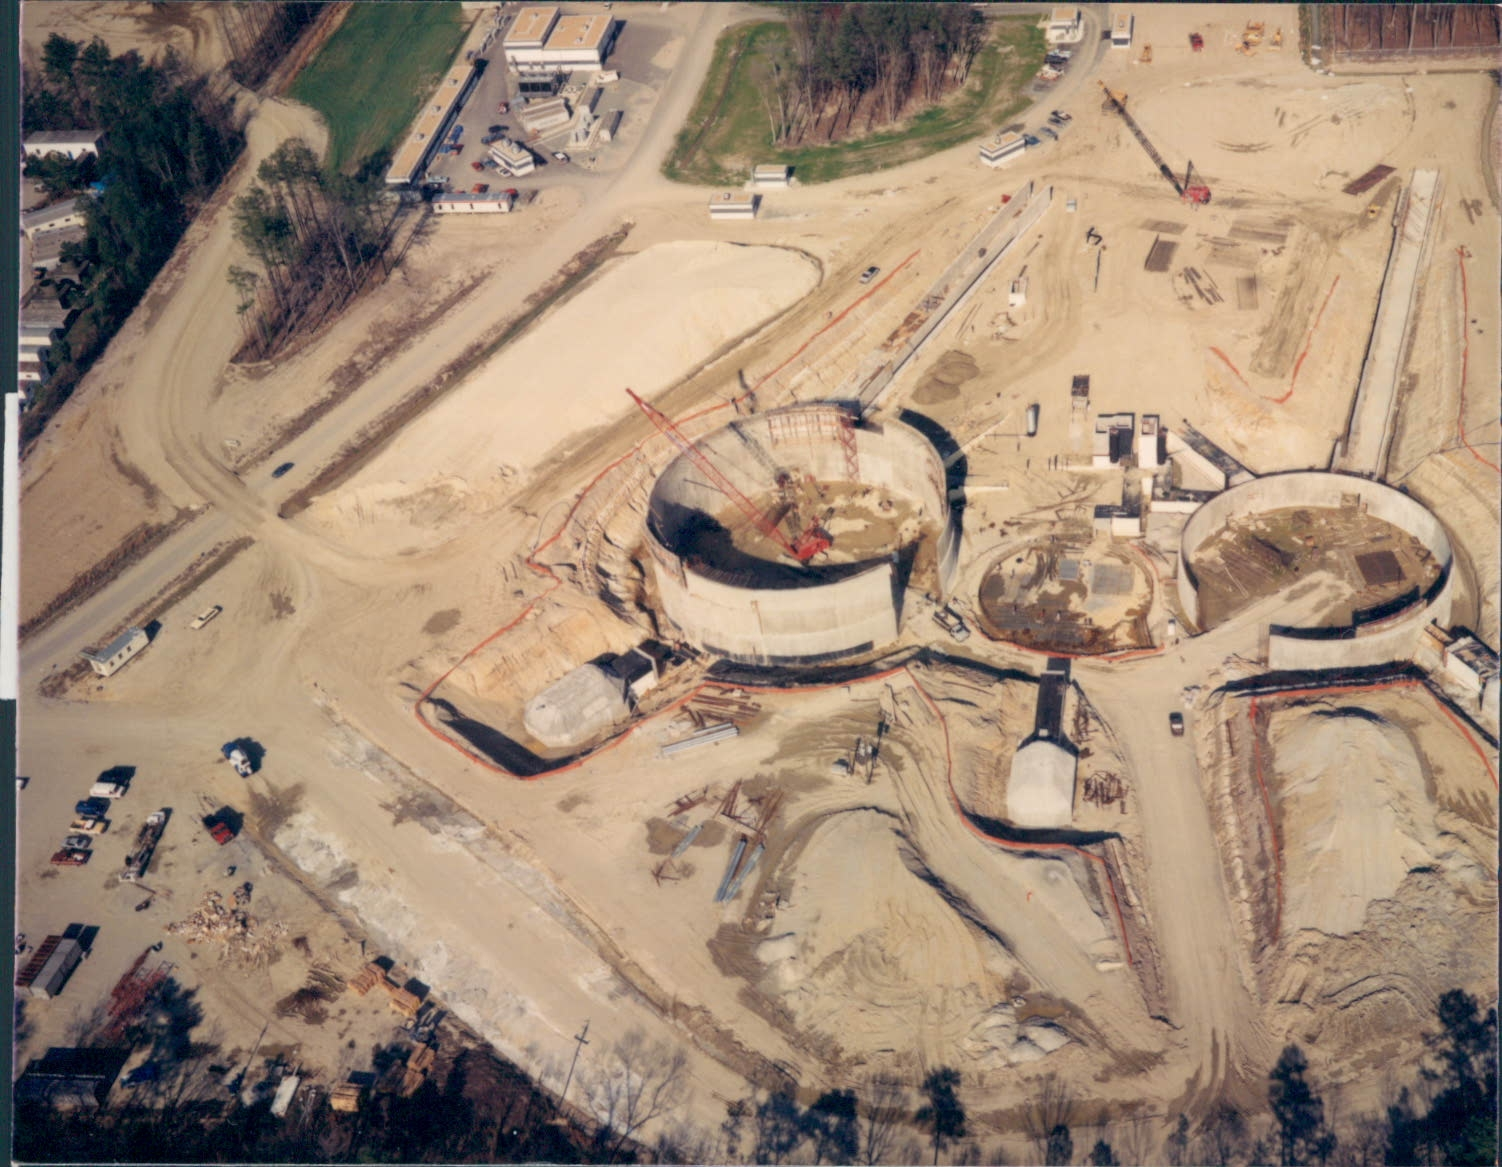
\includegraphics[width=0.9\linewidth]{hall_construction}
    \end{subfigure}

    \caption{Aerial view of JLab accelerator site, yellow line tells the position
    of the CEBAF accelerator and the 3 experimental halls are marked out as A/B/C 
    (Hall D locates on the top left corner, after the exit of north LINAC).
    The accelerator tunnel is $30 \ feet$ ($\sim 9 \ m$) underground and $10 \ feet$ ($\sim 3 \ m$) 
    high, with a circumference of about $7/8\ miles$ ($1.4\ km$). There are 2 superconducting 
    LINAC (red lines), each of $1/4\ miles$ ($400\ m$). The pink part on the mid
    left is the location of injector. The right 2 plots show the tunnel and 
    experimental halls under construction.}
\end{figure}

\begin{figure}[h!]
    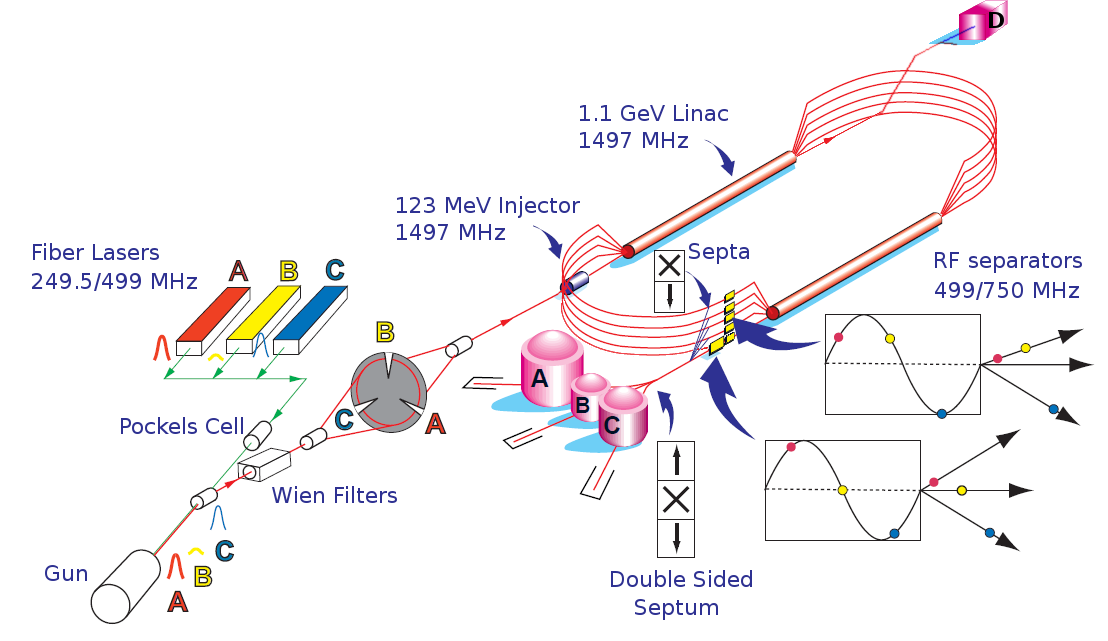
\includegraphics[width=0.9\linewidth]{cebaf.png}
    \caption{Schematic plot of CEBAF. Low energy beams will be kicked into 
    higher arc, and high energy beams will go through lower arc. The magnetic
    field increases from higher arc to lower arc to keep electron trajectory 
    have the same radius.}
    \label{fig:cebaf}
\end{figure}
CEBAF is able to deliver multi-GeV continuous wave (cw) eletron beams of different
energies and different intensities to 4 halls simultaneously.
With the 12 GeV upgrade, the north and south $1497\ MHz$ LINAC each has 25 
Superconducting Radial Frequency (SRF) cryomodules, capable of accelrating 
electrons at the peak rate of 2.2 $GeV/turn$. Hall A, B and C can receive up
to $2.2 \times 5 = 11 \ GeV$ cw beams and Hall D, with an extra half circle,
can receive up to $12\ GeV$ cw beams. With this design, different nuclear 
experiments can be carried out in different halls without interfering each other,
theoretically.

As one can see in \ref{fig:cebaf}, laser pulse ($\lambda = 780 \ nm$) from 4 lasers 
(Hall D laser is not shown in the plot) shoot in the electron gun 
(2 electron guns in total) that 
operates at $-130\ kV$ to excite electrons, which interweaving with each other, 
forming a chain of electron bunches, with a phase difference of $120^\circ$ from 
neaby bunches (Hall D doesn't have its own slit in the chopper, therefore 
it follows either Hall A or Hall C). This electron chain is sent into north LINAC
by the injector, accelerated by both LINACs. After reaching desired energy,
they will be kicked out at the exit of south LINAC and delivered to experimental
halls (A, B and C) for various experiments. 

The maxium beam current of $200\ \mu A$ at (old) highest energy of $5\ GeV$ 
available at CEBAF is limited by the rf power ($1\ MW = 5\ GeV \times 200\ \mu A$) 
and by the beam power on the beam dump. While Hall B and D requires only tiny 
amount of cw beams (at $nA$ level), it is actually Hall A and C that consume 
the produced electron beams, both can receive a few tenths to over one 
hundred $\mu A$.

While all 4 halls at JLab are dedicated to the study of nuclear structure, they
focus on different aspects. Hall A concentrates on form factors of various nuclei, 
Hall B digs into generalized parton distributions, Hall C devotes itself to precise
determination of valance quark properties in nuclei, and finally, the newly 
established Hall D explores origin of confinement through exotic mesons.

Because all 4 halls shared the same electron source and the same accelerator, 
cooperation is needed to make them work at the same time. In terms of electron
source, PVES experiment usually has priority over other experiments to maintain 
the quality of polarized electron beam. As for the LINAC, if one hall wants
a smaller energy, say $1\ GeV$, then the LINAC power will be reduced to $1\ GeV/turn$,
which will be applied to other halls' electron beams, therefore limiting the 
highest energy available in other halls. Careful schedule is needed to make sure
every hall get what they want.
%%%%%%%%%%%%%%%%%%%%%%%%%%%%%%%%%%%%%%%%%%%%%%%%%%%%%%%%%%%%%%%%%%%%%%%%
\section{Polarized Electron}
% The key to the success of this experiment was the 1975 discovery of a new method for producing
% polarized electrons made by a group in Colorado, which included E.L. Garwin of SLAC.
% Shortly thereafter, a new source was built for the SLAC linac utilizing the method, thus
% allowing for the 1978 parity violation measurements which were in close agreement with
% those predicted by the GWS model. 

%%%%%%%%%%%%%%%%%%%%%%%%%%%%%%%%%%%%%%%%%%%%%%%%
\subsection{Polarized Electron Source}
PVES experiments motivate the development of polarized electron source, which 
require a highly stable polarized electron source that can produce
high polarization electron beam at a wide range of intensity, from nA to A 
depending on the experiment. The source should be capable of rapid helicity
reversal ($\sim 100 Hz$) with negligible impact on other properties of the beam.

Currently, GaAs-based semiconductor photoemission source is % confirmed by Wang Yan
the only available polarized electron source for accelerators on the market.
Historically, this 
kind of electron source was the only one that could satisfy high peak currents 
required by the low duty factors of the old accelerators and rapid helicity 
reversal required by PVES. That's why it is the only player on the market now.
Over the past few decades, pulsed beam has been replaced by continuous beam while
this electron source is inheritated and further developed. The polarized electron
source used by CEBAF can produce electron beam with polarization greater than
85\%, much larger than the 37\% polarization from its inauguration at SLAC. \cite{PRESCOTT1978347}

The design was first proposed independently by Garwin, Pierce and Siegmann \cite{GARWIN}
and by Lampel and Weisbuch \cite{LAMPEL1975877}. The idea is straightforward:
When circularly polarized laser light with carefully selected energy $E_{gap} < h\nu < E_{gap} + \Delta$
shoot on the semiconductor, only electrons on the valance band $P_{3/2}$ will be
pumped into the conduction band $S_{1/2}$. The selection rule makes sure only
those transitions that satisfy $\Delta m_j = +1 \ (-1)$ can occur for circularly
right (left) incoming photons, As shown in fig. \ref{fig:excitation-b}.
The ratio of the transition rate is also marked out in circle in the plot, 
which can be calculated from the Clebsch-Gordan coefficient easily. The excited
electrons are polarzied and different states have different pumping rate, so
we have polarized electron beam now with polarization as: P = (3-1)/(3+1) = 50\%,
for both cases.
\begin{figure}[h!]
    \tikzmath{\yone=1.3; \ytwo=2.5; \ythree=5;} 
    \centering
    \begin{subfigure}[b]{0.49\textwidth}
	\centering
	\begin{tikzpicture}
	    \centering
	    \begin{axis}[axis lines=middle,
		xmin=-1.4, xmax=2.75,
		ymin=0, ymax=7,
		xlabel={\large $k$},
		ylabel={\large$E$},
		xlabel style={below},
		xtick=\empty,
		ytick=\empty,
		x axis line style={draw=none},
		% clip=false,
		]
		\addplot[Violet, line width=3pt, samples=100, domain=-0.7:0.7, name path=A] {-2*x^2 + \yone};
		\addplot[OliveGreen, line width=3pt, samples=100, domain=-0.7:0.7, name path=B] {-2*x^2 + \ytwo};
		\addplot[OliveGreen, line width=3pt, samples=100, domain=-0.7:0.7, name path=B] {-1.2*x^2 + \ytwo};
		\addplot[Blue, line width=3pt, samples=100, domain=-0.7:0.7, name path=B] {2*x^2 + \ythree};
		\draw [/pgfplots/every inner x axis line, draw=black] (0,0) -- (\pgfkeysvalueof{/pgfplots/xmax}, 0); 
		\draw [dashed, draw=black] (0,\yone) -- (\pgfkeysvalueof{/pgfplots/xmax}, \yone);
		\draw [dashed, draw=black] (0,\ytwo) -- (\pgfkeysvalueof{/pgfplots/xmax}, \ytwo);
		\draw [dashed, draw=black] (0,\ythree) -- (\pgfkeysvalueof{/pgfplots/xmax}, \ythree);
		\draw [stealth-stealth, thick] (0.8, \yone) -- (0.8, \ytwo) node [midway, right] {\bm{$\Delta = 0.34\ eV$}};
		\draw [stealth-stealth, thick] (0.8, \ytwo) -- (0.8, \ythree) node [midway, right] {\bm{$E_{gap} = 1.42\ eV$}};
		\node [Violet, below] at (-1, \yone) {\large\bm{$P_{1/2}$}};
		\node [OliveGreen, below] at (-1, \ytwo) {\large\bm{$P_{3/2}$}};
		\node [Blue, above] at (-1, \ythree) {\large\bm{$S_{1/2}$}};
		\node [left, above] at (-0.2, \ytwo) {\large\bm{$E_F$}};
	    \end{axis}
	    \label{fig:excitation-a}
	\end{tikzpicture}
    \end{subfigure}
    \hfill
    \begin{subfigure}[b]{0.49\textwidth}
	\centering
	\begin{tikzpicture}
	    \begin{axis}[axis lines=middle,
		xmin=0, xmax=8,
		ymin=0, ymax=7,
		xlabel={\large $m_j$},
		ylabel={\large$E$},
		xlabel style={below},
		xtick=\empty,
		ytick=\empty,
		]
		\draw [/pgfplots/every inner y axis line, draw=black] (6.5,0) -- (6.5, \pgfkeysvalueof{/pgfplots/ymax}) node [below right] {\large J}; 
		\draw [draw=Violet, line width=2pt] (1.25,\yone) -- (2.25, \yone) node [midway, below, Violet] {\textbf{-1/2}};
		\draw [draw=Violet, line width=2pt] (4.25,\yone) -- (5.25, \yone) node [midway, below, Violet] {\textbf{+1/2}};
		\draw [draw=OliveGreen, line width=2pt] (0.5,\ytwo) -- (1.5, \ytwo) node [midway, below, OliveGreen] {\textbf{-3/2}};
		\draw [draw=OliveGreen, line width=2pt] (2,\ytwo) -- (3, \ytwo) node [midway, below, OliveGreen] {\textbf{-1/2}};
		\draw [draw=OliveGreen, line width=2pt] (3.5,\ytwo) -- (4.5, \ytwo) node [midway, below, OliveGreen] {\textbf{+1/2}};
		\draw [draw=OliveGreen, line width=2pt] (5,\ytwo) -- (6, \ytwo) node [midway, below, OliveGreen] {\textbf{+3/2}};
		\draw [draw=Blue, line width=2pt] (2,\ythree) -- (3, \ythree) node [midway, above, Blue] {\textbf{-1/2}};
		\draw [draw=Blue, line width=2pt] (3.5,\ythree) -- (4.5, \ythree) node [midway, above, Blue] {\textbf{+1/2}};
		\node [Violet, right] at (6.7, \yone-0.1) {\large\bm{$P_{1/2}$}};
		\node [OliveGreen, right] at (6.7, \ytwo-0.1) {\large\bm{$P_{3/2}$}};
		\node [Blue, right] at (6.7, \ythree-0.1) {\large\bm{$S_{1/2}$}};

		\draw [-stealth, Red, line width=2pt] (1, \ytwo) -- (2.5, \ythree) node [midway, circle, fill=CornflowerBlue, text=Black] {\textbf{3}};
		\draw [-stealth, Red, line width=2pt] (2.5, \ytwo) -- (4, \ythree);
		\node [above, Red] at (1, \ytwo+0.5) {\bm{$\sigma^+$}};
		\draw [-stealth, YellowOrange, line width=2pt] (4, \ytwo) -- (2.5, \ythree) node [midway, circle, fill=CornflowerBlue, text=Black] {\textbf{1}};
		\draw [-stealth, YellowOrange, line width=2pt] (5.5, \ytwo) -- (4, \ythree) node [midway, circle, fill=CornflowerBlue, text=Black] {\textbf{3}};
		\node [above, YellowOrange] at (5.5, \ytwo+0.5) {\bm{$\sigma^-$}};
	    \end{axis}
	\end{tikzpicture}
	\label{fig:excitation-b}
    \end{subfigure}
    \caption{Excitation of polarized electrons}
\end{figure}

\begin{figure}[h!]
    \centering
    \begin{subfigure}[b]{0.32\textwidth}
	\tikzmath{\yone=2.5; \ytwo=5; \ythree=9.5;} 
	\centering
	\resizebox{\textwidth}{0.33\textheight}{
	\begin{tikzpicture}
	    \centering
	    \begin{axis}[
		axis lines=middle,
		xmin=-3, xmax=1,
		ymin=0, ymax=10,
		hide axis,
		]
		\draw [dashed] (\pgfkeysvalueof{/pgfplots/xmin}, \yone) -- (0, \yone) node [right] {\bm{$E_F$}};
		\draw [dashed] (\pgfkeysvalueof{/pgfplots/xmin}, \ytwo) -- (0, \ytwo);
		\draw [dashed] (\pgfkeysvalueof{/pgfplots/xmin}, \ythree) -- (0, \ythree);
		\draw [Violet, line width=2pt] (0, 0) -- (0, \ythree) -- (\pgfkeysvalueof{/pgfplots/xmax}/4, \ythree) node [right, Black] {\bm{$E_\infty$}};
		\fill [pattern=north east lines] (\pgfkeysvalueof{/pgfplots/xmin}, \yone)  -- (-1, \yone) arc (90:0:1) -- (0, 0) -- (\pgfkeysvalueof{/pgfplots/xmin}, 0) -- (\pgfkeysvalueof{/pgfplots/xmin}, \yone);
		\draw [Violet, line width=2pt] (\pgfkeysvalueof{/pgfplots/xmin}, \yone)  -- (-1, \yone) arc (90:0:1);
		\draw [Violet, line width=2pt] (\pgfkeysvalueof{/pgfplots/xmin}, \ytwo)  -- (-1, \ytwo) arc (90:0:1);
		\draw [stealth-stealth, thick] (\pgfkeysvalueof{/pgfplots/xmin} + 0.8, \yone) -- (\pgfkeysvalueof{/pgfplots/xmin} + 0.8, \ytwo) node [midway, left] {\bm{$E_{gap}$}};
		\draw [stealth-stealth, thick, Red] (-0.5, \ytwo) -- (-0.5, \ythree) node [midway, left] {\textbf{PEA = 4.07 eV}};
		\node [Red, above] at (\pgfkeysvalueof{/pgfplots/xmin}/2, 0) {\textbf{GaAs}};
		\node [Red, above right] at (0, 0) {\textbf{Vac}};
		\node [below left, text width=2cm] at (-0.5, \yone) {\textbf{Valance Band}};
		\node [below left, text width=2cm] at (-0.5, \ytwo) {\textbf{Conduction Band}};
	    \end{axis}
	\end{tikzpicture}
	}
	\label{fig:PEA}
    \end{subfigure}
    \hfill
    \begin{subfigure}[b]{0.32\textwidth}
	\tikzmath{\yone=2.5; \ytwo=5; \ythree=9.5;} 
	\centering
	\resizebox{\textwidth}{0.33\textheight}{
	\begin{tikzpicture}
	    \centering
	    \begin{axis}[
		axis lines=middle,
		xmin=-3, xmax=1,
		ymin=0, ymax=10,
		hide axis,
		]
		\draw [dashed] (\pgfkeysvalueof{/pgfplots/xmin}, \yone) -- (0, \yone) node [right] {\bm{$E_F$}};
		\draw [dashed] (\pgfkeysvalueof{/pgfplots/xmin}, \ytwo) -- (0, \ytwo);
		\node at (0, \pgfkeysvalueof{/pgfplots/ymax}) {};
		\draw [OliveGreen, line width=5pt] (-0.07, 0) -- (-0.07, \ytwo);
		\draw [Violet, line width=2pt] (0, 0) -- (0, \ytwo) -- (\pgfkeysvalueof{/pgfplots/xmax}/4, \ytwo) node [right, Black] {\bm{$E_\infty$}};
		\fill [pattern=north east lines] (\pgfkeysvalueof{/pgfplots/xmin}, \yone)  -- (-1, \yone) arc (90:0:1) -- (0, 0) -- (\pgfkeysvalueof{/pgfplots/xmin}, 0) -- (\pgfkeysvalueof{/pgfplots/xmin}, \yone);
		\draw [Violet, line width=2pt] (\pgfkeysvalueof{/pgfplots/xmin}, \yone)  -- (-1, \yone) arc (90:0:1);
		\draw [Violet, line width=2pt] (\pgfkeysvalueof{/pgfplots/xmin}, \ytwo)  -- (-1, \ytwo) arc (90:0:1);
		\node [Red, above] at (\pgfkeysvalueof{/pgfplots/xmin}/2, 0) {\textbf{GaAs}};
		\node [Red, above] at (-0.03, 0) {\textbf{Cs}};
		\node [Red, above right] at (0.1, 0) {\textbf{Vac}};
	    \end{axis}
	\end{tikzpicture}
	}
	\label{fig:ZEA}	% zero EA
    \end{subfigure}
    \hfill
    \begin{subfigure}[b]{0.32\textwidth}
	\tikzmath{\yone=2.5; \ytwo=5; \ythree=4; \surface=0.8;} 
	\centering
	\resizebox{\textwidth}{0.33\textheight}{
	\begin{tikzpicture}
	    \centering
	    \begin{axis}[
		axis lines=middle,
		xmin=-3, xmax=1,
		ymin=0, ymax=10,
		hide axis,
		]
		\draw [dashed] (\pgfkeysvalueof{/pgfplots/xmin}, \yone) -- (0, \yone) node [right] {\bm{$E_F$}};
		\draw [dashed] (\pgfkeysvalueof{/pgfplots/xmin}, \ytwo) -- (0, \ytwo);
		\draw [dashed] (\pgfkeysvalueof{/pgfplots/xmin}, \ythree) -- (0, \ythree);
		\node at (0, \pgfkeysvalueof{/pgfplots/ymax}) {};
		\draw [Violet, line width=2pt] (0, 0) -- (0, \ythree) -- (\pgfkeysvalueof{/pgfplots/xmax}/4, \ythree) node [right, Black] {\bm{$E_\infty$}};
		\fill [pattern=north east lines] (\pgfkeysvalueof{/pgfplots/xmin}, \yone)  -- (-1-\surface, \yone) arc (90:0:1) -- (-\surface, 1.4) arc (180:270:\surface) --  (0, 0) -- (\pgfkeysvalueof{/pgfplots/xmin}, 0) -- (\pgfkeysvalueof{/pgfplots/xmin}, \yone);
		\draw [Violet, line width=2pt] (-\surface, 0) -- (-\surface, \ytwo/2 + \ythree/2) arc (180:270:\surface);
		\draw [Violet, line width=2pt] (-\surface, 1.4) arc (180:270:\surface);
		\draw [Violet, line width=2pt] (\pgfkeysvalueof{/pgfplots/xmin}, \yone)  -- (-1-\surface, \yone) arc (90:0:1);
		\draw [Violet, line width=2pt] (\pgfkeysvalueof{/pgfplots/xmin}, \ytwo)  -- (-1-\surface, \ytwo) arc (90:0:1);
		\node [Red, above] at (\pgfkeysvalueof{/pgfplots/xmin}/2, 0) {\textbf{GaAs}};
		\node [Red, above] at (-0.4, 0) {\bm{$Cs_2O$}};
		\node [Red, above right] at (0.1, 0) {\textbf{Vac}};

		\node (e1) at (\pgfkeysvalueof{/pgfplots/xmin}/5*3, \yone)[circle, fill=CornflowerBlue, text=Black] {\textbf{e}};
		\node (e2) at (\pgfkeysvalueof{/pgfplots/xmin}/5*3, \ytwo)[circle, fill=CornflowerBlue, text=Black] {\textbf{e}};
		\node (e3) at (0.2, \ythree*1.1)[circle, fill=CornflowerBlue, text=Black] {\textbf{e}};
		\draw [-stealth, thick, CornflowerBlue] (e1) -- (e2);
		\draw [-stealth, thick, CornflowerBlue] (e2) -- (e3);
		\draw [stealth-stealth, thick, Red] (-2.2, \ytwo) -- (-2.2, \ythree) node [midway, left] {\textbf{NEA}};
	    \end{axis}
	\end{tikzpicture}
	}
	\label{fig:NEA}
    \end{subfigure}
    \caption{The energy band diagram of GaAs near its surfacer. 
    Left: bare p-type GaAs, the large positive electron affinity (PEA) 
    prevents electrons from escaping the surface; 
    Middle: p-type GaAs with a cesiated surface, the electron affinity (EA)
    is 0, but electrons still can't escape the surface easily; 
    Right: GaAs with layer of cesium oxide; the electron vaccum energy $E_\infty$ is
    lowered to make a negative EA so that electrons can break free the surface
    easily. \cite{CARDMAN1992317}}
\end{figure}
Then how can we liberate the polarzied electrons from the material, without 
degenerating the polarization significantly. As shown in fig. \ref{fig:PEA},
for bare GaAs, a $4.07 ev$ electron affinity (EA) prevents any electrons from
leaving the surface. To solve this problem, a condition known as negative
electron affinity (NEA) is used, that is to make the energy of electron in 
the vaccum just outside the surface lower than the conduction band energy by
adding a layer a cesium oxide on the surface of pure GaAs semiconductor.

By the NEA technique, we were able to get polarized electron beam, but never
reached the ideal 50\% polarization, achieved polarization range between 25 to 43\%
. The polarization loss is due to spin dilution as electrons diffuse to the 
semiconductor surface. From this aspect, we can increase the polarization by 
reducing the thickness of the GaAs crystal. But obviously, even the thinnest
GaAs crystal can't give us a polarization greater than 50\%. New strategies 
are needed. It turned out the answer was strained GaAs. \cite{CARDMAN1992317}

With a strained layer, the degeneracy of $P_{3/2}$ state is splitted, 
only states with $m_j = \pm 3/2$ will be pumped, therefore we will get 100\% 
polarization, in ideal case. The real polaration achieved by CEBAF electron
source is about 88\%.
\begin{figure}[h!]
    \tikzmath{\yone=1.3; \ytwo=2.5; \ythree=5;} 
    \centering
    \begin{subfigure}[b]{0.49\textwidth}
	\centering
	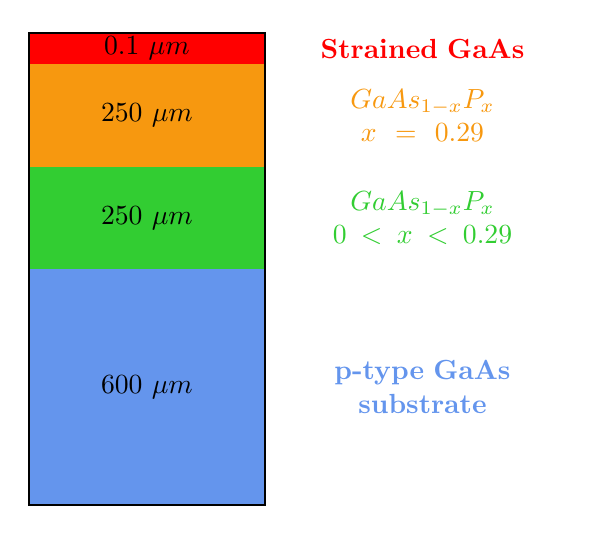
\begin{tikzpicture}
	    \tikzstyle{explain} = [align=center] 
	    \centering
	    \fill [CornflowerBlue] (0, 0) rectangle (3, 3);
	    \node at (3/2, 3/2) {\bm{$600 \ \mu m$}};
	    \node [explain, CornflowerBlue, text width=3.4 cm] at (5, 3/2) {\textbf{p-type GaAs substrate}};
	    \fill [LimeGreen] (0, 3) rectangle (3, 3+1.3);
	    \node at (3/2, 3 + 1.3/2) {\bm{$250 \ \mu m$}};
	    \node [explain, LimeGreen, text width=3.5 cm] at (5, 3+1.3/2) {\bm{$GaAs_{1-x}P_x$} \\ \bm{$0 < x < 0.29$}};
	    \fill [YellowOrange] (0, 3+1.3) rectangle (3, 3+1.3+1.3);
	    \node at (3/2, 3 + 1.3 + 1.3/2) {\bm{$250 \ \mu m$}};
	    \node [explain, YellowOrange, text width=3.5 cm] at (5, 3+1.3+1.3/2) {\bm{$GaAs_{1-x}P_x$} \\ \bm{$x = 0.29$}};
	    \fill [Red] (0, 3+1.3+1.3) rectangle (3, 6);
	    \node at (3/2, 3 + 1.3 + 1.3 + 0.4/2) {\bm{$0.1 \ \mu m$}};
	    \node [explain, Red, text width=3.5 cm] at (5, 3+1.3+1.3+0.4/2) {\textbf{Strained GaAs}};
	    \draw [thick] (0, 0) rectangle (3, 6);
	    \label{fig:excitation-a}
	\end{tikzpicture}
    \end{subfigure}
    \hfill
    \begin{subfigure}[b]{0.49\textwidth}
	\centering
	\begin{tikzpicture}
	    \begin{axis}[axis lines=middle,
		xmin=0, xmax=8,
		ymin=0, ymax=7,
		xlabel={\large $m_j$},
		ylabel={\large$E$},
		xlabel style={above},
		xtick=\empty,
		ytick=\empty,
		]
		\draw [/pgfplots/every inner y axis line, draw=black] (6.5,0) -- (6.5, \pgfkeysvalueof{/pgfplots/ymax}) node [below right] {\large J}; 
		\draw [draw=Violet, line width=2pt] (1.25,\yone) -- (2.25, \yone) node [midway, below, Violet] {\textbf{-1/2}};
		\draw [draw=Violet, line width=2pt] (4.25,\yone) -- (5.25, \yone) node [midway, below, Violet] {\textbf{+1/2}};
		\draw [draw=OliveGreen, line width=2pt] (0.5,\ytwo) -- (1.5, \ytwo) node [midway, below, OliveGreen] {\textbf{-3/2}};
		\draw [draw=OliveGreen, line width=2pt] (2,\ytwo-0.5) -- (3, \ytwo-0.5) node [midway, below, OliveGreen] {\textbf{-1/2}};
		\draw [draw=OliveGreen, line width=2pt] (3.5,\ytwo-0.5) -- (4.5, \ytwo-0.5) node [midway, below, OliveGreen] {\textbf{+1/2}};
		\draw [draw=OliveGreen, line width=2pt] (5,\ytwo) -- (6, \ytwo) node [midway, below, OliveGreen] {\textbf{+3/2}};
		\draw [draw=Blue, line width=2pt] (2,\ythree) -- (3, \ythree) node [midway, above, Blue] {\textbf{-1/2}};
		\draw [draw=Blue, line width=2pt] (3.5,\ythree) -- (4.5, \ythree) node [midway, above, Blue] {\textbf{+1/2}};
		\node [Violet, right] at (6.7, \yone-0.1) {\large\bm{$P_{1/2}$}};
		\node [OliveGreen, right] at (6.7, \ytwo-0.1) {\large\bm{$P_{3/2}$}};
		\node [Blue, right] at (6.7, \ythree-0.1) {\large\bm{$S_{1/2}$}};

		\draw [-stealth, Red, line width=2pt] (1, \ytwo) -- (2.5, \ythree) node [above, midway, sloped] {\bm{$\sigma^+$}};
		\draw [-stealth, YellowOrange, line width=2pt] (5.5, \ytwo) -- (4, \ythree) node [above, midway, sloped] {\bm{$\sigma^-$}};
	    \end{axis}
	\end{tikzpicture}
	\label{fig:excitation-b}
    \end{subfigure}
    \caption{Strained GaAs}
\end{figure}

%%%%%%%%%%%%%%%%%%%%%%%%%%%%%%%%%%%%%%%%%%%%%%%%
\subsection{Polarization Control}
\begin{figure}[h!]
    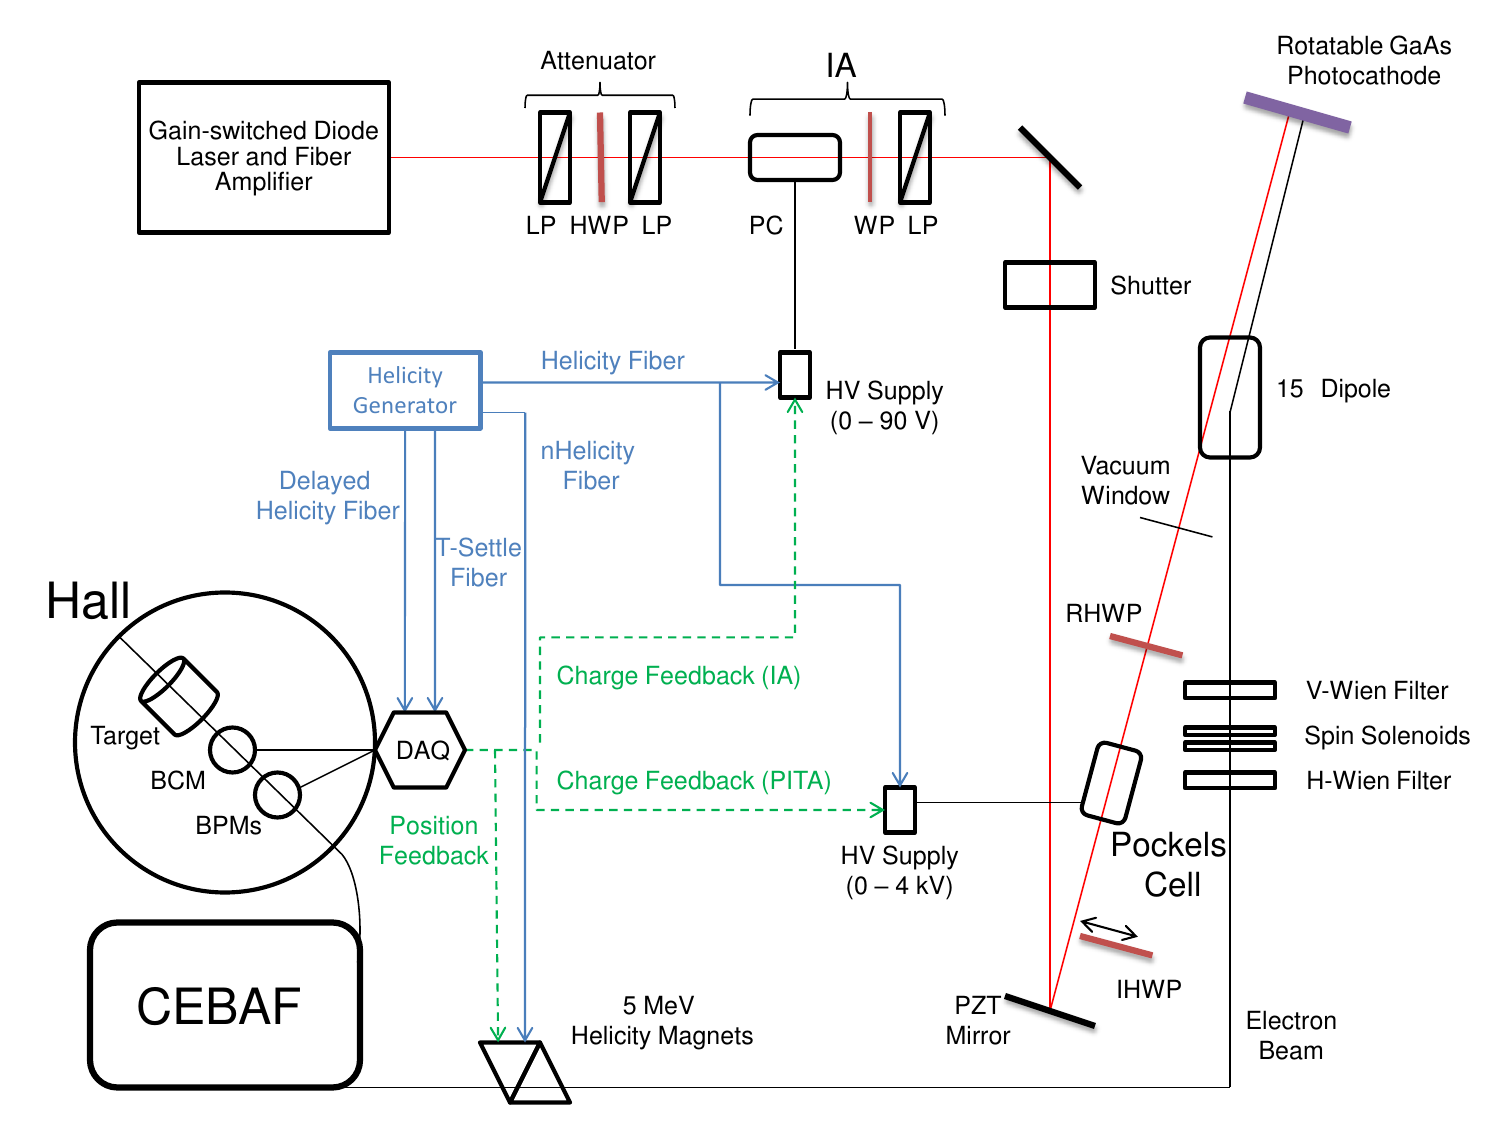
\includegraphics[width=\linewidth]{injector}
    \caption{The laser system at the CEBAF injector}
    \label{fig:injector}
\end{figure}

\begin{figure}[h!]
    \begin{tikzpicture}
	\tikzstyle{explain} = [align=center] 
	\begin{scope}
	    \node[anchor=south west, inner sep=0] (image) at (0, 0)
	    {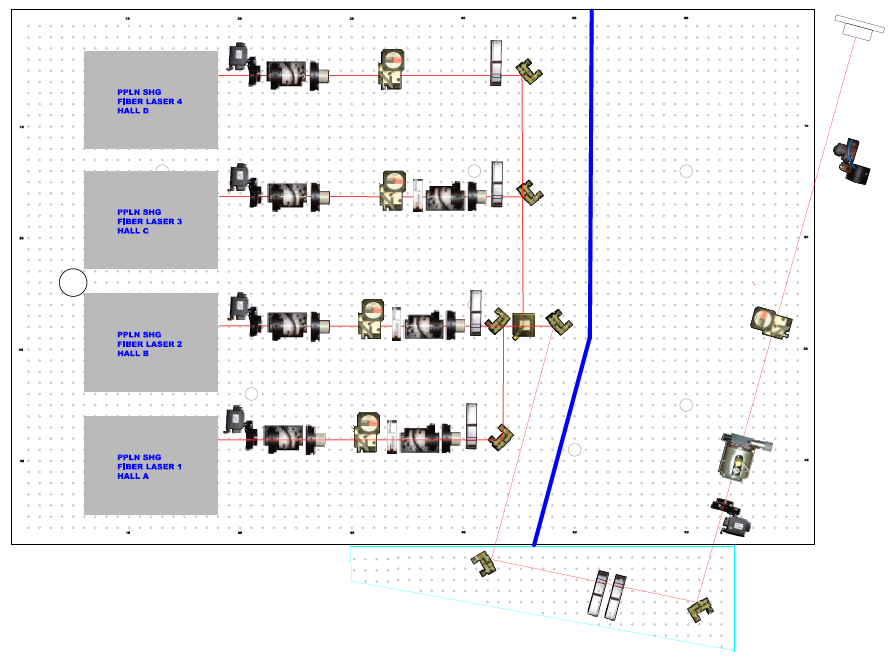
\includegraphics[width=\linewidth]{laser_table}};
	    \begin{scope}[x={(image.south east)},y={(image.north west)}]
		\node [blue,ultra thick] at (0.06,0.3) {\textbf{A}};
		\node [blue,ultra thick] at (0.06,0.49) {\textbf{B}};
		\node [blue,ultra thick] at (0.06,0.67) {\textbf{C}};
		\node [blue,ultra thick] at (0.06,0.85) {\textbf{D}};

		\node [blue,ultra thick] at (0.47,0.39) {\textbf{IA}};
		\node [blue,ultra thick] at (0.47,0.56) {\textbf{IA}};
		\node [blue,ultra thick] at (0.5,0.75) {\textbf{IA}};

		\node [red] at (0.75,0.23) {\textbf{IHWP}};
		\node [explain,red] at (0.76,0.33) {\textbf{Pockels } \\ \textbf{Cell}};
		\node [red] at (0.78,0.52) {\textbf{RHWP}};
		\node [explain,red] at (0.88, 0.96) {\textbf{Beamline} \\ \textbf{vaccum} \\ \textbf{window}};
	    \end{scope}
	\end{scope}
    \end{tikzpicture}
    \caption{How the laser table actually looks like}
    \label{fig:laser_table}
\end{figure}

%%%%%%%%%%%%%%%%%%%%%%%%%
\subsubsection{Pockels Cell}
Now that we can produce polarized electron beams, we need more control over the
polarization of the electron beams. We should be able to flip the beam polarization
quickly while keeping polarization as stable as possible. It is not easy and time
consuming to manipulate the electron directly, while manipulating photons is much 
easier. One just need to reverse the circular polarization of the laser pulse,
it will flip the electron beam polarization. The easiest way to do the job is
a half-wave plane, by inseting in into or retracting it from the laser path,
the phase of the laser pulse will be changed by $\pi$, flipping the laser
circular polarization. But mechanical movement is not fast enough, the fast 
flipping of beam polarization is done by a component called Pockels Cell (PC),
which is Rubidium Titanyle Phosphate (RTP) crystal. PC operates based on the 
Pockels effect, which is the production of birefringence in the crystal under
an electric field, the birefringence is proportional to the strength of the
applied electric field. By applying appropriate high voltage ($\sim 1.5\ kV$),
% from Caryn's thesis
PC will act as a quarter wave plate (photon amplitude along fast and low axes
$E_x$, $E_y$ will have a phase difference of $\pm \frac{\pi}{2}$ dependeing on
the polarity of the applied electric field), converting lineraly polarized laser beam
into circularly polarized laser beam. And reserve the electric field polarity
will reverse the polarization of the laser beam. This transition can be very
fast, up to $1 \ kHz$, with a dead time of about $60\ \mu s$.
% Moller will go up to 2 kHz, with 10 \mu s settle time

\subsubsection{Polarization Induced Transport Asymmetry (PITA, or Phase Induced Transmission Asymmetry) \cite{Cary2019}}
What we talked about above is the ideal case that PC will be an exact quarter wave
plate and other optical components also work well, in reality, there is always 
deviation from the perfect circular polarization,
resulting in systematic effect on beam position, spot size and intensity. If the deviation 
is polarization correlated, it will introduce a false asymmetry to our PV asymmetry 
measurement, which is called the PITA effect. The PITA effect is the dominant
piece of HCBA, which, as we said before, is the largest false asymmetry in
our measurement.

\begin{figure}[h!]
    \centering
    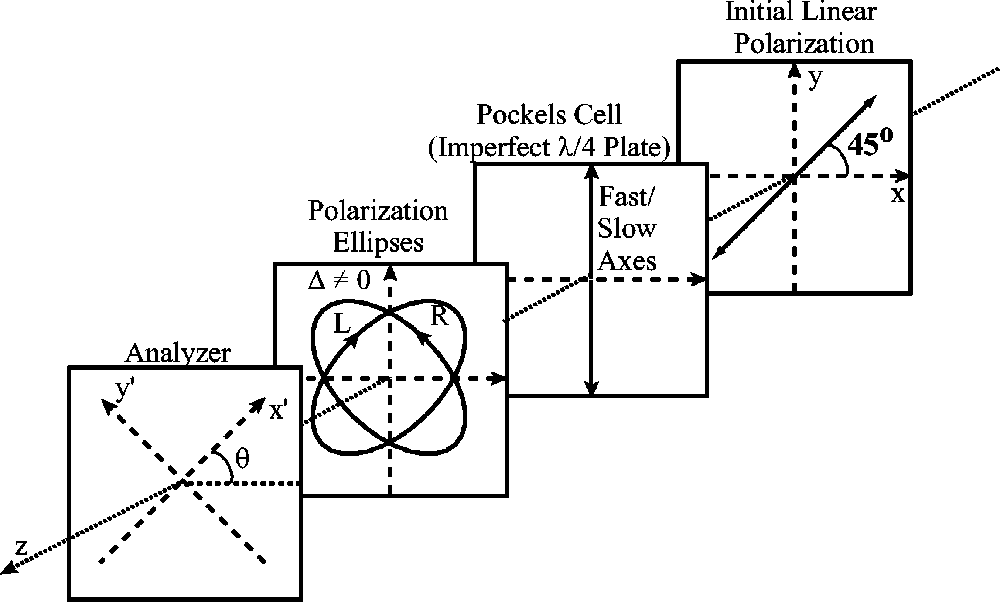
\includegraphics[width=0.6\linewidth]{PC_phase_shift}
    \caption{Phase shift by going through the PC}
    \label{fig:pc_phase_shift}
\end{figure}

The PITA effect is characterized by the PC induced phase shift $\delta$
\begin{equation*}
    \delta^{R(L)} = \mp\left(\frac{\pi}{2} + \alpha \right) - \Delta \\
\end{equation*}
where $\alpha$ and $\Delta$ represnet the symmetric and asymmetric offset phase
shift respectively. The resultant slightly elliptical beam has a residual
linear component, leading to an intensity asymmetry (to first order):
\begin{equation}
    \CA_{I} = \frac{I^R - I^L}{I^R + I^L} = -\frac{\epsilon}{T}[\Delta\cos(2\theta)]	\\
\end{equation}
$\epsilon/T \ (<<1)$ defines the ``analyzing power'', $\epsilon = T_{x'} - T_{y'}$ 
and $T = (T_{x'} + T_{y'})/2$,
$T_{x' (y')}$ is the transimission coefficient along the axis x' (y') of the
downstream analyzer. $\theta$ is the angle between the PC's fast axis and the 
$x'$ axis of the analyzer

Consider other optical elements along the laser path, like the RHP and the vacuum
window, the unknown tiny birefringence in these components will also contribute to $\Delta$,
resulting to a modified intensity asymmetry:
\begin{equation}
    \CA_{I} = \frac{I^R - I^L}{I^R + I^L} = -\frac{\epsilon}{T}[\cos(2\theta)\cdot(\Delta - \Delta^0)]	\\
\end{equation}

To minimize the intensity asymmetry, one would like to keep $\Delta - \Delta^0$
as small as possible. Fortunately, $Delta$ is tunable, by change the applied
electric field. As shown in fig. \ref{fig:injector}, our charge feedback system
will monitor the charge intensity asymmetry and automatically adjust the HV 
supplied to the PC to maintain a small $\CA_I$. Over CREX, the average charge
intensity asymmetry is ??? ppm.

As you may see in fig. \ref{fig:injector}, the charge feedback system also
controls the HV supply of the Intensity Attenuator (IA), which, together with
the slit in beam chopper, controls the intensity of electron beams. So, IA also
plays a key role in achieving a small charge intensity asymmetry by eqaulizing
beam intensity across helicity states.

A optical element called Rotatable Half-Wave Plate (RHWP) lies downstream the PC,
it help to equalize any residual linear polarization left in the PC to establish 
a Quantum Efficiency (QE) independence of helicity.

\subsubsection{Slow Helicity Reversal}
Fast reversal of the PC can minimize a lot of random noise from beam and target
density fluctuations, nevertheless, some helicity correlated (HC) false asymmetries
remain, such as electronic pickup between accelerator electronic systems and 
the experimental DAQ system or the residual birefringence effect. It is the 
job of slow helicity reversal to cancel these systematic false asymmetries.

There are 2 methods to make slow helicity reversal -- the Insertable Half-Wave Plate (IHWP) 
and the double Wien Filters. Prior to 2009, IHWP was the only available approach
at CEBAF to do slow helicity reversal. A new mechanism was introduced during 
PREX-I and Qweak experiments for better systematic precision -- the wien filter.

The IHWP lies upstream of the PC, it is the easiest way to reverse the beam 
helicity by inserting or retracting the IHWP. With slow helicity reversal, we 
can identify the possible systematic undertainties. The idea
is simple, assume the true and a systematic false asymmetry to be $A_0$ and $\Delta A$,
then what we measure by inserting (retracting) the IHWP will be:
\begin{equation}
    A^{+(-)} = \pm A_0  + \Delta A
\end{equation}
Because IHWP doesn't affect the systematic uncertainty, so the true asymmetry
will be:
\begin{equation}
    A_0 = \frac{A^+ - A^-}{2}
\end{equation}

As easy and good as IHWP, it resolves only some of the HC beam variations, namely
the residual birefringence from the laser optical system and is powerless in dealing
with other HC effects, like HC beam size variations that are introduced via
PC focusing \cite{osti_1059486}, which is addressed by the wien filter.
The wien filter manipulate the electron spin directly by electromagnetic field 
without affecting the electron movement and is able to achieve any spin orientation.
It consists of 2 wien filters and 2 intervening solenoids between them.
A wien filter is such a cavity with proper electric and magnetic field ($qE = qvB$), 
perpendicular to each other and to the electron moving direction, so that it 
rotates electron spin only.
Electrons coming from the photocathode are longitudinally polarized,
the vertical wien filter will make the electron spin vertical oriented, so that
it can be rotated to left/right by the following spin solenoid, depending on
the polarity of the solenoid, a wien flip means to change the polarity of the spin solenoid.
Finally, the horizontal wien filter will fine tune the spin direction to optimize 
the longitudinal polarization in the experimental hall. Note that electrons
exit the double wien filters are not longitudinally polarized, because electron
spin will precess when travel through the accelrator, causing a rotation in the
horizontal plane. Therefore, a carefully selected initial spin direction is 
needed to make sure the spin is (anti) parallel to electron momentum at target.
\begin{figure}
    \centering
    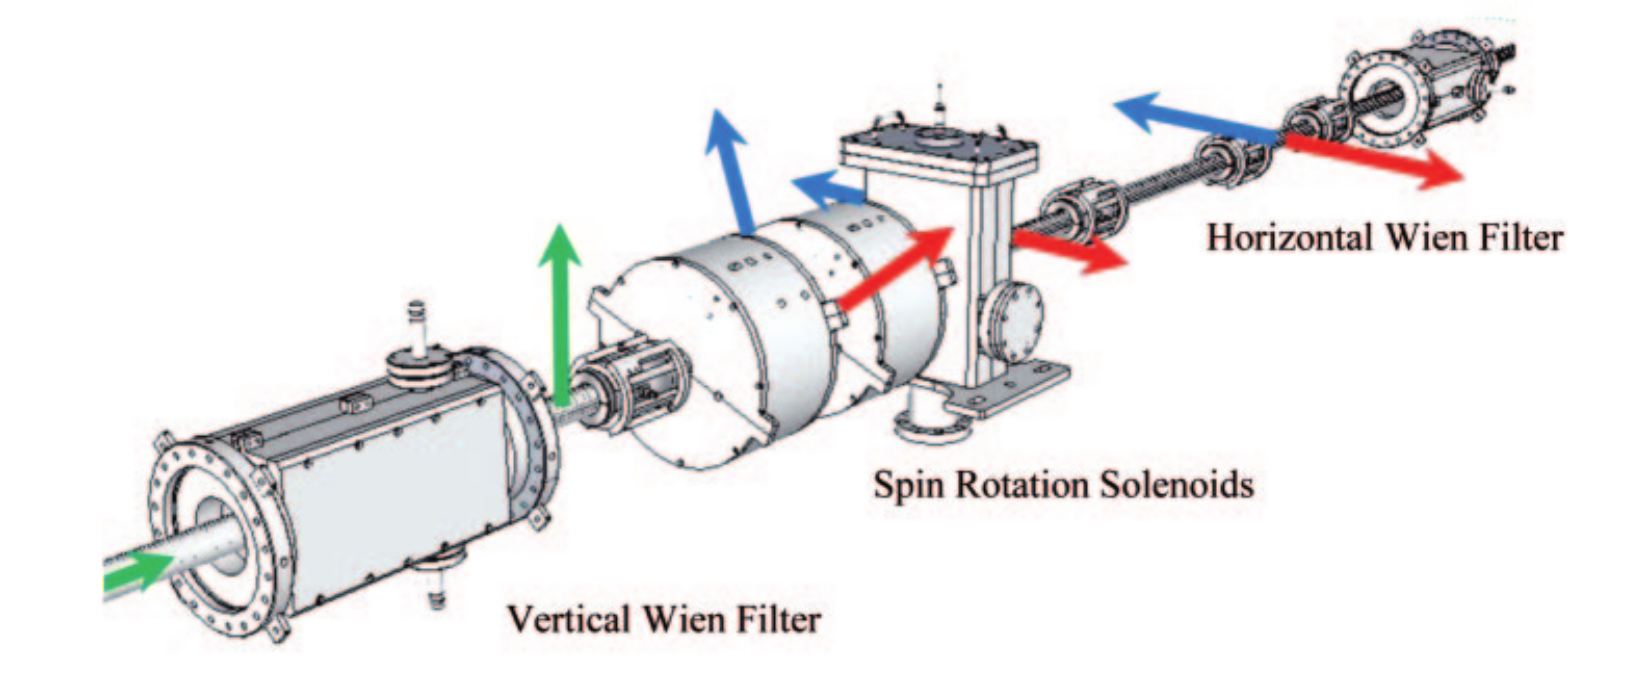
\includegraphics[width=0.6\linewidth]{wien_filter}
    \caption{Schematic plot of double wien filter, electron beam travels from left
    to right. \cite{osti_1059486}}
\end{figure}

This tells us another function of the wien filter, to set a non-longitudinal 
initial spin to cancel out the shift caused by spin precession during acceleration, 
so that we have exactly longitudinally polarized electron beam at target.

With both IHWP and Wien filter, we are able to cancle most systematic false 
asymmetries, achieving very small systematic errors.

%%%%%%%%%%%%%%%%%%%%%%%%%%%%%%%%%%%%%%%%%%%%%%%%
\subsection{Polarimeters}
Now that we have polarized electron beams, we still need to measure its polarization.
We have 3 polarimeters to measure the beam polarization: the Mott polarimeter
at injector and the Compton and Moller polarimeter in Hall A. As their names
imply, they use the cross section asymmetry of the Mott, Compton and Moller
scattering to measure the polarization of the electron beam. Since these are
all pure QED processes, their cross sections are well understood and analyzing 
powers are easily calculable to high order.

While both Mott and Moller measurement are invasive, they can't be done frequently
(Moller measurement happens about every 10 days).
the non-invasive Compton polarimeter is the only choice for beam polarization monitoring. 
Mott polarimeter measures the beam polarization before it enters the accelerator, 
so it is not used for the determination of beam polarization during PREX-II/CREX.

%%%%%%%%%%%%%%%%%%%%%%%%
\subsubsection{Mott Polarimeter}
\begin{figure}
    \centering
    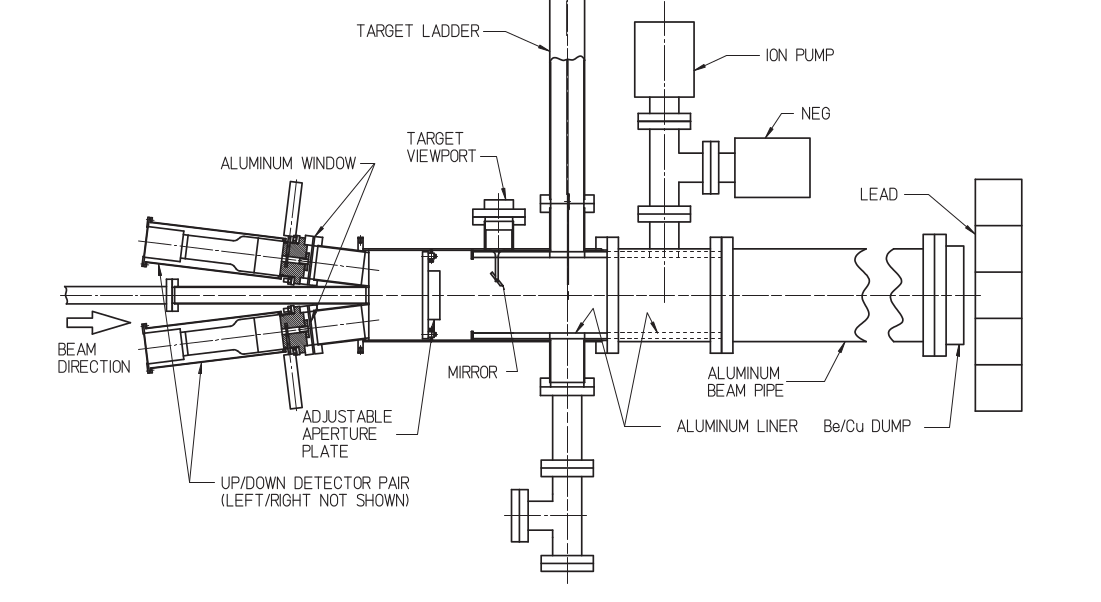
\includegraphics[width=0.6\linewidth]{Mott_polarimeter}
    \caption{Schematic plot of the Mott polarimeter, it has 4 symmetric detector
    ports (up and down, left and right -- which is not shown in the plot). 
    The back scattering angle is $172.6^\circ$, where we have the
    highest analyzing power from theoretical calculation of the Sherman function.
    \cite{PhysRevC.102.015501}}
\end{figure}
The 5-MeV Mott polarimeter lies at the CEBAF injector, between the Wien Filter
and the Injection Chicane, it measures the single spin cross section asymmetry
of $5\ MeV$ electron beams scattered off a high-Z target. Comparing the measurement
to the Sherman Function \cite{PhysRev.103.1601}, the analyzing power, will tell
us the transverse polarization of the electron beam:
\begin{equation}
    \CA_{LR} = \frac{N_L - N_R}{N_L + N_R} = S(\theta)\vec{P}\cdot \hat{\vec{n}}
\end{equation}
$\hat{\vec{n}}$ is the unit normal vector of the scattering plane. The same formula
applies to the Up-Down asymmetry.
\begin{figure}
    \centering
    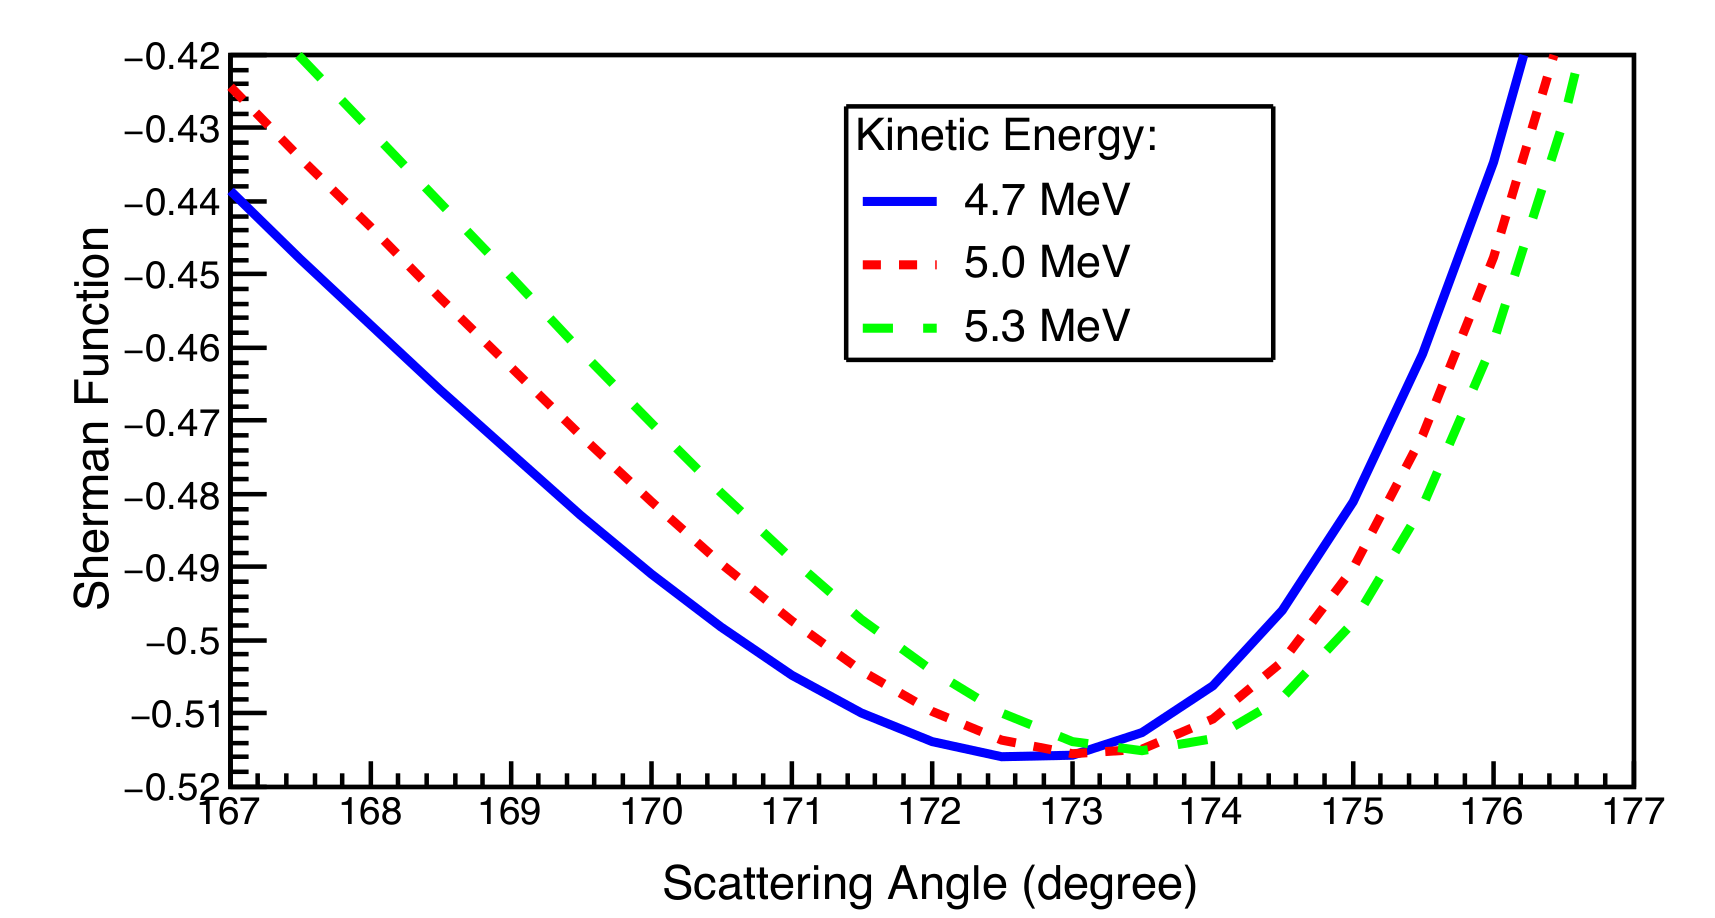
\includegraphics[width=0.6\linewidth]{Mott_asym}
    \caption{The Sherman Function for different high-Z targets at 5 MeV, dots
    represent experimental measurement.}
\end{figure}
Because the asymmetry comes from the coupling of electron's spin and the induced
magnetic field by the nucleus in the electron's rest frame (spin-orbit coupling), 
the scattering potential is:
\begin{equation}
    V(r, \vec{L}, \vec{S}) = V_{Coulomb} + V_{so} (r, \vec{L}, \vec{S}) = \frac{Ze}{r} + \frac{Ze^2}{2m^2r^3}\vec{L}\cdot \vec{S}
\end{equation}
So only transverse polarization can be measured using Mott polarimeter, rather
than the longitudinal one we desire at the target. Nevertheless, it provides an
independent check of the initial beam polarization from the injector and its high
precision (its total uncertainty can be as small as 0.61\% \cite{PhysRevC.102.015501}) 
helps to normalize the polarization measurement in the experimental halls.

%%%%%%%%%%%%%%%%%%%%%%%%
\subsubsection{Compton Polarimeter}
The Compton polarimeter locates at the entrance to hall A (about 20 m upstream the 
target chamber), using the elastic scatter between polarized photon and electron
to measured the polarization of the electron beam. As shown in fig \ref{fig:compton_pol},
when the compton polarimeter is on, the electron beam will be bent into the 
Compton Chicane to interact with the polarized photons nearly head-on (a tiny
crossing angle of $23.5\ mrad$). The Fabry-Perot Cavity
is locked to and filled with circularly polarized ($> 99\%$) green laser beam
($\lambda = 532\ nm$, $E = 2.334\ eV$).
The back-scattered photons will be
detected by a GSO (low energy) or $\text{PbWO}_4$ crystal calorimeter right of the interaction region, while the
electron beam will be bent back to the beam pipe to bombar the target. Due to
interaction with photons, the scattered electrons will be less energetic than
the incoming ones. So under the same dipole field, the scattered electrons will
be bent more than the non-interacting electrons, as shown by the red dash line 
in Fig. \ref{fig:compton_pol}. This 
seperation allow us to measure the scattered electrons, together with measurement
of scattered photons, we can identify and scattering asymmetry and then the polarization
of the electron beam.
\begin{figure}[h!]
    \begin{subfigure}[c]{0.55\linewidth}
	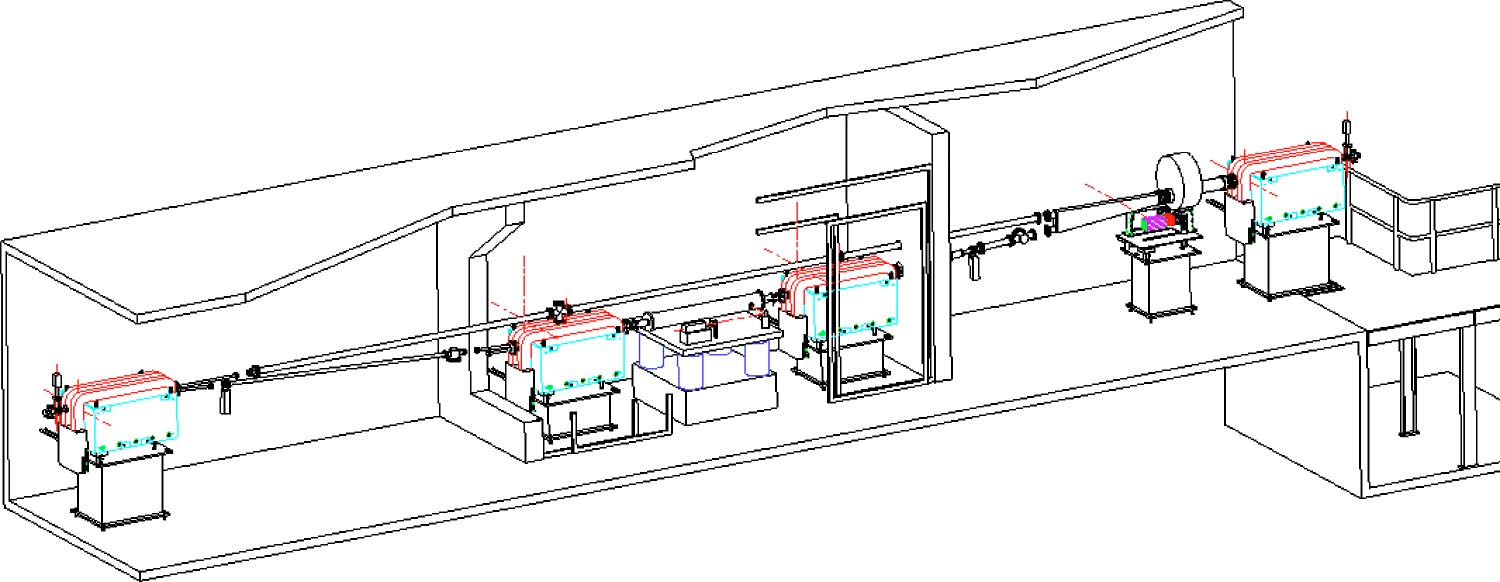
\includegraphics[width=\linewidth]{Compton_setup}
    \end{subfigure}
    \begin{subfigure}[c]{0.55\linewidth}
	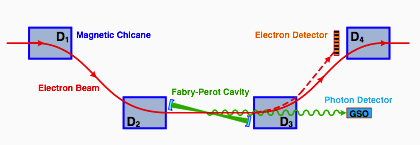
\includegraphics[width=\linewidth]{Compton_beam_path}
    \end{subfigure}
    \caption{Left: Compton Chicane \cite{PhysRevSTAB.7.042802}; 
    Right: Schematic plot of electron/photon scattering} 
    \label{fig:compton_pol}
\end{figure}

The energy of the scattered photon will be:
\begin{equation}
    E_\gamma \approx E_{laser} \frac{4a\gamma^2}{1 + a\theta^2_\gamma \gamma^2}
\end{equation}
where $\gamma = E_{beam}/m_e$ is the Lorentz factor of the incoming electron, 
$a = \frac{1}{1 + 4\gamma E_{laser}/m_e}$ and $\theta_\gamma$ is the scattering
angle w.r.t. the electron moving direction. The maximum energy of the scattered
photon appears at $\theta_\gamma = 0$, which is back scattering. 
For PREX-II (CREX) beam energy of $0.95\ (2.2)\ GeV$, $E_\gamma^{max} \sim 32.55 \ (167.02)\ MeV$.

Define $\rho = \frac{E_\gamma}{E_\gamma^{max}}$, the cross section for unpolarized
Compton scattering will be:
\begin{equation}
    \frac{d\sigma}{d\rho} = 2\pi r_0^2 a 
    \left[ \frac{\rho^2 (1-a)^2}{1 - \rho(1-a)} + 1 + \left( \frac{1 - \rho(1+a)}{1- \rho(1-a)}\right)^2\right]
\end{equation}
$r_0 = \frac{\alpha \hbar c}{mc^2}$ is the classical electron radius; then the
analyzing power will be:
\begin{equation}
    \CA_l = \frac{\sigma^\rightarrow_\Rightarrow - \sigma^\leftarrow_\Rightarrow}
    {\sigma^\rightarrow_\Rightarrow + \sigma^\leftarrow_\Rightarrow}
    = \frac{2\pi r_0^2 a}{d\sigma/d\rho}(1 - \rho(1+a))\left[ 1 - \frac{1}{(1 - \rho(1-a))^2}\right]
\end{equation}
\begin{figure}
    \centering
    \includegraphics[width=0.5\linewidth]{compton_asym}
    \caption{The Compton analyzing power increases with electron energy. Note
    that the analyzing power will change sign at $\rho \sim 0.5$ for both PREX-II
    and CREX beam energies.}
\end{figure}

The measured asymmetry will be:
\begin{equation*}
    \CA_{\text{exp}} = \CP_{e}\CP_{\gamma}\CA_{l} = \frac{N_{\gamma}^R - N_{\gamma}^L}{N_{\gamma}^R + N_{\gamma}^L}
    \Rightarrow
    \CP_e = \frac{\CA_{\text{exp}}}{\CP_{\gamma}\CA_{l}}
\end{equation*}
The advantage of the Compoton polarimeter is that it can tolerate quite high current
(up to $\sim 200 \ \mu A$ at JLab), plus its non-invasive operation make it a beam 
polarization monitor. The disadvantage is, comparing to Mott or Moller polarimeter,
its analyzing power is quite low at GeV energy level, while increase the beam
energy will lead to high background in the photon detection due to synchrotron 
radiation. Overall, the Compton polarimeter is able to achieve a 1\% absolute systemtatic
uncertainty.

%%%%%%%%%%%%%%%%%%%%%%%%
\subsubsection{Moller Polarimeter}
\begin{comment}
low current only
\end{comment}

The Moller polarimeter lies downstream of the Compton polarimeter and upstream 
of the target chamber. It uses elastic electron-electron scattering to measure the
asymmetry due to different beam polarizations. 
\begin{equation}
    \begin{gathered}
	\frac{d\sigma}{d\Omega} = \frac{d\sigma_0}{d\Omega} (1 + \sum_{i,j=x,y,z} \CP_b^i \cdot \CP_t^j \cdot A_{ij}(\theta_{CM})) \\
	\frac{d\sigma_0}{d\Omega} = \frac{\alpha^2}{s} \left( \frac{4 - \sin^2\theta_{CM}}{\sin^2\theta_{CM}}\right)^2 
    \end{gathered}
    \label{eqn:moller_xsection}
\end{equation}
With $frac{d\sigma_0}{d\Omega}$ being the unpolarized moller scattering cross section,
s is the Mandalstam variable: $s = 2m_e(E+m_e) \approx 2m_e^2\gamma$,
$\CP_b \ (\CP_t)$ the polarization of beam (target). 
$\theta_{CM}$ and $A_{ij}$ the scattering angle and analyzing power in CoM frame. 

Assuming incoming electrons move in the z direction and the scattering happens
in the xz plane, then in the ultra-relativistic limit:
\begin{equation}
    \begin{gathered}
	A_{zz} = \frac{\sin^2\theta_{CM} (7 + \cos^2\theta_{CM})}{(3+\cos^2\theta_{CM})^2},
	\quad
	A_{xx} = -A_{yy} = \frac{\sin^4\theta_{CM}}{(3+\cos^2\theta_{CM})^2}	\\
	A_{xz} = A_{zx} = \frac{2\sin^4\theta_{CM}\cos\theta_{CM}}{\gamma(3+\cos^2\theta_{CM})^2},
	\quad
	A_{xy} = A_{yz} = A_{yz} = A_{zy} = 0
    \end{gathered}
\end{equation}
When $\theta_{CM} = 90^\circ$, $A_{zz}$ is maximized to be $\frac{7}{9}$. This
is what we choose in the moller polarimeter.

The polarized target electrons come from magnetized Fe-alloy foil, which is 
saturated by a very strong ($4\ T$) longitudinal magnetic field created by 
superconducting Helmholtz coils, as shown in Fig. \ref{fig:moller_polarimeter}. 
So Eq. \ref{eqn:moller_xsection} is simplified to:
\begin{equation}
    \frac{d\sigma}{d\Omega} = \frac{d\sigma_0}{d\Omega} ( 1 + \CP_b^z \cdot \CP_t^z \cdot A_{zz}(\theta_{CM}))
    \label{eqn:moller_xsection_1}
\end{equation}
The moller pair (the scattered incident electrons and recoil target electron)
centered around $\theta_{CM} = 90^\circ$ ($\theta_{lab} < 3^\circ$), 
are seperated from the undeflected beam by set of magnets, then goes through
collimators (at the exit of dipole, not shown in Fig. \ref{fig:moller_polarimeter}) 
that define the acceptance, and finnally is detected by electron detectors in coincidence.
The measreud asymmetry between spin-parallel and anti-parallel cross section is:
\begin{equation}
    A_{exp} = \frac{N^+ - N^-}{N^+ + N^-} = \CP_b \CP_t \langle A_{zz} \rangle 
    \Rightarrow
    \CP_b = \frac{A_{exp}}{\CP_t \langle A_{zz} \rangle}
\end{equation}
with $\langle A_{zz} \rangle$ being the average analyzing power over the acceptance,
which was about 0.75 for PREX-II and CREX.

% https://prex.jlab.org/DocDB/0005/000502/002/CREX_Moller_Polarimetry_Systematics_Oct_2021.pdf
The target foil was cooled by conduction through the target, whose temperature 
will climb quickly with increase beam current, causing damage to target
polarization. Therefore moller polarimeter can only operate at very low current ($\sim \mu A$).
The extrapolation from polarization measurement at low current to high current
where PREX-II and CREX run at, is a large source of systematic uncertainty.
During PREX-II and CREX, the target polarization was measured to be $\CP_t \sim 8\%$ 
leading to an effective analyzing power of $A_{eff} = \CP_t\langle A_{zz} \rangle = 6\%$.
This relative large analyzing power makes moller measurement quite precise.
Overall, Moller polarimeter in Hall A can achieve a systematic uncertainty less
than 1\%.

\begin{figure}[h!]
    \centering
    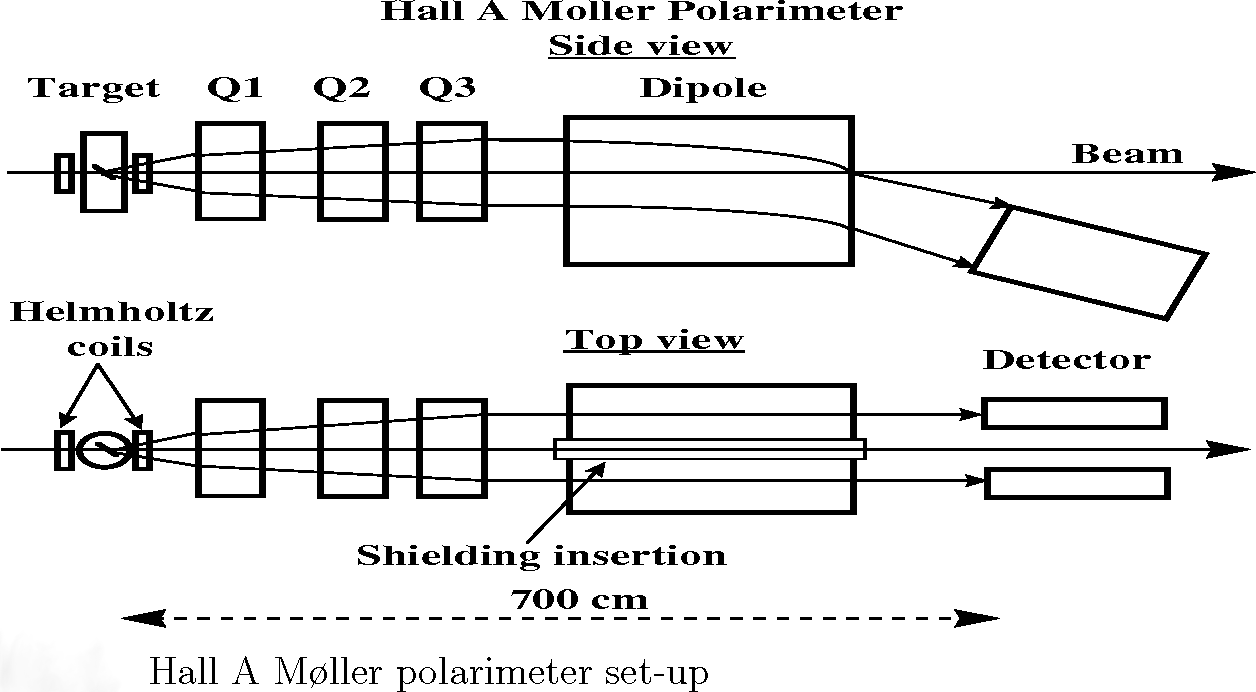
\includegraphics[width=0.7\linewidth]{moller_setup}
    \caption{Moller Polarimeter}
    \label{fig:moller_polarimeter}
\end{figure}

%%%%%%%%%%%%%%%%%%%%%%%%%%%%%%%%%%%%%%%%%%%%%%%%%%%%%%%%%%%%%%%%%%%%%%%%
\section{Monitors}
Besides beam polarization, another significant source of systematic uncertainty
is the beam false asymmetry -- the difference in beam position, angle, energy and
current between different helicity states. Because there is no way to ensure
exactly the same beam parameters between different helicity states, even with fast
helicity flipping. We monitored these variables with redundant specialised devices
-- Beam Position Monitors (BPMs) and Beam Current Monitors (BCMS). For PREX-II
and CREX, we had another independent monitor system -- Small Angle Monitors (SAms).
There monitors were able to measure the beam difference as precise as:
$$ \Delta x \sim 1\ \mu m \quad \Delta x' \sim 1\ mrad \quad \Delta p/p \sim 0.0004 \quad \Delta I/I \sim 100 \ ppm$$ (FIXME)
\begin{figure}[h!]
    \centering
    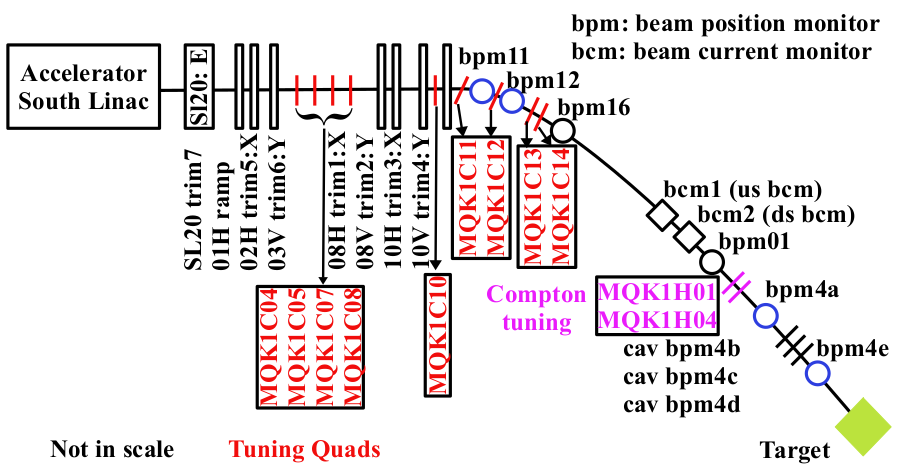
\includegraphics[width=0.6\linewidth]{beam_monitor_and_modulation}
    \caption{Schematic plot of Hall A beam monitor system and beam modulation system}
    \label{fig:hall_a_monitors_and_modulation}
\end{figure}

%%%%%%%%%%%%%%%%%%%%%%%%%%%%%%%%%%%%%%%%%%%%%%%%
\subsection{BPMs}
\begin{comment}
Cross check, and unfold beam fluctuation noise from instrumentation noise
\end{comment}
Hall A has a series of BPMs along the beam piple leading to the target chamber
to monitor the beam conditions, among them, 6 switchec electrode electronics (SEE) 
stripline BPMs are important to PREX-II and CREX, 
their records are used to extract beam parameters. These 6
key BPMs are shown in Fig. \ref{fig:hall_a_monitors_and_modulation}. 
BPM4A and BPM4E locate $7.524\ m$ and $1.286\ m$ upstream of the target chamber, 
they are used to determine the beam position and angle on the target. BPM11 and BPM12
are positioned on the arc area to measure the beam energy using the bending 
radius of the electron trajectory. BPM1 and BPM16 are backup monitors.

A stripline BPM consists of a 4-wire antenna array of open ended thin wire striplines, 
the voltage induced by the electron bunches in each electrode is sensitive to beam position.
Therefore we can extract (x', y') positions from opposite 2 pickup signals.
\begin{figure}
    \centering
    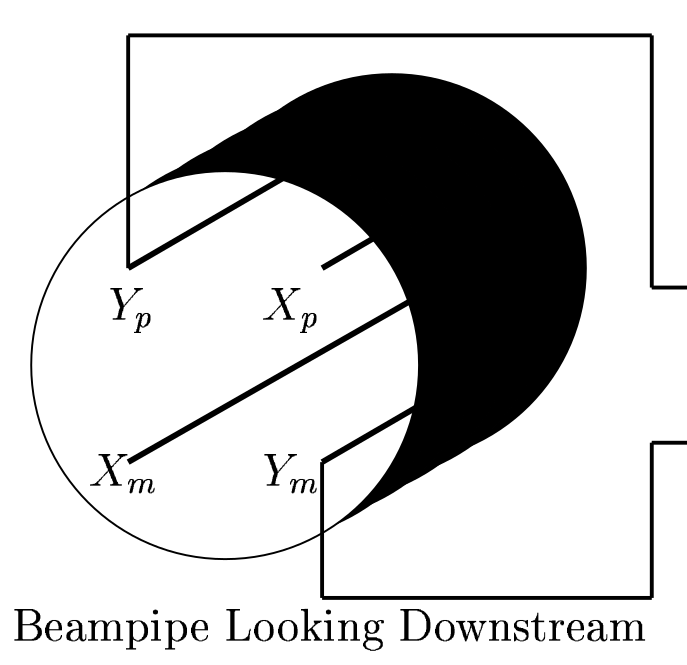
\includegraphics[width=0.4\linewidth]{stripline_bpm}
    \caption{Schematic plot of stripline BPM}
\end{figure}
\begin{equation}
    x' = \frac{1}{S_x} \frac{X_p - X_m}{X_p + X_m}   \\
    y' = \frac{1}{S_y} \frac{Y_p - Y_m}{Y_p + Y_m}   
\end{equation}
where the proportional constant $S_x$ ($S_y$) is the position sensitivity. 
The pickup voltage responds linearly to beam displacement when the displacement
is small. In the case of Hall A BPMs, the 4 striplines are rotated $45^\circ$
w.r.t. to hall coordinate system, so a $45^\circ$ rotation is needed to recover
hall (x, y) from extracted BPM (x', y').

Besides these stripline BPMs, PREX-II and CREX also utilized 3 cavity BPMs (see discussion below),
shown as bpm4b/c/d between bpm4a and bpm4e in Fig. \ref{fig:hall_a_monitors_and_modulation},
to measure beam conditions for low current calibration runs, because stripline
BPMs don't work when beam current is lower than $0.5\ \mu A$. These cavity
BPMs were not used in normal production runs.

%%%%%%%%%%%%%%%%%%%%%%%%%%%%%%%%%%%%%%%%%%%%%%%%
\subsection{BCMs}
One technique to measure beam current is current transformation.
Various BCMs based on this idea may have different designs, features and performances, 
the key component is the same -- current transformer (CT). When beam bunch 
travel through the beam pipe, it will induce a magnetic field in the beam pipe (the core), 
which in turn will induce a current in the secondary winding (toroid), 
whose output is proportional to the beam current. 
To make a precise measurement, it is important to shield any outside magnetic 
field and seperate the segment of beam pipe where the BCM lies in from the rest.

The BCM system in Hall A consists of two radio frequency (rf) cavities and
an unser monitor in between, the unser monitor is a parametric current transformer (PCT),
which will output a DC voltage equivalent to $4\ mV$ per $\mu A$ of beam \cite{987367}.
% With good magnet shielding, the unser monitor is able to measure the beam current
% at a precision of ???.
In PREX-II and CREX, the Unser monitor was not used for beam current measurement,
because its voltage output drifted quickly after only a few minutes of running,
instead, it was used to calibrate the rf-cavity monitors on either side of it,
whose readout was what we used for runtime beam current measurement.
\begin{figure}
    \centering
    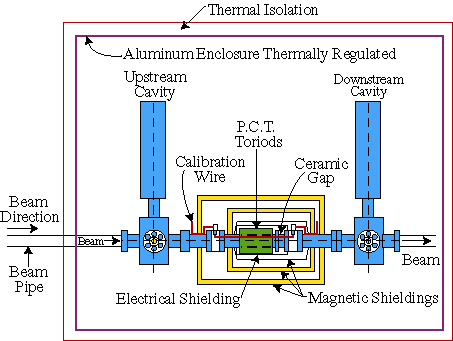
\includegraphics[width=0.5\linewidth]{bcm}
    \caption{Hall A BCM system \cite{987367}}
\end{figure}

A rf cavity is a metallic chamber that sustains an electromagnetic (EM) field 
(infinite number of resonant EM modes), by special design of its shape, a particular
EM mode can efficiently transfer energy to or from a charged particle. The 
frequently heard accelerating cavity need to provide a electric field along
beam velocity direction. While a decelerating cavity, which will absorb energy
from the coming charged particles, can be used as beam diagnostic monitors.
The induced voltage is proportional to the traversing charge q:
\begin{equation}
    V = 2k_{loss} q
\end{equation}
where $k_{loss}$ is the loss factor, which depends only on the electric field
distribution, therefore is sensitive to beam position and particle velocity.
To measure beam intensity, one would prefer the EM mode whose electric field
doens't depend on r position, these are $\text{TM}_{\text{010}}$ like modes;
while for measurement of beam position, exactly the opposite is wanted, the
electric field should have an azimuth angle and r dependence, which are $\text{TM}_{\text{110}}$
like modes.
\begin{figure}
    \centering
    \begin{subfigure}[c]{0.5\textwidth}
	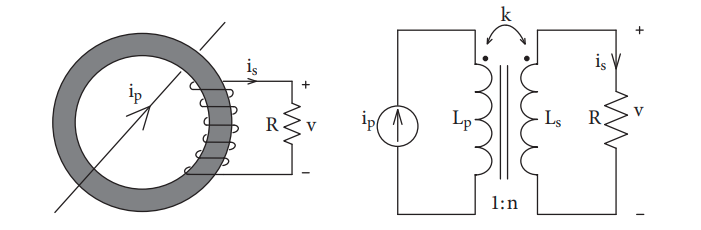
\includegraphics[width=\linewidth]{current_transformer}
    \end{subfigure}
    \begin{subfigure}[c]{0.55\textwidth}
	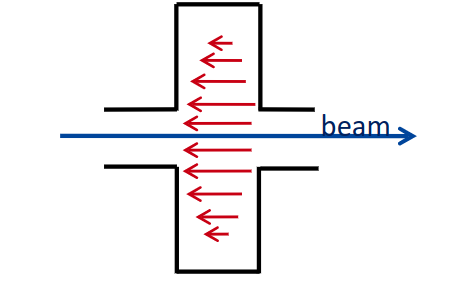
\includegraphics[width=0.52\linewidth]{TM010}
	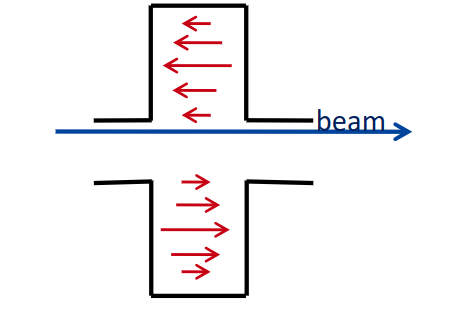
\includegraphics[width=0.46\linewidth]{TM110}
    \end{subfigure}
    \caption{Up: Schemtaic plot of current convertor; 
    Down: $\text{TM}_\text{010}$ and $\text{TM}_\text{110}$ modes, the red arrows are electric field}
\end{figure}

The 2 rf-cavity current monitors are of Pill box type (the electric field is
concentrated near axis, while the magnetic field is concentrated at outer
cylindrical wall), which operates at $\text{TM}_\text{010}$ mode. The voltage 
readout will be downconverted to lower frequencies signals, then filtered, 
amplified and further precessed before writing into the data stream. Due to
non-linearity at low current region, actually 3 signals (the same signal with
different gains: x1, x3 and x10) will be recorded \cite{hall_A_equip_manual}.

%%%%%%%%%%%%%%%%%%%%%%%%%%%%%%%%%%%%%%%%%%%%%%%%
\subsection{SAMs}
For further understanding of beam dynamics, electronic noise and possible target boiling
effect, a luminosity monitoring system, called the small angle monitors, was
installed in the dump pipe, about $7\ m$ downstream of the target pivot. As shown
in Fig. \ref{fig:sams}, the SAMs system consist of 8 detector modules, symmetrically 
positioned around the dump pipe. Each detector module has a quartz tile (active 
detector), attached to a lightguide, the Cherenkov light will be read out by a 
PMT at the end of the lightguide. 
As its name implies, SAMs are designed to monitor small angle ($\sim 1^\circ$)
scattered and secondary flux from the target, thus it can also be used to
inspect the target conditions, e.x. a bubble in the target that forms and disappears
within one helicity window is unknown to both BPMs and BCMs, but SAMs will see it.
SAMs' readout is sensitive to beam parameters,
e.x., the sum of a symmetric pair monitors is sensitive to change in beam current
and energy while their difference tells the fluctuation in beam position and angle.
The symmetric design helps to disentangle these beam parameters. So it provide
an independent check of the measurement of BPMs and BCMs and can be used to eliminate
possible beam or electronic noise.

\begin{figure}
    \centering
    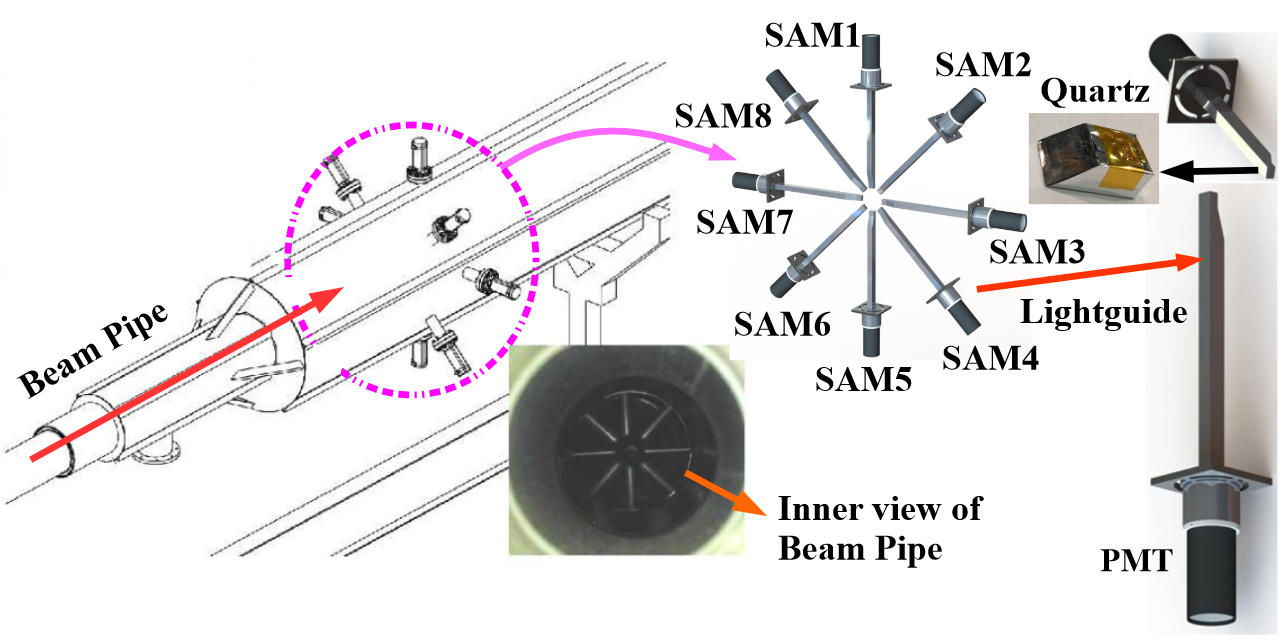
\includegraphics[width=0.8\linewidth]{sams_system}
    \caption{Layout of SAMs\cite{AJZ_thesis}}
    \ref{fig:sams}
\end{figure}

%%%%%%%%%%%%%%%%%%%%%%%%%%%%%%%%%%%%%%%%%%%%%%%%
\subsection{Beam Modulation}
\begin{comment}
It is very important for PVES to control the systematic uncertainty, especially
the one from beam fluctuation (HCBA). Ideally, the electrons bunches with opposite
polarization should have exactly the same internsity and energy, hitting the target 
at the same place with the same angle, which is obviously impossible in reality. 
So we need to correct the false asymmetry introduce by the beam fluctuation. There are a
few methods to do the correction, one of them is the so called Beam modulation.
The idea is to introduce man-made fluctuations to the beam through the 
modulation system, then we can measure the changes in monitors and detectors 
to find the sensitivities of detectors to changes in energy, position and angle,
which will be used to correct the measured asymmetry.
\end{comment}

Another system we see in Fig. \ref{fig:hall_a_monitors_and_modulation} is the
beam modulation system, which lies in beamline arc right after Beam Switch Yard 
where electron chains are seperate into Hall A/B/C beams.
It consists of 6 air-core coils and an energy vernier in the last cavity of south LINAC, 
the total number of 7 coils provides a redudancy w.r.t. the free number of degrees 
of beam phase space, making sure to cover all beam phase space at target.  
Coil (trim) 1, 3, 5 are responsible for modulating beam x position and coil 
2, 4, 5 will modulate beam y position.
These coils (vernier) are driven by a VME-DAC, which in turns is controlled by the parity DAQ.
It takes 4.267 s for each coil (vernier) to modulate the beam, a whole 
modulation cycle takes $85.68 \ s$ ($\sim 1$ beam modulation every 10 mins during
run time). 

The beam modulation system was used for false asymmetry correction, together with
regression. When beam was modulated, BPMs and detectors will record corresponding
change in their readout, to calculate detector sensitivity w.r.t. jitter in beam
parameters. Therefore, the modulation should be much larger than the natural
jitter in the beam, a typical position modulation will be about $100\ \mu m$ (FIXME)
and the energy vernier will result in a beam diplacement of $0.75 \ mm$ in BPM 11/12.
% \begin{figure}[h!]
%     \centering
%     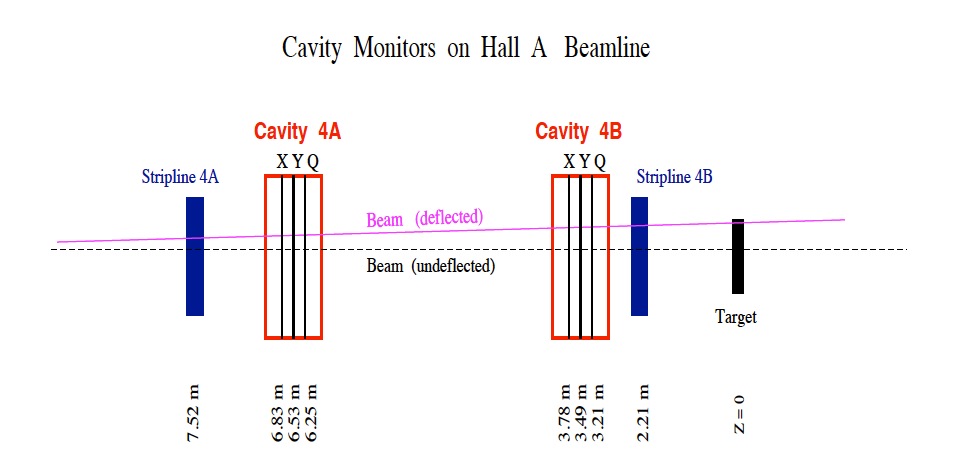
\includegraphics[width=0.49\linewidth]{bmw_modulated_beam}
% \end{figure}

%%%%%%%%%%%%%%%%%%%%%%%%%%%%%%%%%%%%%%%%%%%%%%%%%%%%%%%%%%%%%%%%%%%%%%%%
\section{Target}
For the sake of statistics, the designed current was quite large, as shown in
Table. \ref{table}. With such high current, the electron beam will deposit quite
a lot of heat on the target, it will be a disaster if we can't take away these
heat as soon as possible to keep a stable target temperature.
For PREX-II, because Pb itself is not a good thermal conductor ($35\ W/m\cdot K$),
auxiliary diamond foils ($> 1000\ W/m\cdot K$) were used to form a D-Pb-D sandwich target to help heat
dissipation. The thickness of the diamond foil matters, one lessen we learned 
from PREX-I was that with thin ($0.15\ mm$) diamond foil, the thermol conductivity
of the diamond foil droped greatly (from $1000 \ W/m \cdot K$ to $100 \ W/m\cdot K$) after about 
1 week of running with $70\ \mu A$ cw beam, resulting in some Pb targets melted. 
While a thicker diamond foil ($0.25\ mm$) will protect Pb foils from melting 
under the same conditions. In PREX-II, a factor of 2 safety margin was
adopted, conservatively assume 1 week running for each Pb target, 35 PAC days of beam time
requires 5 targets, and we deployed 10 isotopically pure Pb sandwich targets with 
thick diamond layers to ensure the success of PREX-II, each new target was able
to sustain up to $85\ \mu A$ cw beams.

While Ca itself is an excellent thermal conductor, no need for auxiliary 
materials and higher current can be applied. Isotopically pure \Ca (the original
target we used had a purity of 95.99\%) is much more 
expansive than pure \Pb target, so only one \Ca target was prepared for CREX. 
After the target accident, 
the new \Ca target was a stack of 3 seperated foils with similar total thickness.
% https://logbooks.jlab.org/entry/3769028

Targets were firmly mounted in bays of target ladders, whose axes were 
perpendicular to the beam line. The ladder was movable along its axis by an 
AC servo-motor, which can receive remote instructions through internet. 
The motion along ladder axis can be precise to $\sim12\ nm$.
% Thus each target foil would be placed at the same z position. 
There are 2 target ladders in total, one for production targets and the other
one for calibration targets. The production-ladder had 10 \Pb targets, 
two Calcium isotope targets: \ca and \Ca, and 4 other calibration and diagnostic
targets. The calibration-ladder holded a watercell, a thin C foil, a thin natural 
Pb and a thin \ca target.
The calibration-ladder was rotated $45^\circ$ w.r.t. the production ladder, 
which was along the lab x axis, as shown in Fig. \ref{fig:scattering_chamber}
and \ref{fig:target_ladder}.

\begin{figure}[h!]
    \centering
    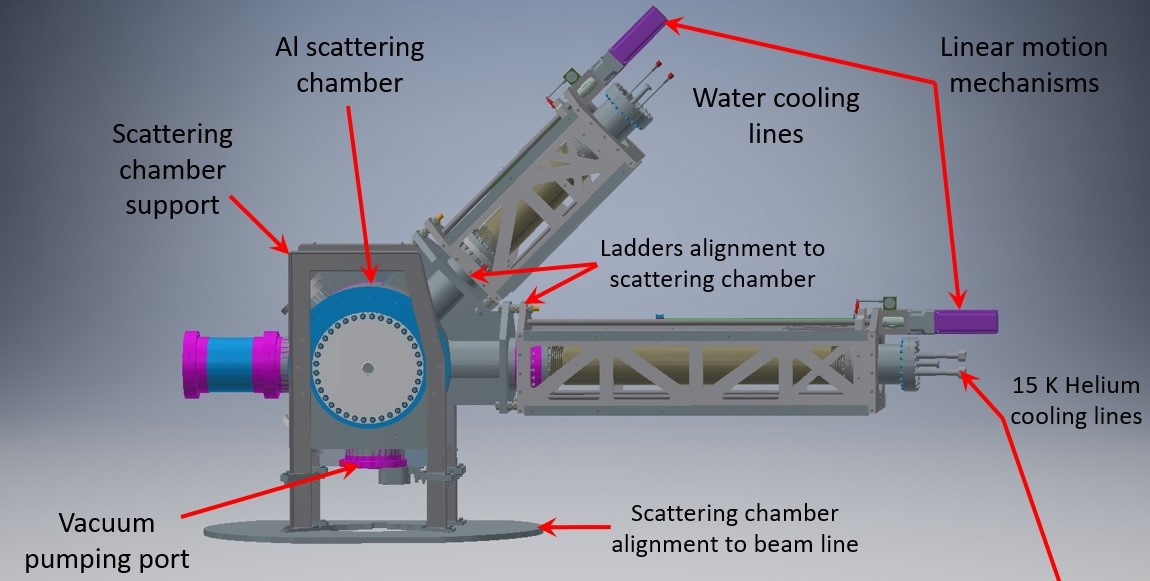
\includegraphics[width=\linewidth]{target_chamber}
    \caption{Scattering chamber of PREX-II/CREX}
    \label{fig:scattering_chamber}
\end{figure}
\begin{figure}[h!]
    \centering
    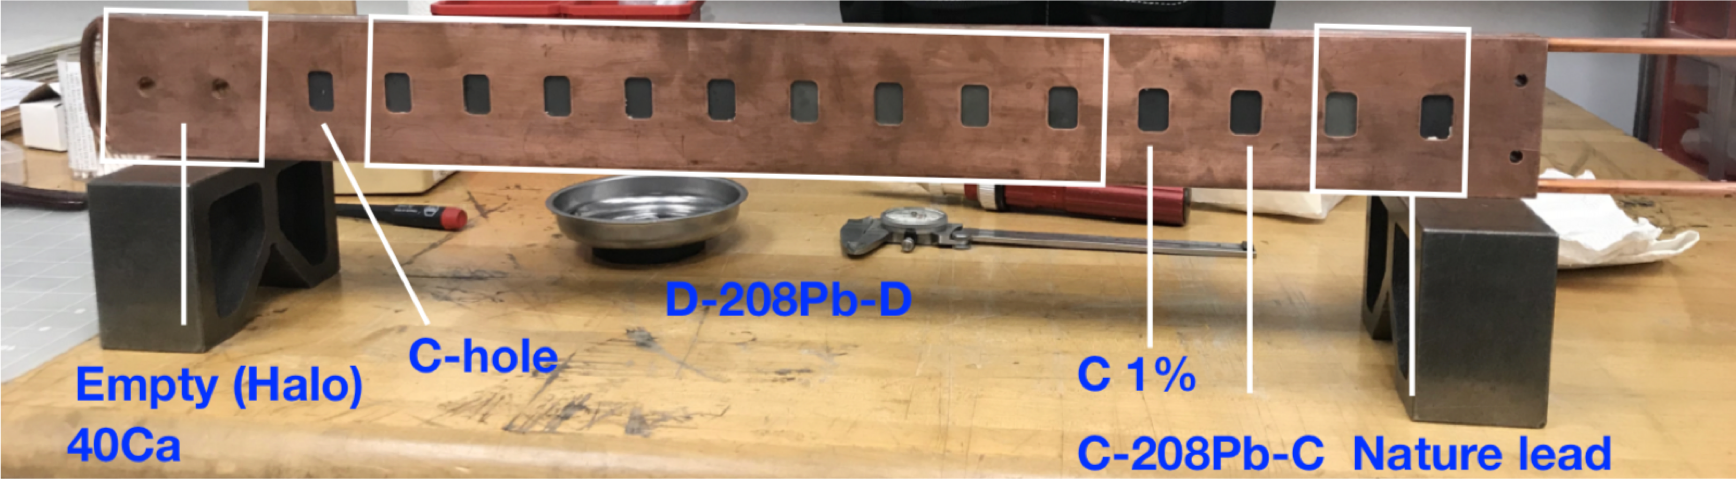
\includegraphics[width=0.6\linewidth]{target_ladder}
    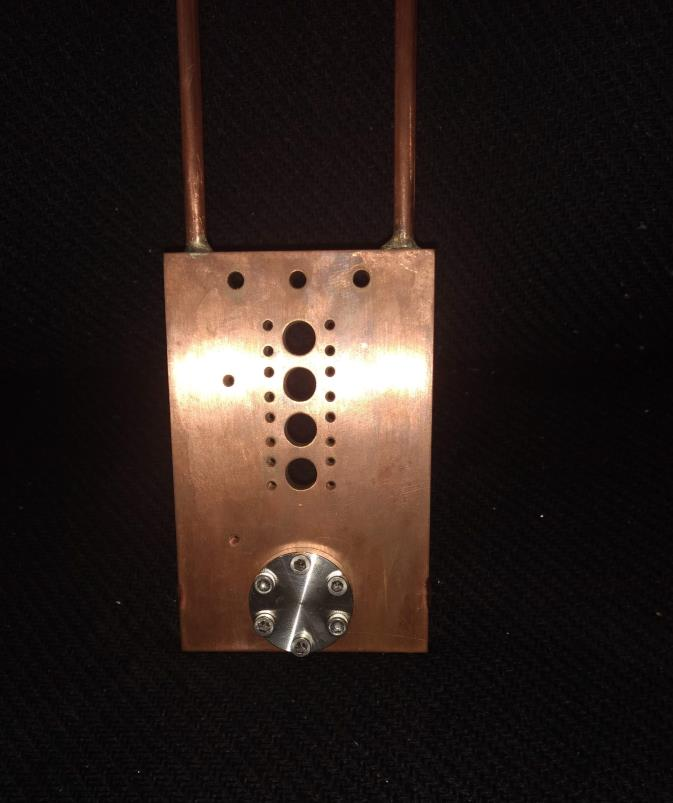
\includegraphics[width=0.25\linewidth, angle=90]{calibration_ladder}
    \caption{Production target ladder and calibration ladder}
    \label{fig:target_ladder}
\end{figure}

The \ca and \Ca targets were installed on the cold heat sink in dedicated cylindrical 
sockets at the end of the production ladder. % tilted $45^\circ$ to beam axis. 
The fact that the \Ca and the \Pb 
targets share the same ladder means they actually had the same z location,
therefore the same scattering angle, to save some effort in the re-installation 
and re-commission of the target chamber.

Special care was needed for \Ca target, the pressure should be less than $10^{-6}\ tort$
to avoid Ca oxidation. The vacuum of the target chamber was maintained by a 
turbo-molecular pumpoing system, which created a $10^{-7}\ (10^{-8})\ torr$ vacuum 
for the calibration (production) ladder in the target chamber. What's more,
gate valves were closed to isolate the target chamber from upstream and downstream
beam pipes when beam was not on. By way of precaution, a nitrogen purge system 
was installed to purge air in case of possible leak.
Every time we warmed up the \Ca target, boiling was needed before restarting data taking.
% Ca oxidation: CaO, $\text{CaCO}_3$, $\text{Ca}_3\text{N}_2$, $\text{Ca(OH)}_2$

%%%%%%%%%%%%%%%%%%%%%%%%%%%%%%%%%%%%%%%%%%%%%%%%
\subsection{Target Cooling}
The production ladder was cryogenically cooled due to high power from electron beam,
while the calibration ladder was water cooled, the calibration runs need only
$\lesssim 1\ \mu A$ level beam current. Both ladders were made of cooper,
the cooper frame of the production ladder was cooled by $15\ K$, $12\ atm$ gaseous helium, 
which runs through the cooling tube surrounding the frame.
% https://prex.jlab.org/DocDB/0000/000012/001/tgtchamber_err2_17may2017.pdf
For D-Pb-D sandwich target with thick C foil, the heat loading will be $100\ W@70\ \mu A$
with a $4\times 6 \ mm$ raster, the cooling system kept the Pb target stay at
$\ K$ (FIXME) (melting point at $600 \ K$). For \Ca target, With $150\ \mu A$ beam current, 
it will produce about $370\ Watts$ heat on the target, which raised the target temperature to
% TargetOperation.pdf
$\ K$ (FIXEM) (melting point at $1115\ K$).
The max temperature of Ca will reach $203\ K$, assuming perfect contact between
Ca foil and the cooper frame and a $15\ K$ coolant.



%%%%%%%%%%%%%%%%%%%%%%%%%%%%%%%%%%%%%%%%%%%%%%%%
\subsection{Raster}
Although the target foil was cooled to about $20\ K$ (PREX-II), it still deformed (even melted)
under electron's bombardment. Small nonuniformities in the target 
thickness vary the scattering rate, and over the course of the experiment they 
eventually generated enough noise to swamp the tiny weak-scattering signal.
Actually, this is how we inspect the status of a target and evidence to
replace a target if the measured asymmetry width increase significantly.

\begin{figure}
    \centering
    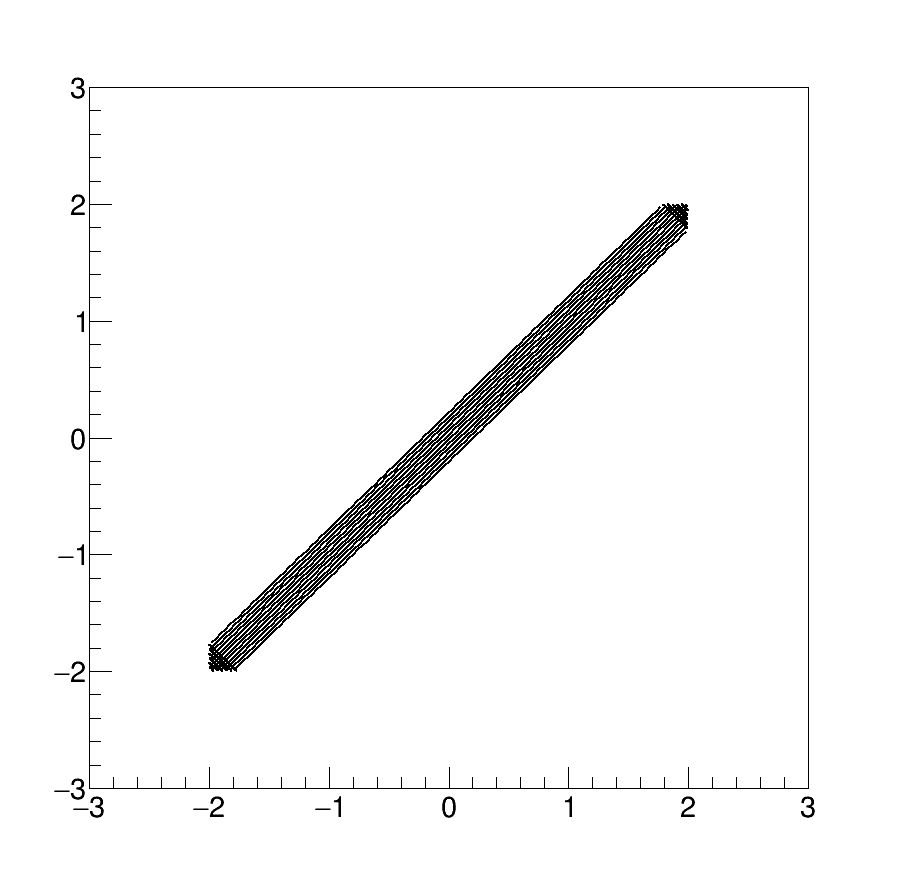
\includegraphics[width=0.48\linewidth]{raster_pattern_1}
    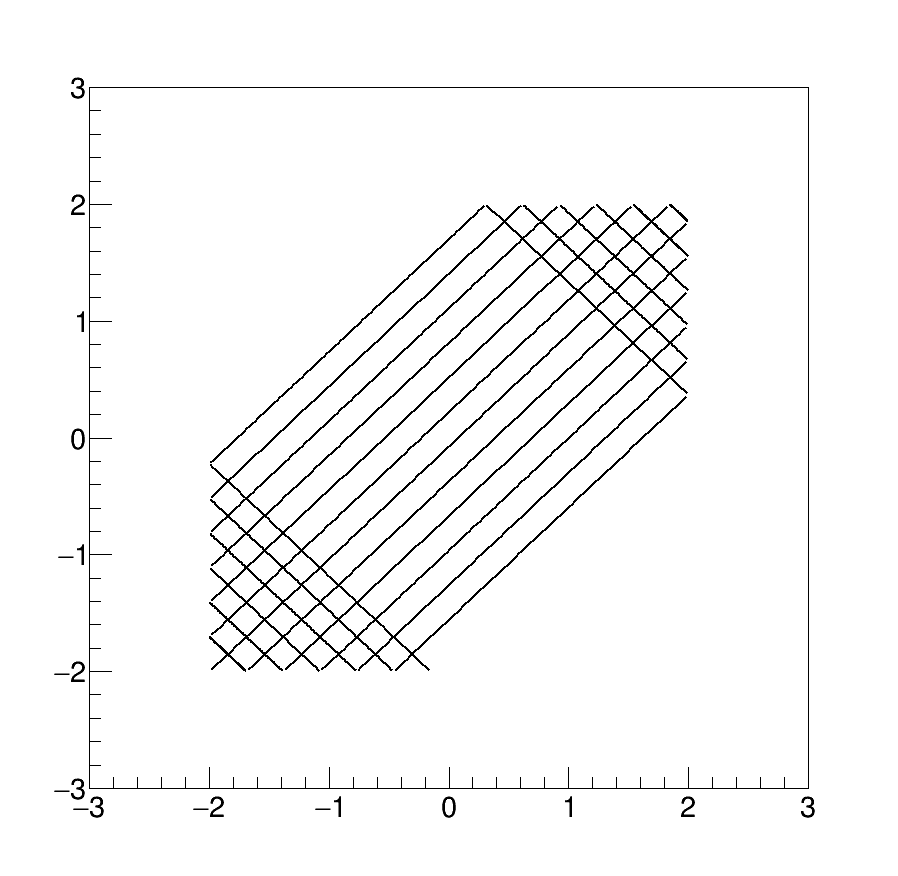
\includegraphics[width=0.48\linewidth]{raster_pattern_2}
    \caption{Raster pattern with different frequency difference between X and Y.
    Left: $|f_y - f_x| = 120\ Hz$; Right: $|f_y - f_x| = 8*120\ Hz$. The raster
    shape is a $4\times 4\ mm$ square.} 
    \label{fig:raster_pattern}
\end{figure}

The solution to this problem is the raster, which is a set of dipole magnets % where are they
that deflect the beam at about $25\ kHz$ to spread the beam on the target.
What we learned from PREX-I was that we could significantly reduce the sensitivity 
to target-thickness variations by synchronizing the helicity flipping frequency
with the raster frequency so that it sampled different areas on the target. 
As shown in Fig. \ref{fig:raster_pattern}, the Lissajous pattern we got depends
on the frequency difference between X and Y, the larger the frequency difference,
the larger the scanning area. The ratio of $f_y/f_x$ should be an irrational number
to prevent a closed Lissajous pattern. The actual freqeuncies we used were $25.44$
and $24.48\ kHz$, for PREX-II, the raster size was $4 \times 6\ mm$, and CREX
had a raster size of $2 \times 2\ mm$.
% https://prex.jlab.org/wiki/index.php/Raster_Scope

\begin{figure}
    \begin{tikzpicture}
	\begin{scope}
	    \node[anchor=south west, inner sep=0] (image) at (0, 0)
	    { 
	    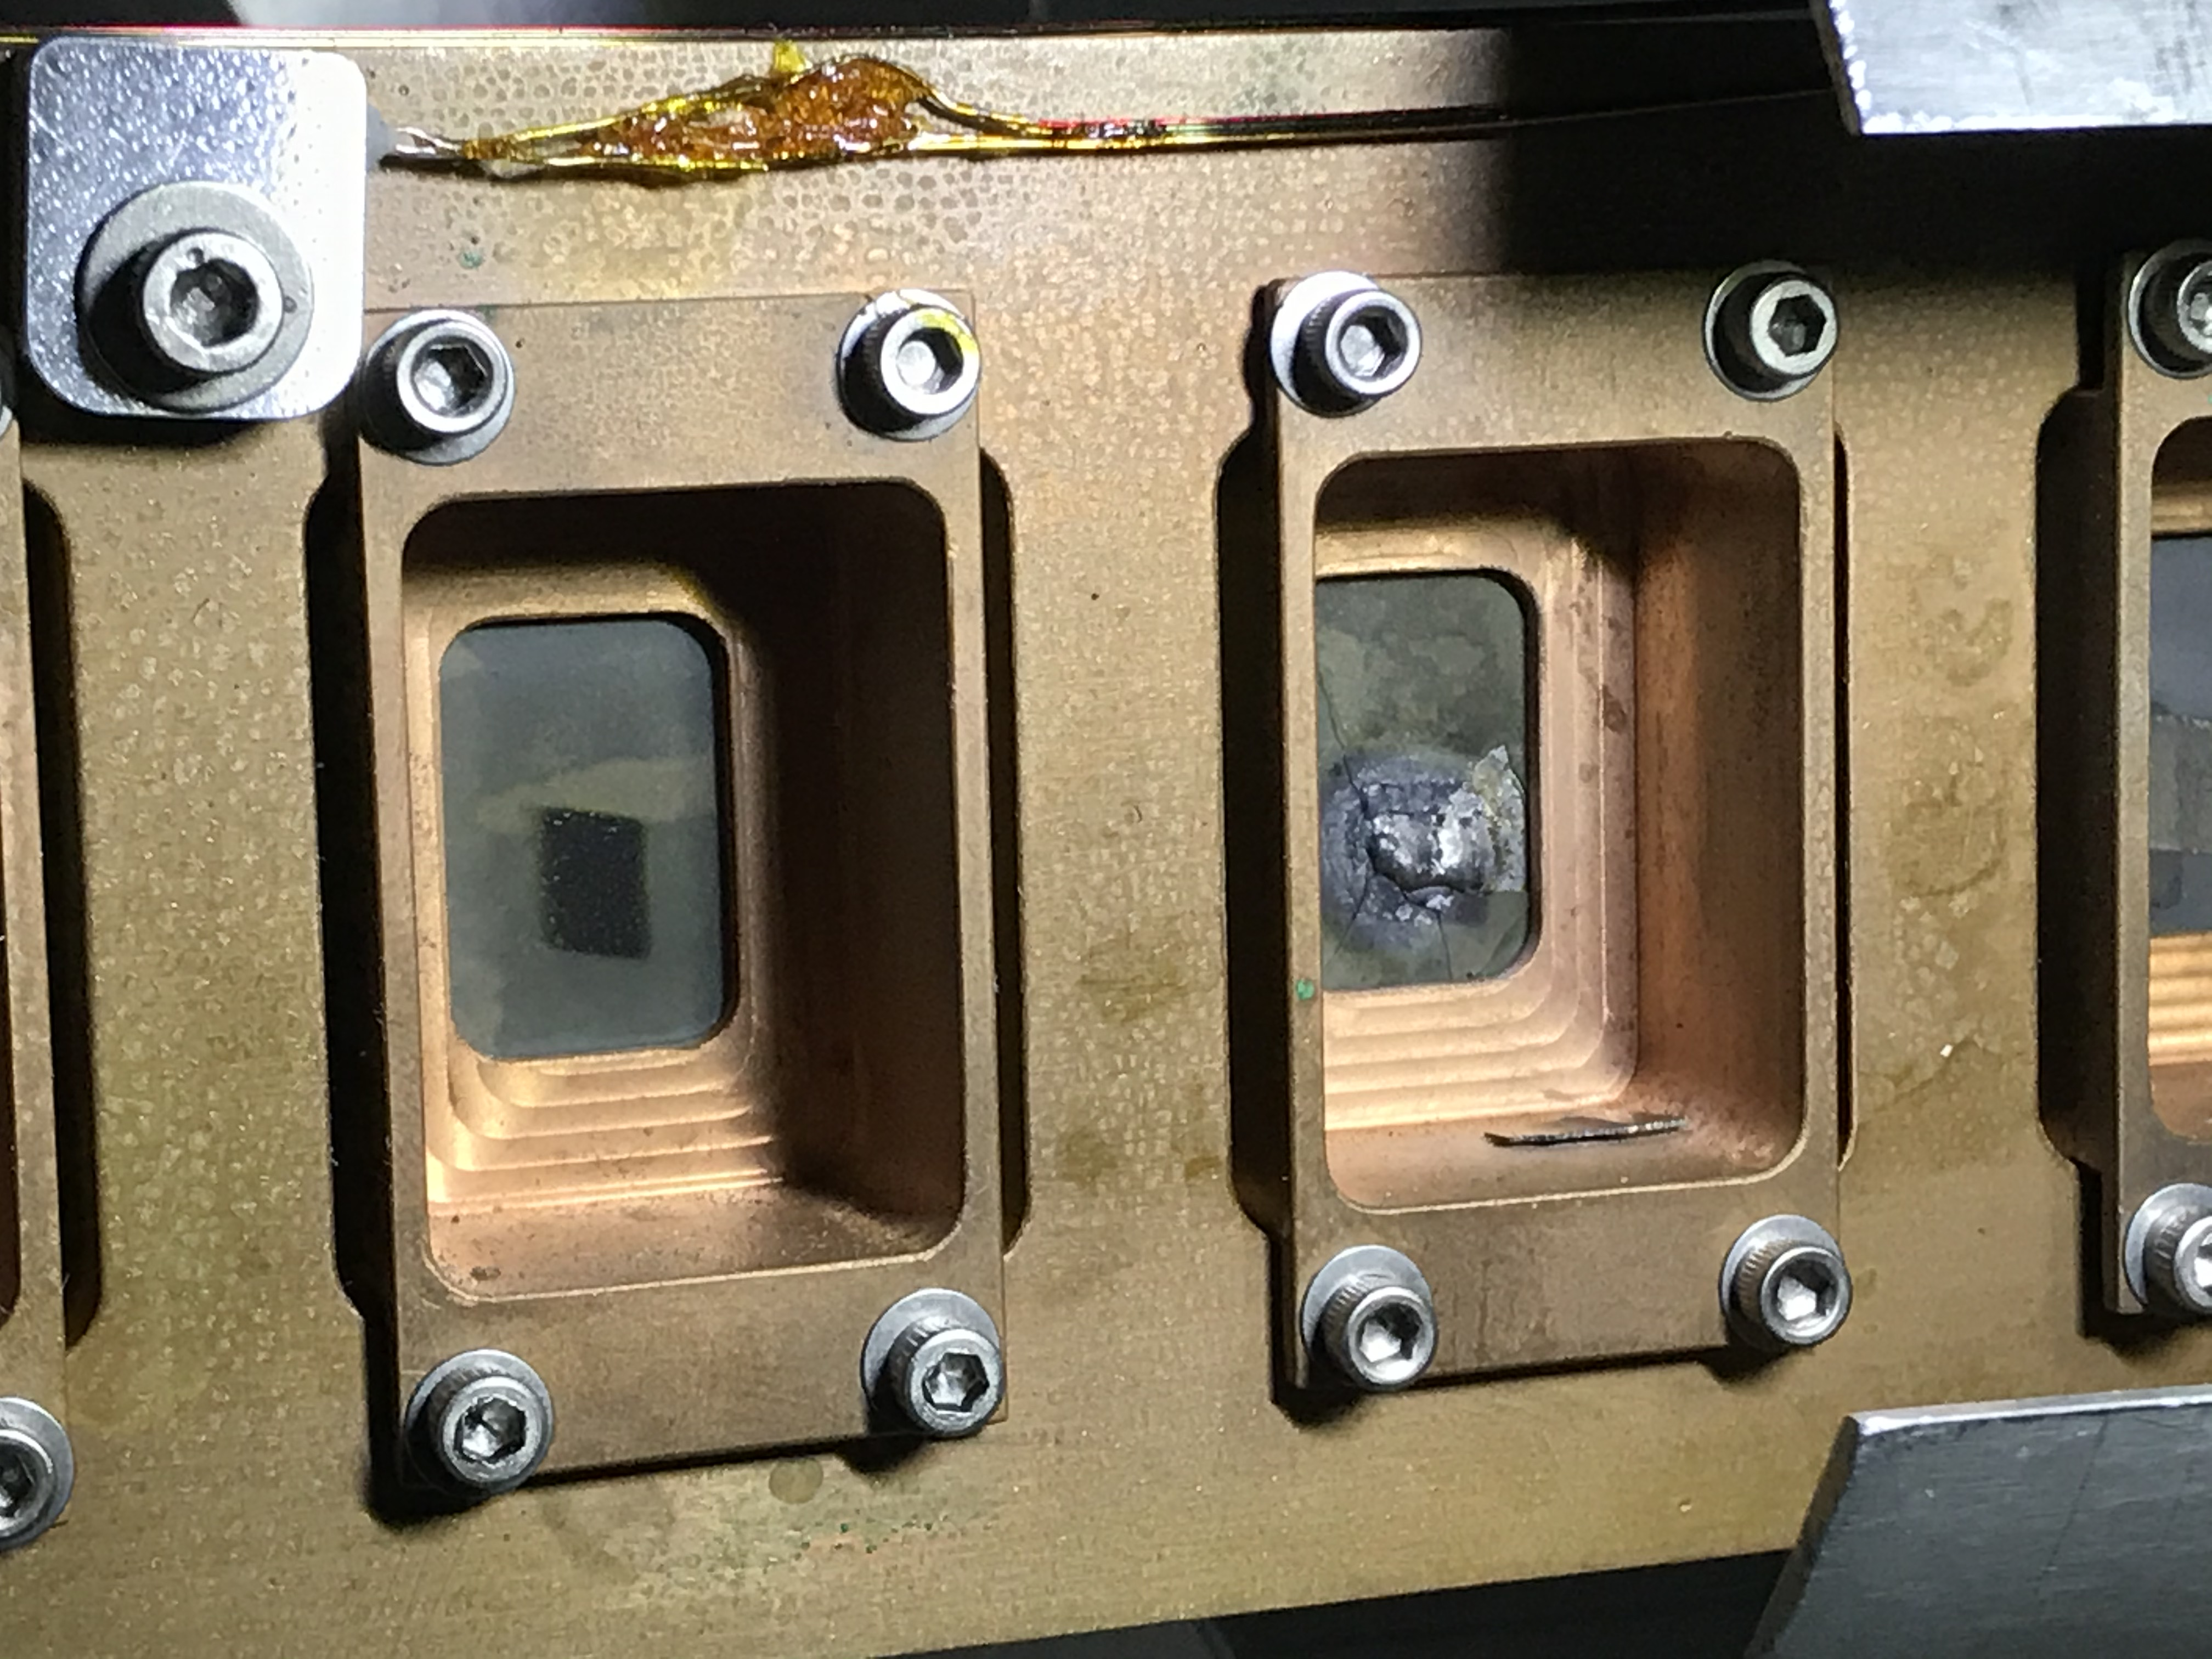
\includegraphics[width=0.32\linewidth]{prex_post_target_1}
	    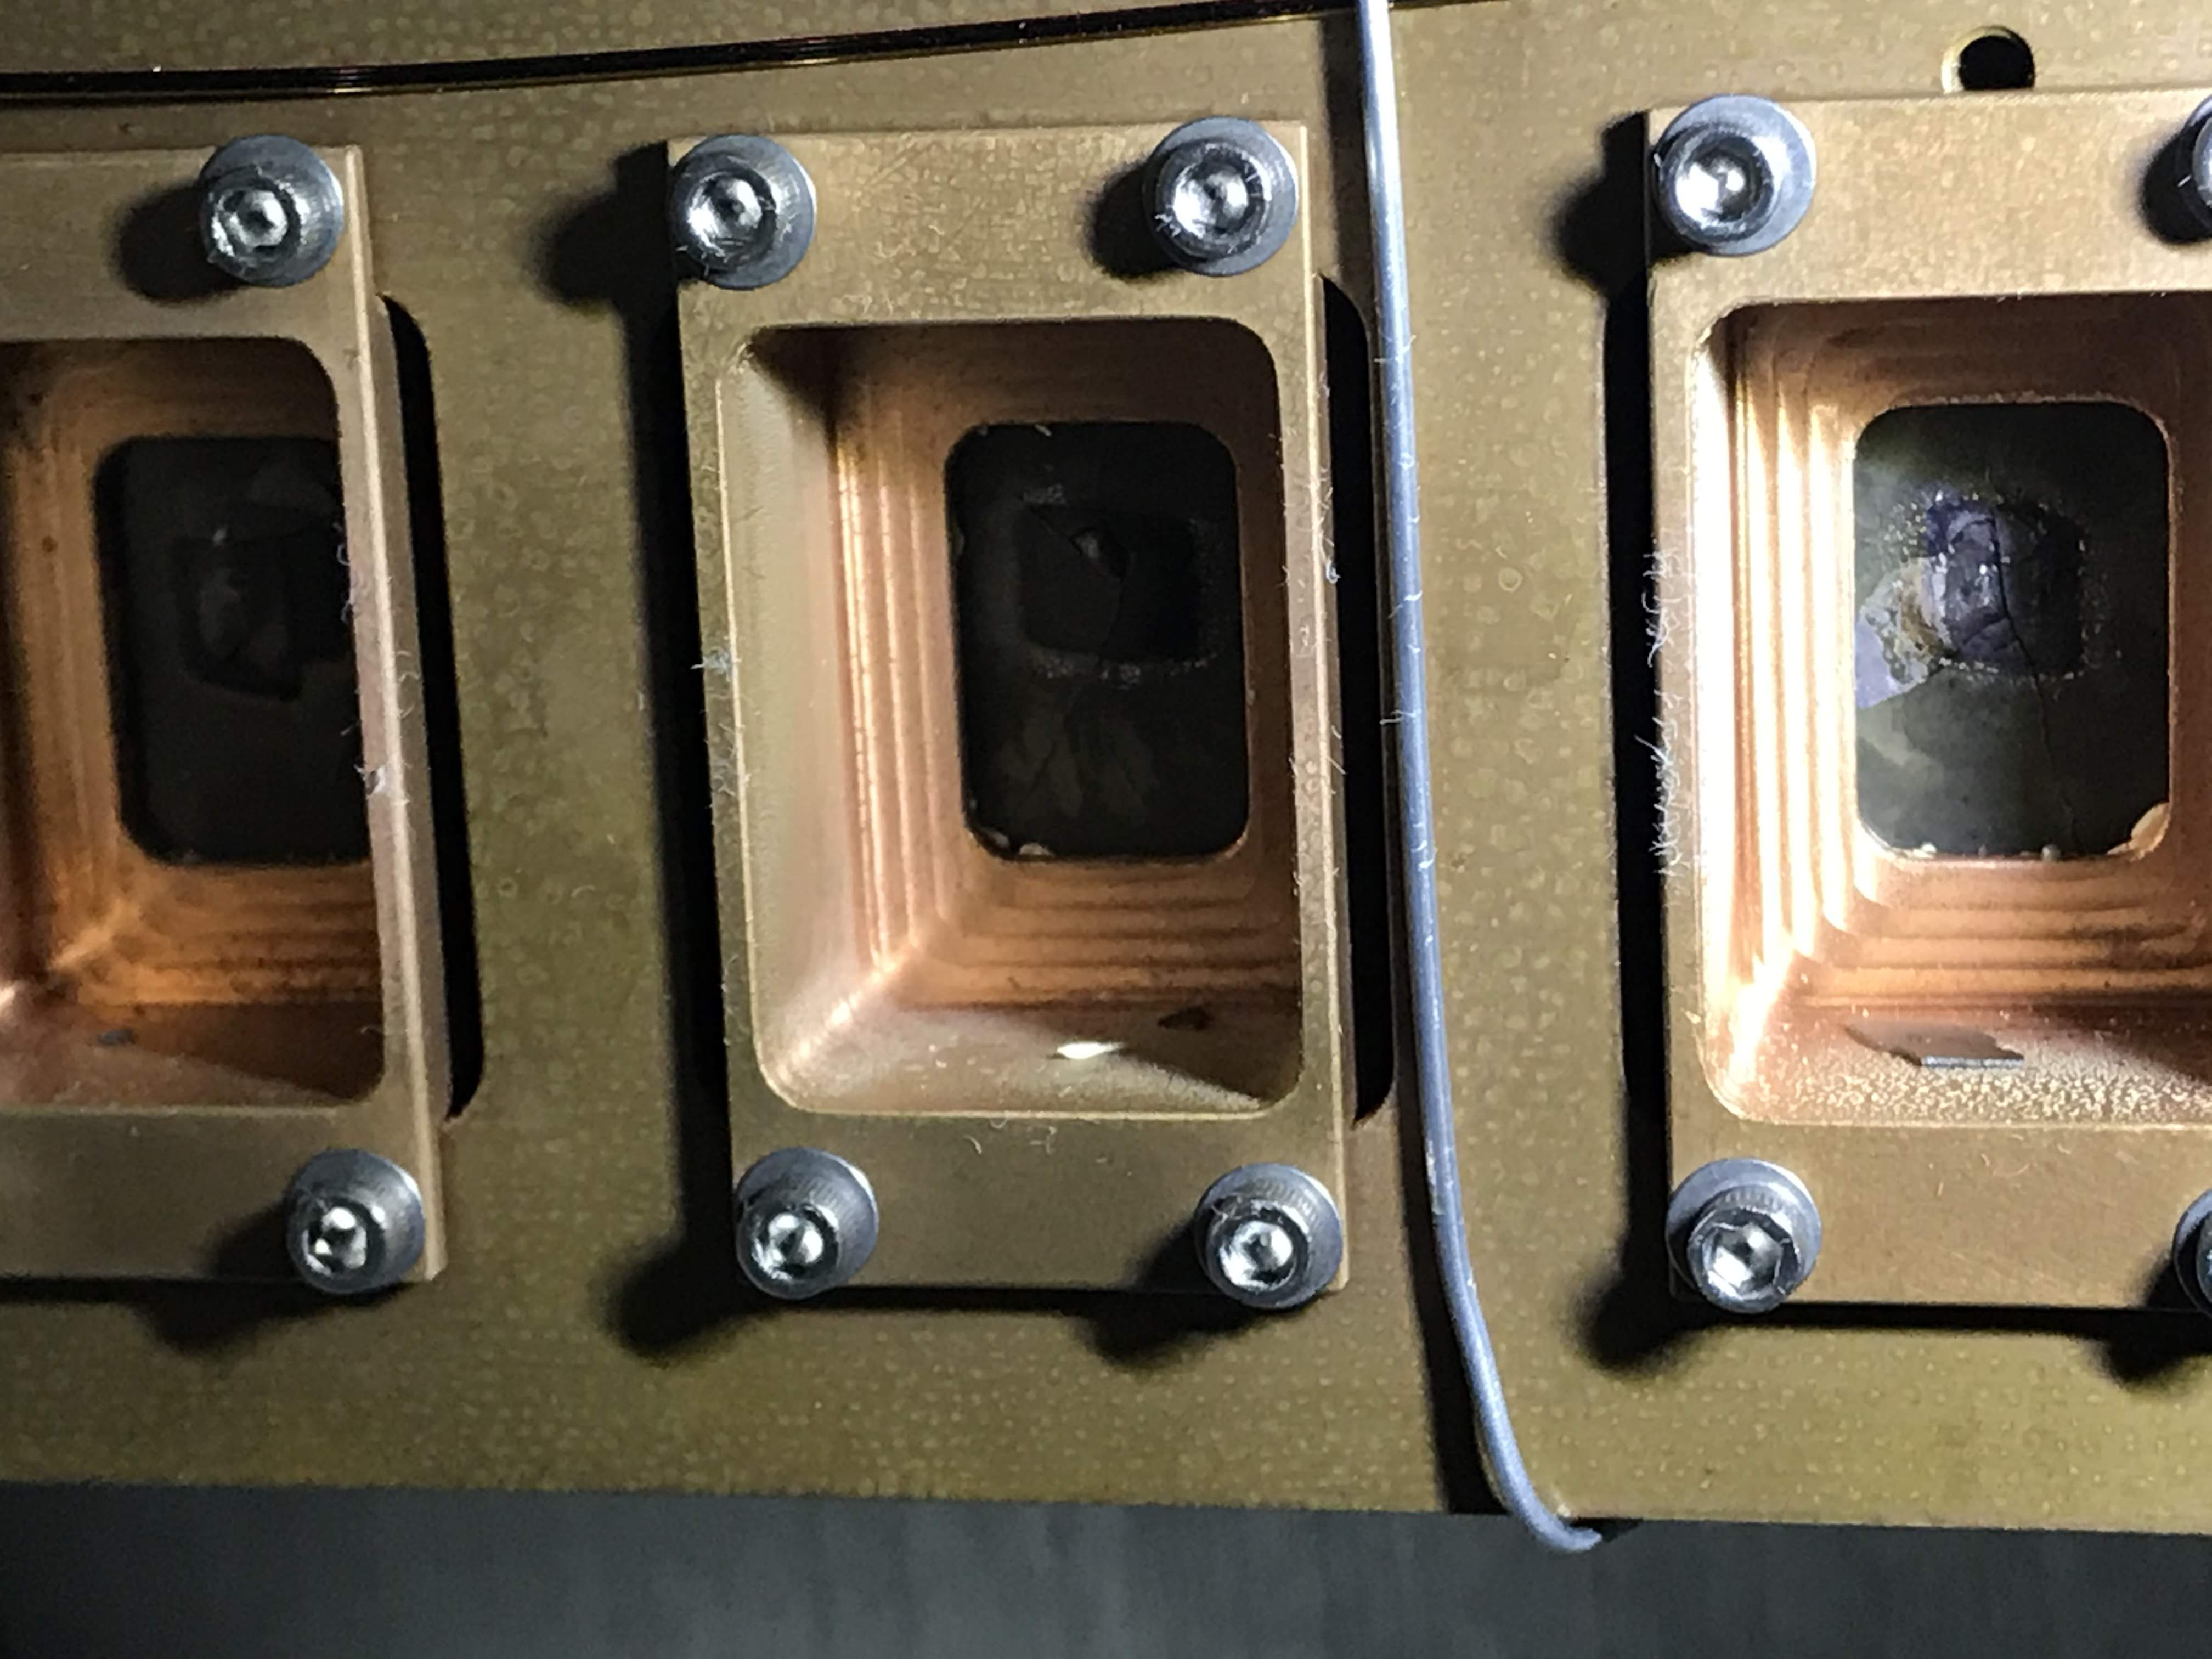
\includegraphics[width=0.32\linewidth]{prex_post_target_4}
	    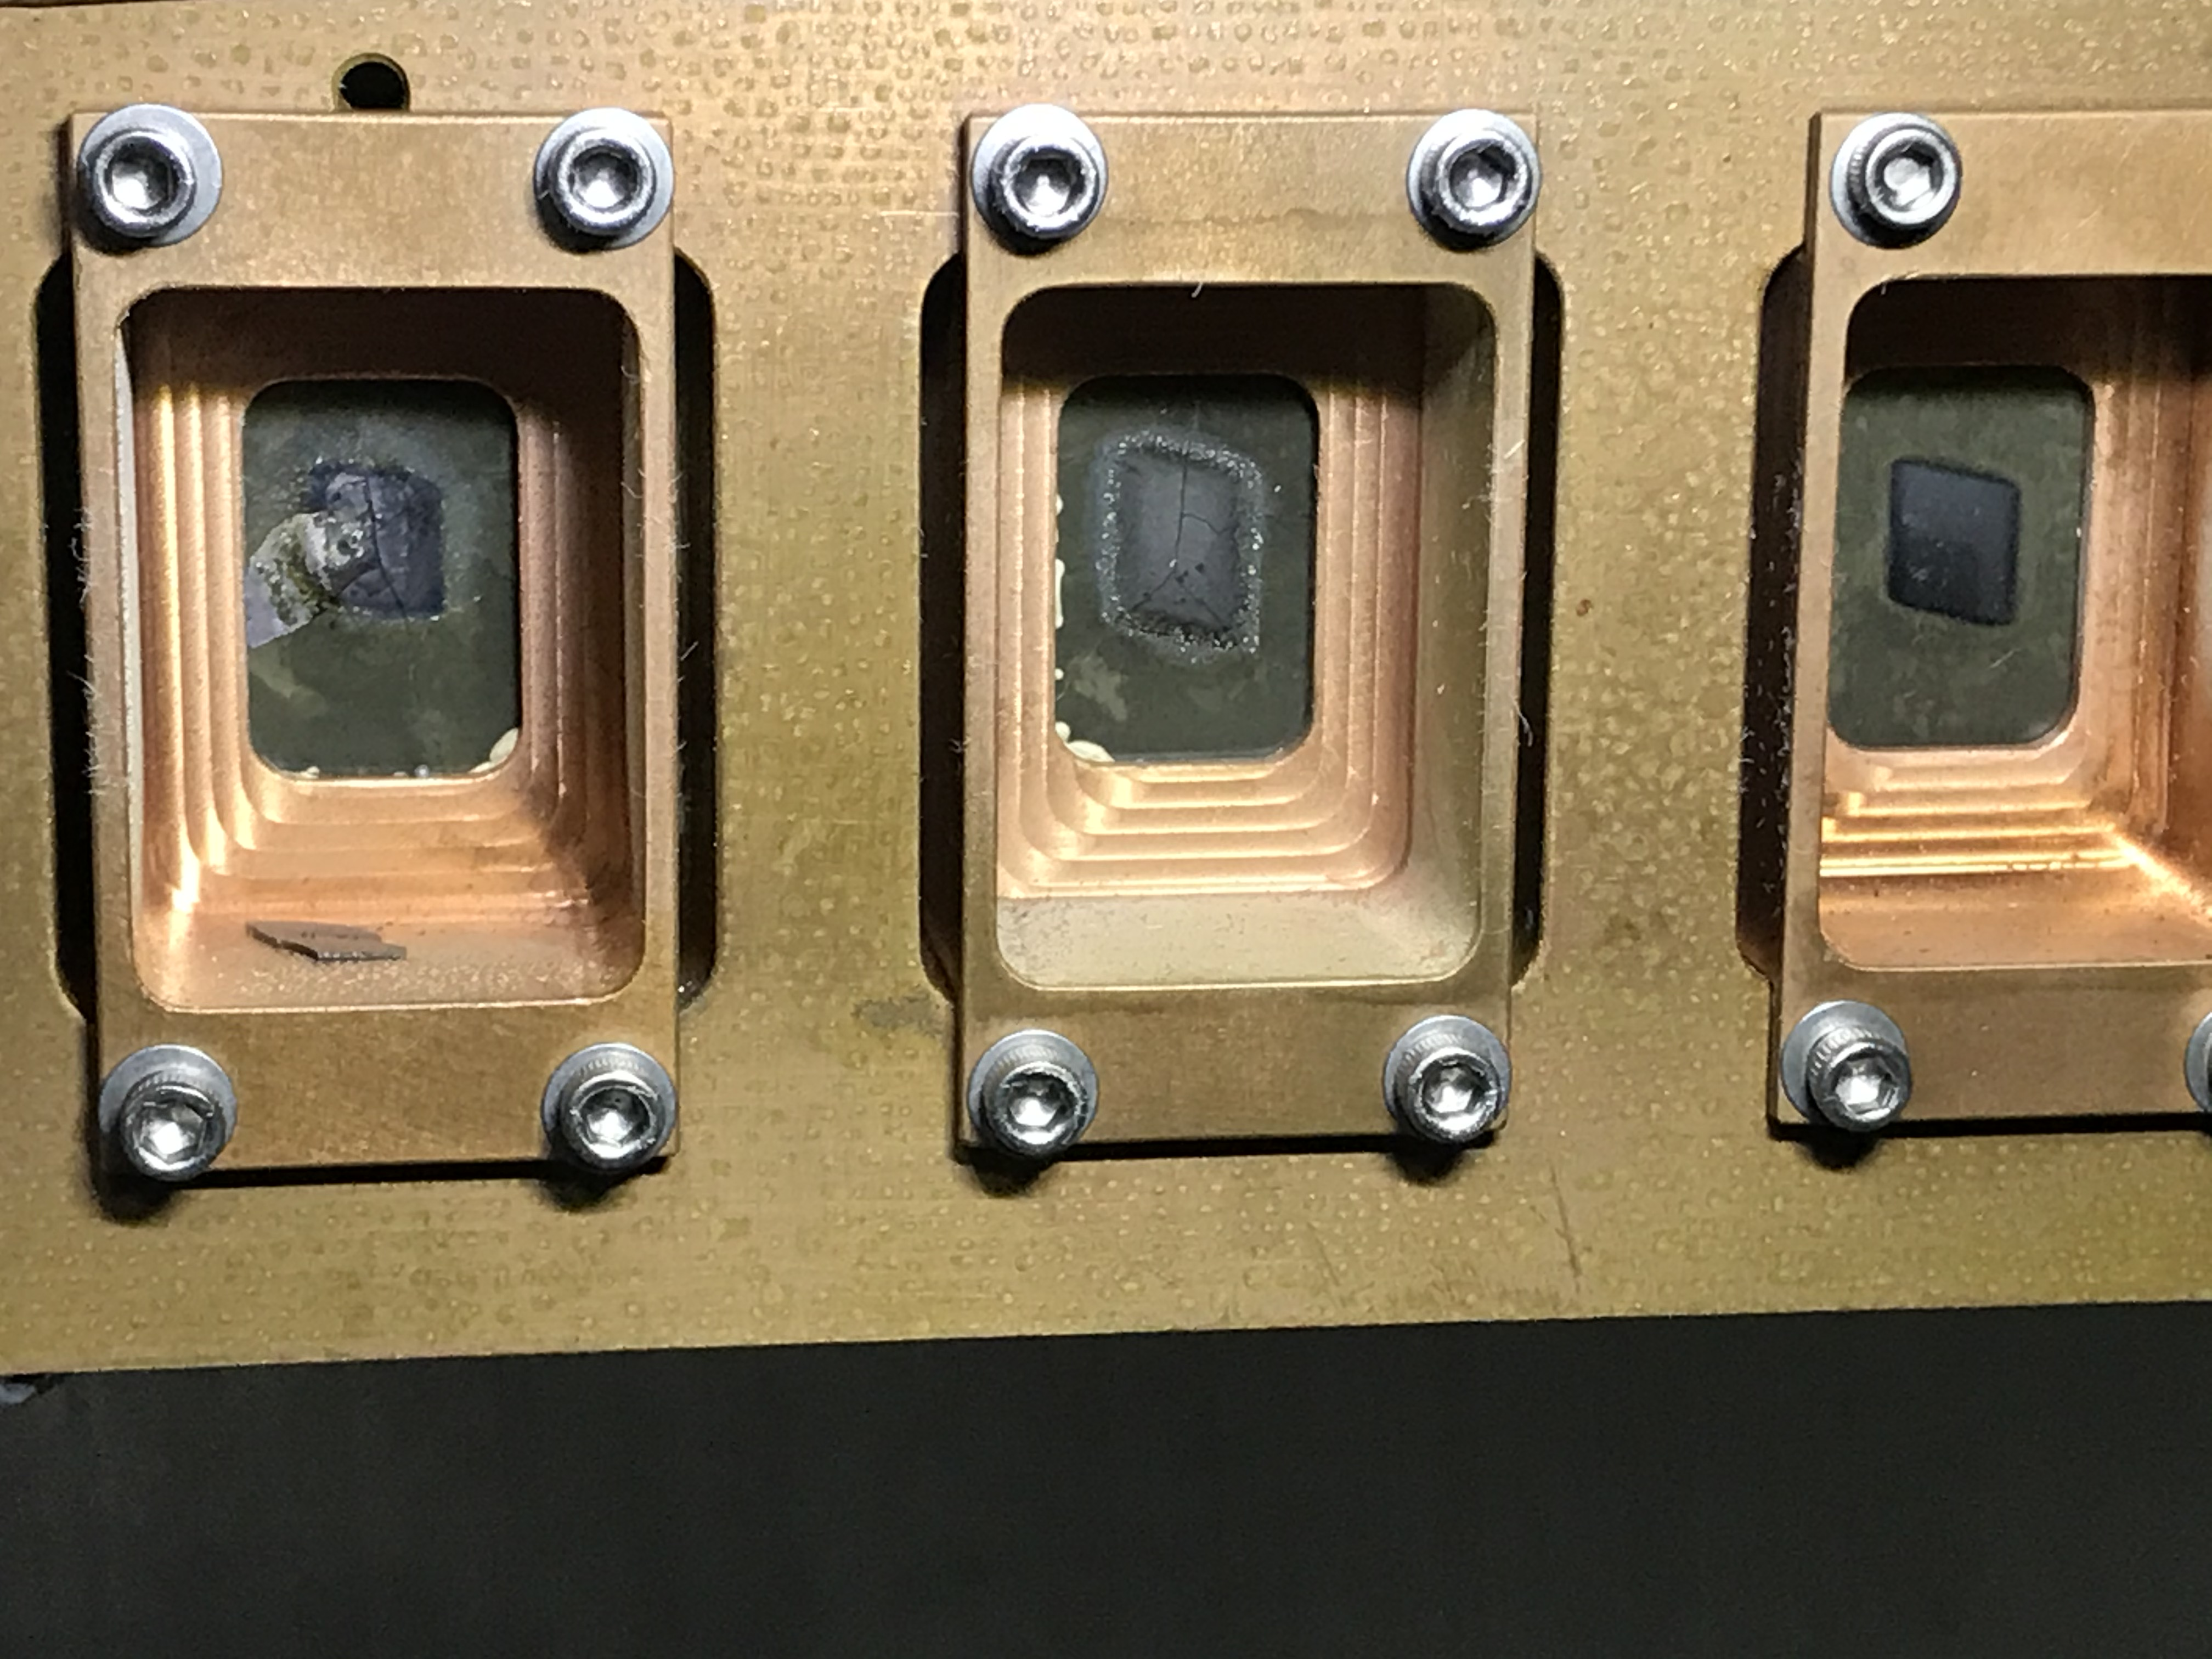
\includegraphics[width=0.32\linewidth]{prex_post_target_3}
	    };
	    \begin{scope}[x={(image.south east)}, y={(image.north west)}]
		\node [red] at (0.105, 0.19) {\textbf{Unused}};
		\node [red] at (0.235, 0.19) {\textbf{1}};
		\node [red] at (0.355, 0.22) {\textbf{2}};
		\node [red] at (0.49, 0.22) {\textbf{3}};
		\node [red] at (0.63, 0.22) {\textbf{4}};
		\node [red] at (0.73, 0.28) {\textbf{4}};
		\node [red] at (0.855, 0.28) {\textbf{6}};
		\node [red] at (0.975, 0.28) {\textbf{7}};
	    \end{scope}
	\end{scope}
    \end{tikzpicture}
    \caption{Picture of Pb targets after running, one can see clearly the shape
    of raster.}
\end{figure}

Another reason for having raster is heat dissipation, the larger the raster size,
the quicker the heat dissipation will be, the lower the target temperature, as
shown in Fig. \ref{fig:target_temp_with_raster}.
\begin{figure}
    \centering
    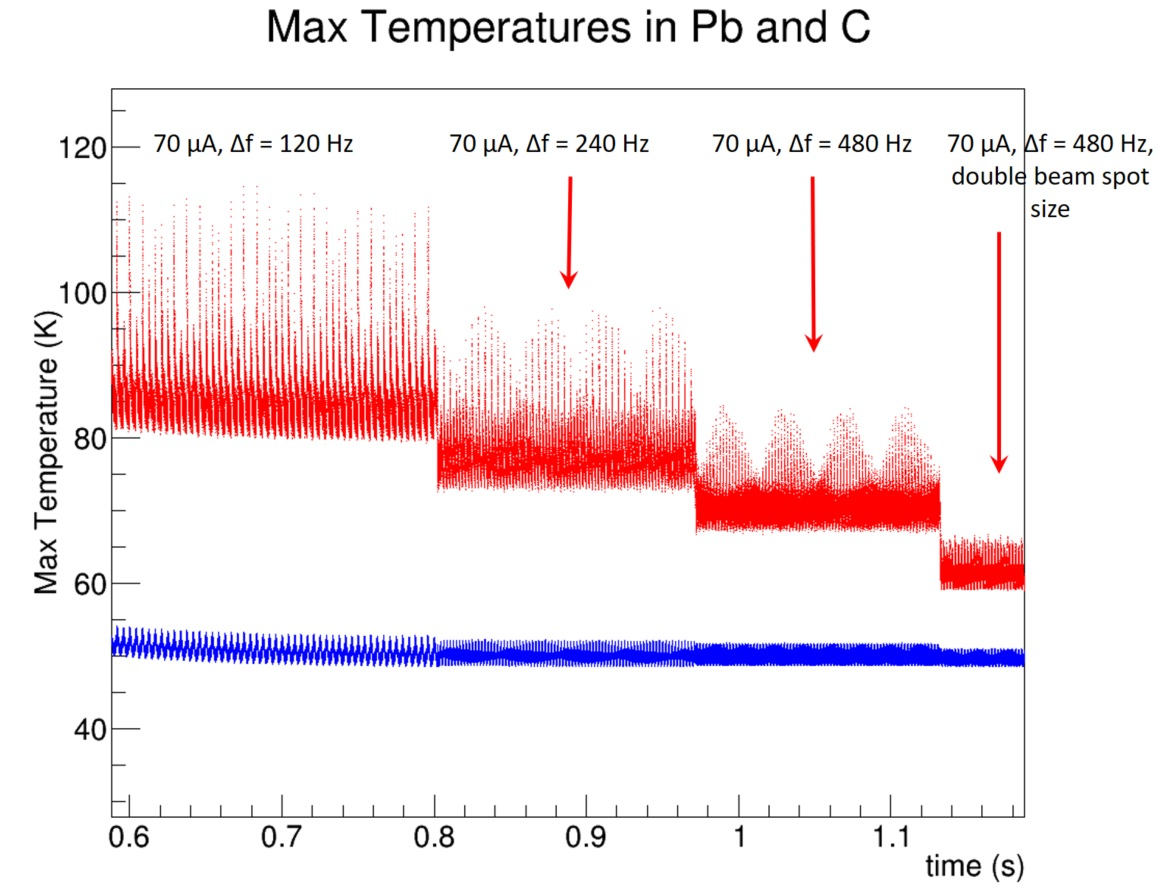
\includegraphics[width=0.5\linewidth]{target_temp_with_raster}
    \caption{How the target temperature change with size of raster area.}
    \label{fig:target_temp_with_raster}
\end{figure}

%%%%%%%%%%%%%%%%%%%%%%%%%%%%%%%%%%%%%%%%%%%%%%%%
\subsection{Beamline Collimator}
\begin{figure}[h!]
    \centering
    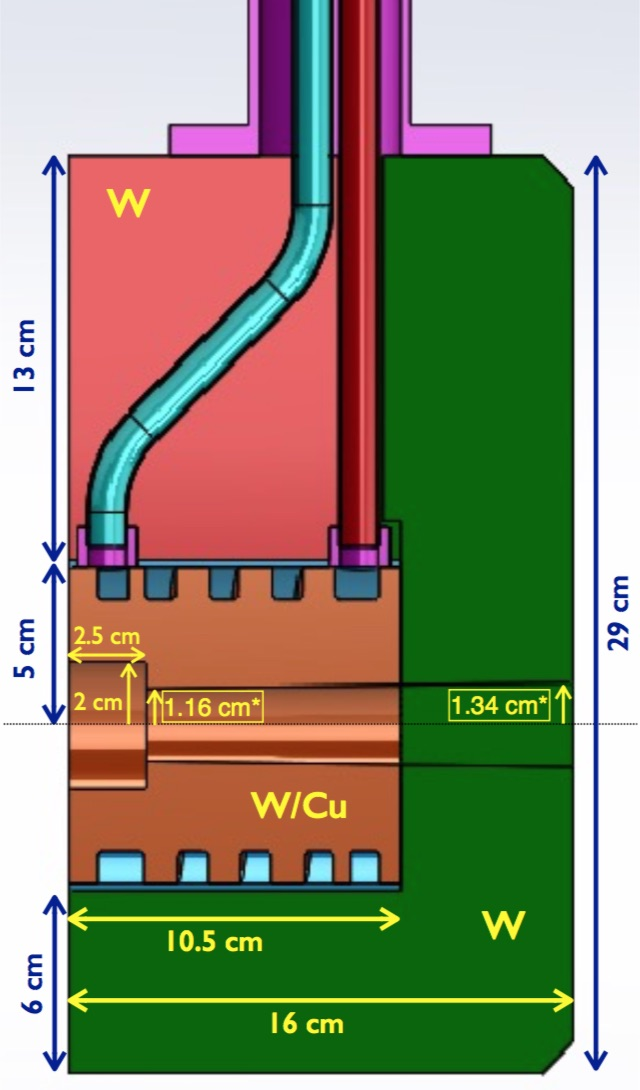
\includegraphics[height=0.23\paperheight]{beamline_collimator_side}
    \hspace{1 cm}
    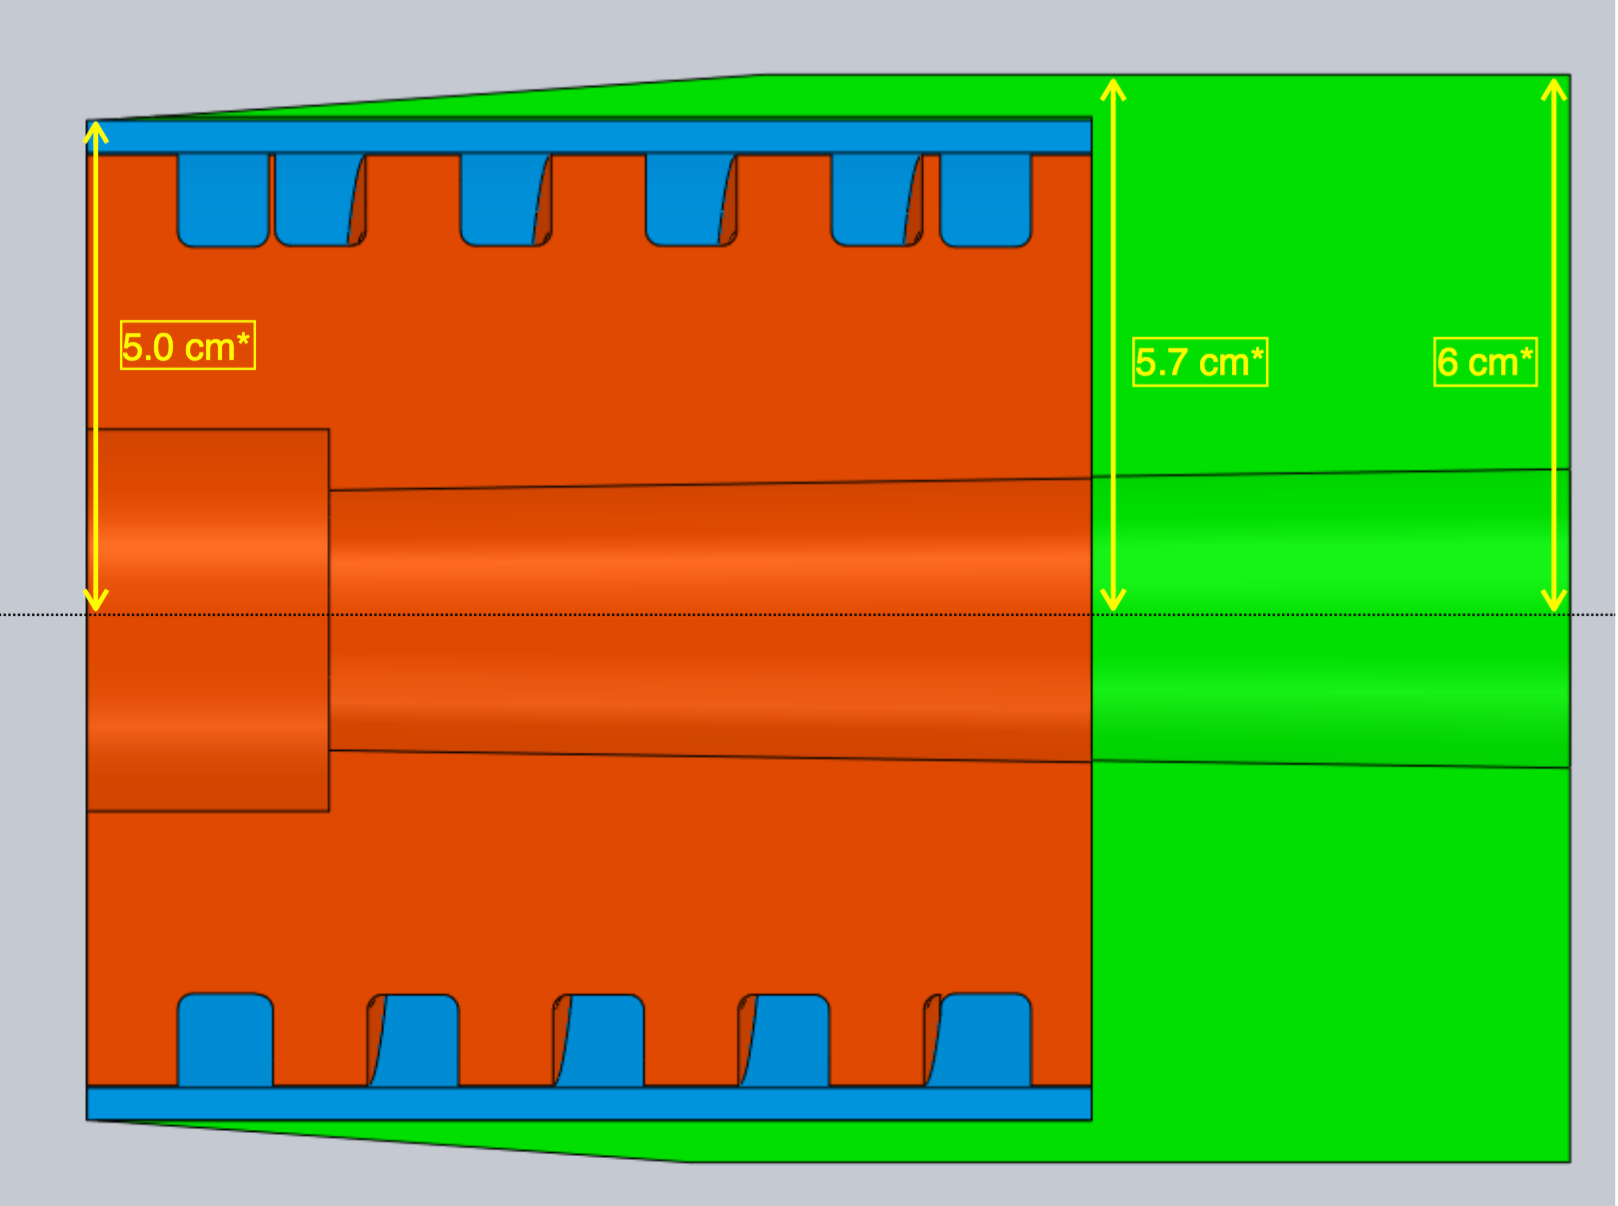
\includegraphics[width=0.4\linewidth]{beamline_collimator_top}
    \caption{Side and top view of beamline collimator. Beam from left to right.}
    \label{fig:beamline_collimator}
\end{figure}

Another problem that failed PREX-I was the excessive radiation, which damaged 
electronics in the Hall and the o-ring on the target exit flange leading to
leaks and ultimately halted the experiment.
% https://mailman.jlab.org/pipermail/halla_parity/2010-April/000197.html
With this experience, the new design of the pivot area (the center of the 2 HRS 
where the target chamber lies in) for PREX-II and CREX payed more attention
to radiation near the target region. The idea was to lead as much radiation to
beam dump as possible, and absorb the rest radiation in one key component --
the beamline collimator, which was placed $83\ cm$ downstream of the production 
target. The beamline collimator consists of an inner collimator and a housing
jacket made of sintered tunsgsten; the inner collimator, in turn, has the same 
structure of a 70\% W/30\% Cu alloy collimator and a copper jacket. As shown
in Fig. \ref{fig:beamline_collimator}, there is cylinder notch in the front of
the inner collimator, to make sure the electrons/radiation are completely 
absorbed inside the collimator. The beamline collimator was water cooled, with
maximum heat loading of about $3.65\ kW$ from Pb target. The power on the beamline
% ffrom my simulation note
collimator was another signal for the degration of target. When the temperature 
of the outgoing water increased dramatically, it was time to replace the target.
as shown in Fig. \ref{fig:collimator_see_target_degration}

Besides the beamline collimator, a few other devices were installed 
to further eliminate the radiation level in the hall. These devices include the 
high-density polyethylene (HDPE) neutron shield around the beamline collimator
region and a skyshine shield consisting of a $6\ cm$ thick tungsten block and
massive concrete blocks. These extra shields were used to block high energy
neutrons from the collimator.

\begin{figure}[h!]
    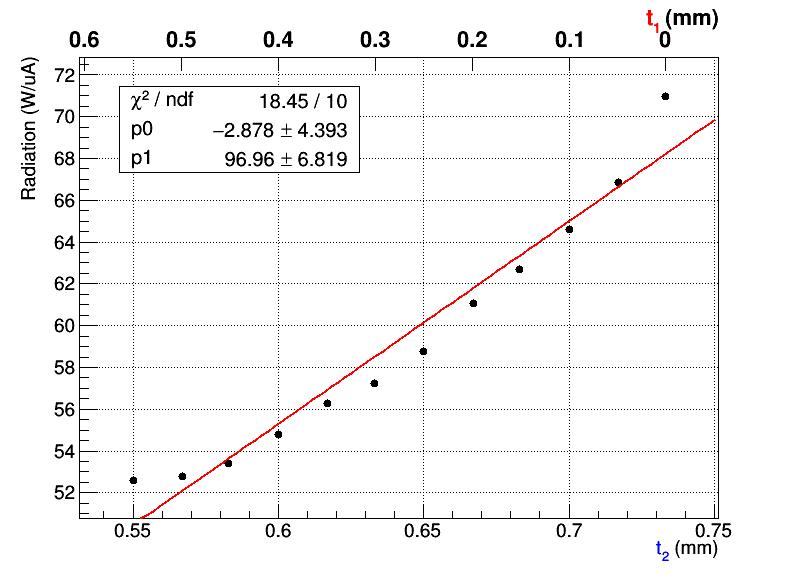
\includegraphics[width=0.32\linewidth]{collimator_power_fit}
    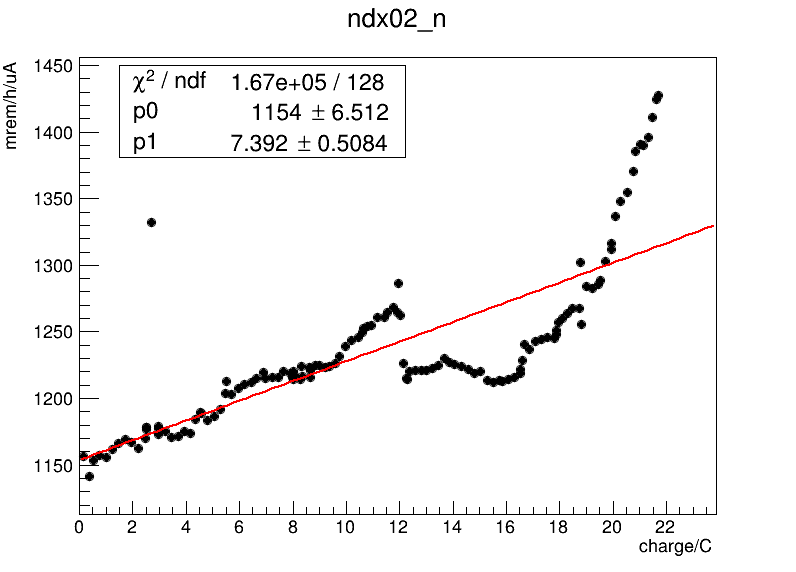
\includegraphics[width=0.32\linewidth]{Pb10_ndx02_n}
    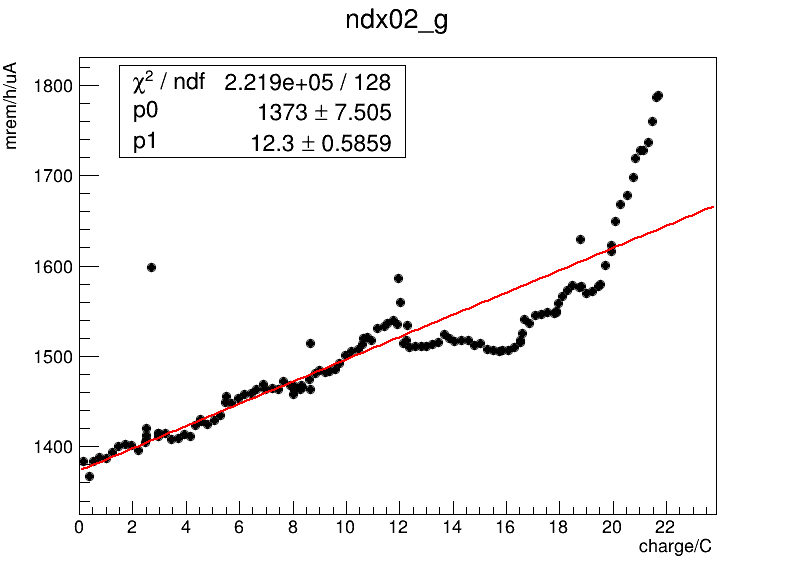
\includegraphics[width=0.32\linewidth]{Pb10_ndx02_g}
    \caption{Left: a simple model of target degration -- assumming the inner 
    foil ($t_1$) is becoming thinner and the outer foil is becoming thicker ($t_2$) 
    while the total mass keeps intact. The plot showes how the power deposition 
    on the beamline collimator change in this model. Middle and Right: actual
    neutron and photon radiation level monitored along charge accumulation. They
    show similar trends.}
    \label{fig:collimator_see_target_degration}
\end{figure}
% PREX-I O-ring failure: a large raster and a high current: 
% https://hallaweb.jlab.org/halog/html/1004_archive/100413092229.html


%%%%%%%%%%%%%%%%%%%%%%%%%%%%%%%%%%%%%%%%%%%%%%%%
\subsection{Septum}
The septum magnet is required to bridge the scattered electrons at small angle
into the HRS. As said before, the designed scattering angle is about $5^\circ$
while the smallest angle that HRS can reach is $12.5^\circ$, so we need the septum
magnet to guide the scattered electrons into HRS. 

The septum magnets are normal conducting magnets that consist of 3 coils, 
by applying large current, it will produce a
strong magnetic field (up to $\sim 1 \ T$ in the central region). A septum beampipe
will connect the upstream collimator box and the downstream HRS vacuum pipe.

\begin{figure}[h!]
    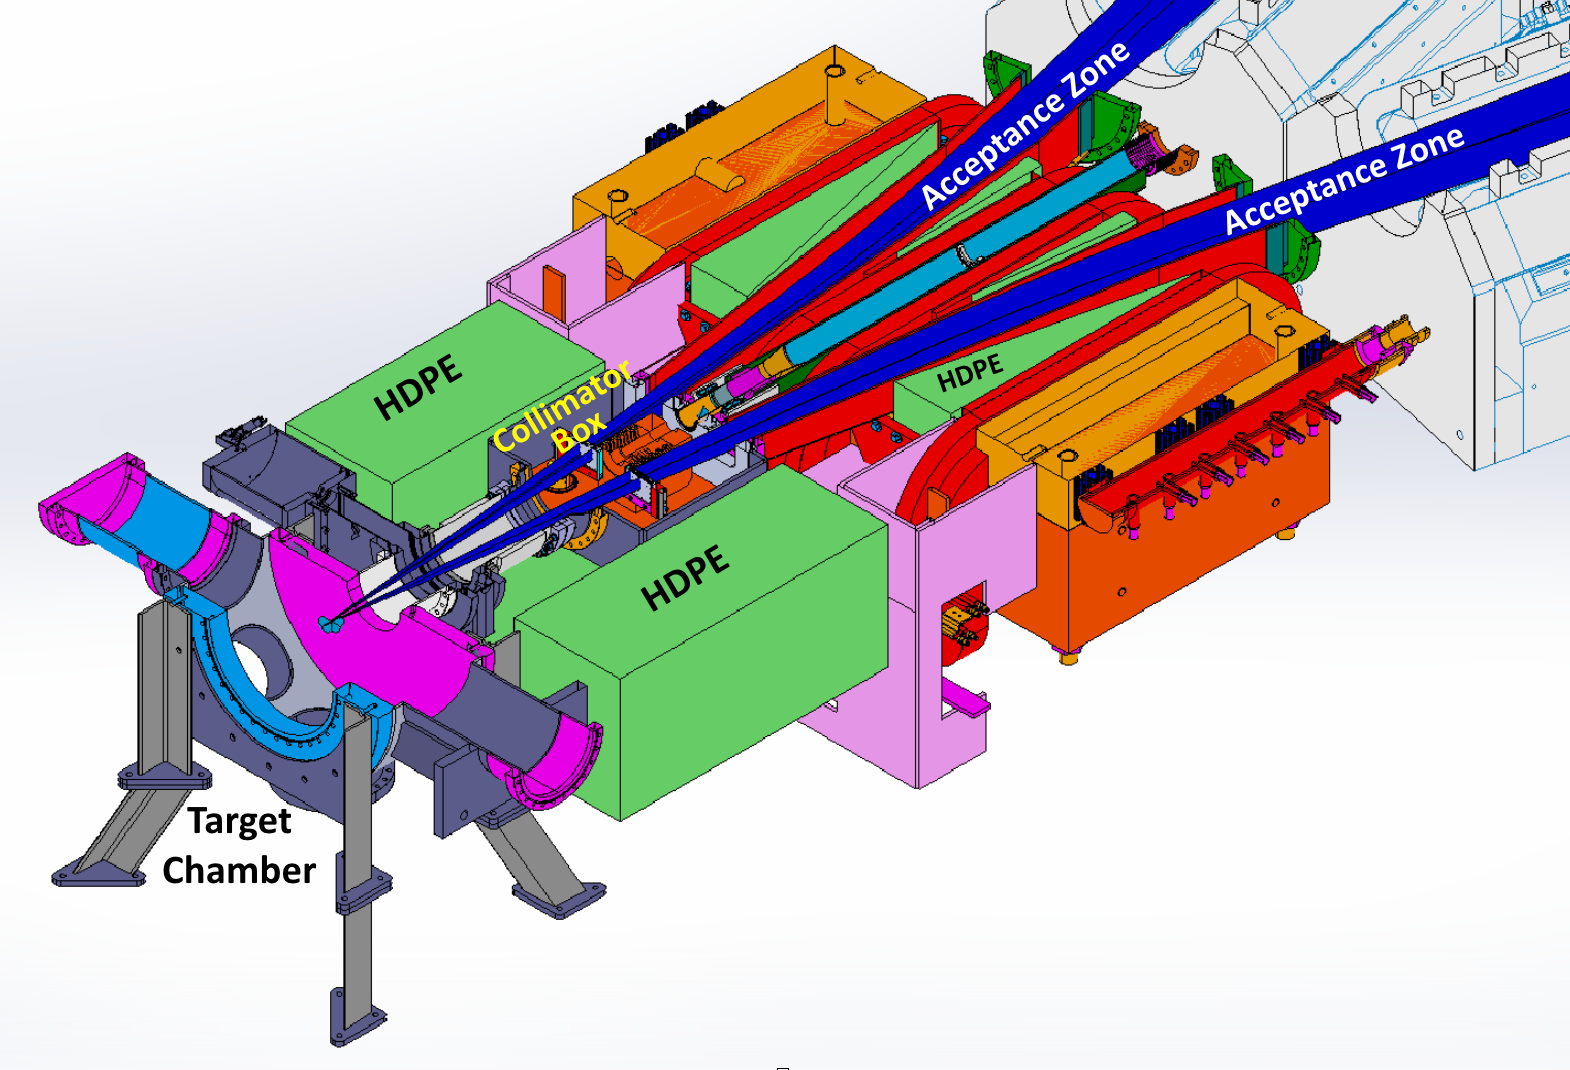
\includegraphics[width=0.52\linewidth]{septum}
    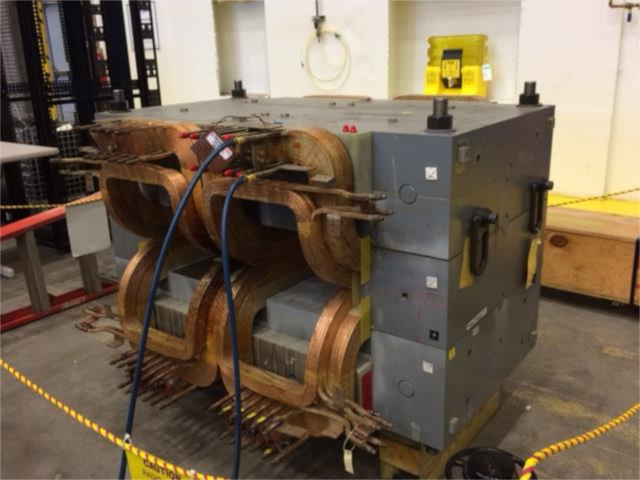
\includegraphics[width=0.46\linewidth]{septum_real}
    \caption{Left: septum (the red coils) in the pivot region; 
    Right: pciture of septum.}
\end{figure}

%%%%%%%%%%%%%%%%%%%%%%%%%%%%%%%%%%%%%%%%%%%%%%%%
\subsection{High Resolution Spectrometer (HRS)}
As its names implies, the high resolution capability of the spectrometer helps
us to reject most of inelastic electrons, leaving us a relative clean data with
very small background from inelastic scattering. The HRS consists of 3 quadrupoles 
and one dipole in each arm, the quadrupoles magnetic field is around $0.2 \ T$,
while the dipole magnetic field will reach as high as $0.4 \ T$.
the collimator at the Q1 entrance defines the acceptance shape.
\begin{figure}[h!]
    \centering
    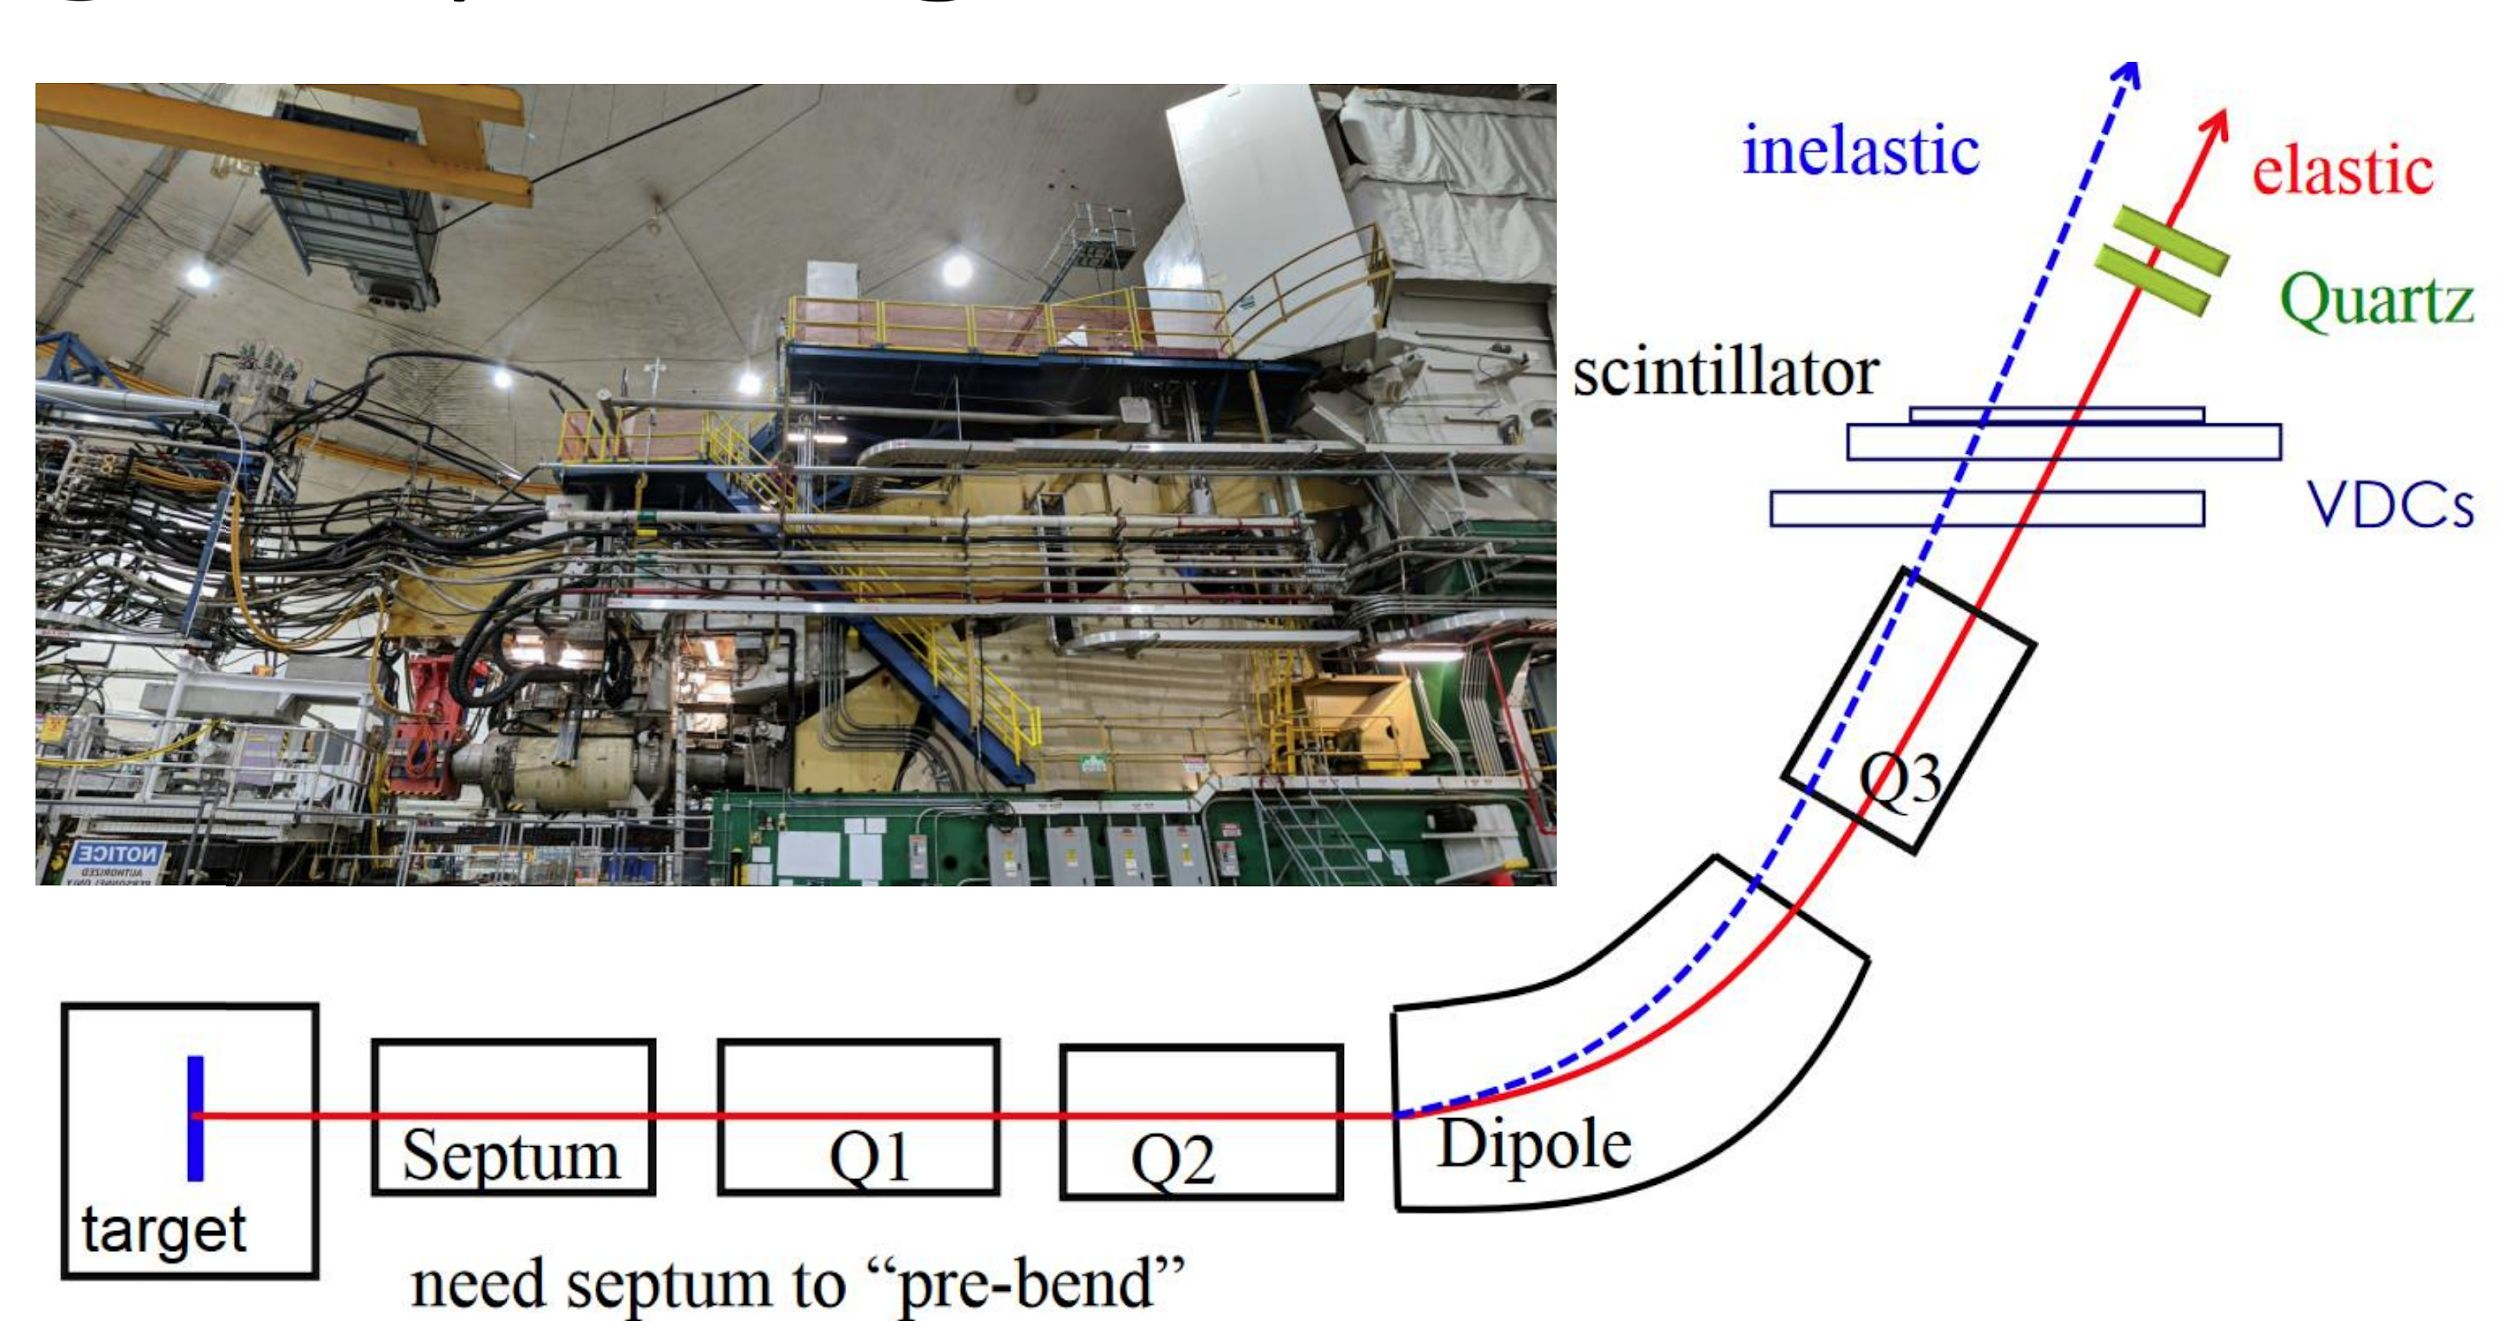
\includegraphics[width=0.8\linewidth]{HRS}
\end{figure}

%%%%%%%%%%%%%%%%%%%%%%%%%%%%%%%%%%%%%%%%%%%%%%%%
\subsection{Detector}
Quartz detector with phototubes (PMT) to detect Cherenkov radiation
the counting uncertainty will be:
\begin{equation}
    \sigma = \sigma_{stat}\sqrt{1 + \sigma^2_{res}}
\end{equation}

%%%%%%%%%%%%%%%%%%%%%%%%%%%%%%%%%%%%%%%%%%%%%%%%
\subsection{Data AcQuisition (DAQ)}
We use to pseudo random number generator to decide the helicity pattern, which
will trigger the data taking of both detectors and monitors. DAQ will read data
from PCs, BPMs, BCMs and detectors, which will then be digitalized by a 18 digits
ADC. In one helicity window, they will sample ??? times, which will be grouped
into 4 blocks. The sum of the 4 blocks was what we got.

The integrated response of each detector and beam monitor was collected and sampled 
by a custom 18-bit ADC for each helicity window.

